\documentclass[11pt]{article}

\usepackage[utf8]{inputenc}
\usepackage{relsize}
\usepackage{authblk}
\usepackage{array}

\usepackage[table]{xcolor}
\usepackage{amssymb}
\usepackage{amsmath}
\usepackage{mathbbol}
\usepackage{bbm}
\usepackage{amsthm}
\usepackage{pdfpages}
\usepackage{graphicx,color,psfrag}
\usepackage{epstopdf}
\usepackage{pdflscape}
\usepackage{tabularx}
\usepackage{longtable}
% \usepackage{breakurl}
\usepackage{enumitem}
\usepackage[normalem]{ulem}
\usepackage{blindtext}
\usepackage{fancyhdr}

% \setlength{\headheight}{13.6pt}

\usepackage{newpxtext}

% caption fonts
\usepackage[font={large,bf}]{caption} 

\usepackage{setspace}
\usepackage{longtable}
\usepackage{threeparttable}  
\usepackage{tabulary}
\usepackage{booktabs}
\usepackage{float}
\usepackage{caption}
\usepackage{subcaption}
\usepackage{rotating}
\usepackage[titletoc,title]{appendix}

\usepackage{array,multirow}

\usepackage[round]{natbib}
\bibpunct{(}{)}{;}{a}{,}{;}
\setcounter{MaxMatrixCols}{10}

% \topmargin=-1.8cm \textheight=23.8cm \oddsidemargin=-1cm
% \evensidemargin=-1cm \textwidth=18.5cm
\usepackage[margin=1in]{geometry}
\newtheorem{ass}{Assumption}
\newtheorem{definit}{Definition}
\newtheorem{prop}{Proposition}
\newtheorem{cor}{Corollary}
\newtheorem{thm}{Theorem}
\newtheorem{lem}{Lemma}
\newtheorem{conj}{Conjecture}

\graphicspath{ {./images/} }

\usepackage{color}
\definecolor{myblue}{RGB}{0, 85, 165}
\usepackage[colorlinks=true,linkcolor=myblue, allcolors=myblue]{hyperref}
\usepackage{soul}

% \pagestyle{fancy}
% \fancyhf{}
% \rhead{\textsc{Amedeus Akira Dsouza} \textsc{(}\textit{he}\textsc{/}\textit{him}\textsc{/}\textit{his}\textsc{)} \textsc{42975961}}
% \lhead{ECON 499 003}

\cfoot{\thepage}

\title{Labor Unions and Racial Inequality}
\author{By: Amedeus Akira Dsouza\thanks{Amedeus Akira Dsouza: \href{mailto:aa_dsouza@alumni.ubc.ca}{aa\_dsouza@alumni.ubc.ca}. I am extremely grateful to Professor Nicole Fortin and Professor Marit Rehavi for their continued guidance and support. I would like to thank Professor Nicole Fortin and Neil Lloyd for providing Stata codes that expedited the data cleaning process. I would also like to thank Sheldon Birkett, Felipe Grosso, Elisabeth Hatting, Wenxin Ma, Evan Mauro, Javier Cort\'{e}s Orihuela, and Sarah Kirker Wappel for helpful discussions and comments. Codes, tables, figures, and working drafts can be found \href{https://github.com/aadsouza/econ499}{here} on GitHub.} \textsc{ (}\textit{he}\textsc{/}\textit{him}\textsc{/}\textit{his}\textsc{)}}
\affil{University of British Columbia}
\affil{Supervised by: Nicole Fortin and M. Marit Rehavi}
\date{Sunday, April 11, 2021}

\begin{document}
\begin{titlepage}
\maketitle
\centering
\vspace{2cm}
Submitted to the Vancouver School of Economics in partial fulfillment of the requirements for a Bachelor of Arts, Honours in Economics.
\end{titlepage}
\thispagestyle{empty}
\doublespacing
\begin{abstract}
Lorem ipsum dolor sit amet.
% We seek to understand the effect of labor market institutions - in particular, the minimum wage and labor unions - on racial wage inequality along the wage distribution, taking into account spillover effects -  including minimum wage ripples and labor union threat effects. We expect to use an estimation strategy involving DFL decompositions, RIF regression analyses, distribution regressions, and a difference-in-differences research design leveraging variation in state-level minimum wage increases and state-industry unionization rates. Therefore, we expect to contribute towards the literature on the disproportionate impacts of \textit{prima facie} race-neutral policies.
\end{abstract}
\clearpage
\pagenumbering{arabic}
\section{Introduction}\label{sec:intro}
\textit{Prima facie} race-neutral changes to labor market institutions including increases to the minimum wage have disparate impacts on outcomes of underrepresented workers \citep[see, for example,][]{derenoncourtmontialoux2020}. Strengthening labor market institutions - by, for example, encouraging and buttressing labor unions or increasing the minimum wage - could therefore reduce racial inequality. While targeted policies that seek to address these inequalities are indeed important, they are often limited in scope and susceptible to legal challenges. The broader question I seek to contribute towards answering is what is the effect of changes to labor market institutions on racial inequality. 

Between 1983 and 2019, the Black-white wage gap at the median has stagnated for men and exacerbated for women (see \autoref{fig:med_wage_time}). Being a Black man consistently carries an associated Black wage penalty of over 15\% relative to white men. For Black women, the associated wage penalty starts at 6.7\% in the 1983-1988 period, increasing to around 10\% in the 2000-2019 period. Black people are consistently over-represented in labor unions (see \autoref{fig:ucov_hrs_time}). However, since 1983, unionization rates for Black people have declined at a much higher rate relative to white people, with the contrast more striking for Black women relative to white women. Through the period, a series of state level right to work laws that weaken labor unions have been enacted, thereby providing a mechanism by which one can price this declining unionization rate in terms of wages. A first order question then is whether the Black-white wage gap has exacerbated as a consequence of these right to work laws, if so, by how much, and where in the wage distribution are these effects the strongest. I also ask how much of this effect is driven by spillovers. Spillover effects capture the idea that in highly unionized environments, firms whose employees are not covered by a union may raise wages to minimize potential unionization threats. 

I find that laws that weaken unions appear to increase Black-white wage inequality with the effects concentrated at the bottom of the wage distribution and among women. Specifically, I find that for women, in addition to a baseline decrease in wages of over 3\%, right to work laws lead to a disproportionate 3.88\% decline in wages for Black women. These disproportionate effects are largely driven by spillovers. In addition to the baseline 2.51\% decline in wages for women not covered by a union, there is an additional 2.78\% decline in wages for Black women not covered by a union. Further, these dispropotionate spillover effects of the right to work legislation are harshest around the twentieth centile of the wage distribution, the same place where the associatied surplus union premium for Black women is the strongest.

The remainder of the thesis is organized as follows. I thoroughly review the literature in \hyperref[sec:lit]{Figure~\ref*{sec:lit}}. I briefly describe the dataset, present summary statistics, and characterize associations between union coverage and racial inequality in \hyperref[sec:data]{Figure~\ref*{sec:data}}. \hyperref[sec:did]{Figure~\ref*{sec:did}} estimates and presents the result of the effect of right to work legislation on Black-white wage inequality at the mean and along the wage distribution. \hyperref[sec:disc]{Figure~\ref*{sec:disc}} discusses these results and goes over robustness checks and caveats. \hyperref[sec:conc]{Figure~\ref*{sec:conc}} concludes.
% The broader question we seek to contribute towards answering is what is the effect of changes to labor market institutions on racial inequality. We expect to narrow this question down in multiple ways. First, we ask what are the effects of the decline of labor unions and changes to minimum wages on Black-white earnings inequality along the wage distribution taking into account spillover effects. We also ask how changes to the state-level minimum wage after 1970 affect the racial earnings gap.

% We observe that emerging literature shines a spotlight on the efficacy of \textit{prima facie} race-neutral changes to labor market institutions on the outcomes of underrepresented workers \citep[see, for example,][]{derenoncourtmontialoux2020}. We note that this is not exclusive to labor markets. These analyses are a subset of the broader literature that looks at the disproportionate impacts of \textit{prima facie} race-neutral policies \citep[see, for example,][]{ahs2011}.  Strengthening labor market institutions -  by for example, increasing the minimum wage or encouraging and buttressing labor unions - could therefore potentially contribute towards reducing racial inequality. While targeted policies that seek to address these inequalities are indeed important, they are often limited in scope and susceptible to legal challenges.


% \citet{derenoncourtmontialoux2020} shows us in \ref{fig1} the unadjusted Black-white earnings gap at the mean over time using data both from the CPS March Supplement and the decennial census. We clearly see that although the gap at the mean was reducing through the sixties and seventies, we start to have stagnation sometime around 1980 - and, if anything, we start to see a mild increase in the earnings gap at the turn of the twenty-first century. While the analysis put forth in \citet{derenoncourtmontialoux2020} zones in on the period of racial earnings convergence in the sixties and seventies, looking at the second panel of the plots in \ref{fig2} by \citet{barany2016}, we notice that periods of decrease in the real minimum wage may contribute towards the stagnation in the racial earnings gap after 1979. We note that \ref{fig1} only shows us the first moment which certainly does not characterize the whole earnings distribution. We see the non-uniformity of the distribution of the Black-white earnings gap smoothed for year fixed effects in \ref{fig3} by \citet{heywoodparent2012}. We observe the decline in private-sector unionization rates through the eighties and beyond as shown in \ref{fig4} but note the changing roles unions may have played over time and heterogeneity among unions at a given time with regards to racial inequality. We also note the consistent over-representation of Black people in private-sector unions.

% We expect to use the cleaned CPS dataset from \citet{fll2019} as a starting point or to follow closely the cleaning procedure that gets the CPS May and MORG datasets to match \citet{fll2019}. We will closely follow the implementation of RIF on DFL in \citet{heywoodparent2012} who studied the effect of performance pay on racial inequality along the earnings distribution. We expect to manipulate the RIF regression following \citet{fll2019} to account for spillover effects. We will run a difference-in-differences regression leveraging state-level variation following \citet{cdlz2019} and \citet{derenoncourtmontialoux2020}. Our analysis would follow the same period as \citet{cdlz2019} but would look specifically at racial inequality, not just racial demographic heterogeneity. 
\section{Literature Review}\label{sec:lit}
\subsection{Labor Unions and Racial Inequality Literature}
The relationship between labor unions and racial wage inequality has long piqued cross disciplinary interest across the social sciences, including sociology \citep[see, for example,][]{rosenfeldkleykamp2012, mccall2001} and economics \citep[see, for example,][]{ashenfelter1972, boundfreeman1992}, and the racial aspect of unions and their members has been studied in the political sciences as well \citep[see, for example,][]{frymergrumbach2020}. It has been a while since this question has been thoroughly explored in published economics research. Since the eighties, convergence in the median Black-white wage gap for men has stalled and for women has even widened. In this paper, I seek to revisit this relationship - I am interested in studying the effect of labor unions on the Black-white wage gap along the wage distribution taking into account spillover effects of policies that impact unions.

\citet{donohueheckman1991} explain that "the story of Black economic progress is not one of uniform secular advance, but rather of episodic change". Several policies and institutions have been evaluated for their potency and the mechanisms by which they reduce racial inequality, including the minimum wage \citep[see, for example,][]{derenoncourtmontialoux2020}, the Civil Rights Act of 1964 \citep[see, for example,][]{heckmanpayner1989, fgbh1973}, government transfer programs \citep[see, for example,][]{butlerheckman1977}. Factors that have been implicated as determinants of the Black-white gap include a focus on characteristics prior to labor market entry such as a skills gap \citep[see, for example,][]{nealjohnson1996}, parenting differences \citep[see, for example,][]{abhs2015}, and a college education \citep[see, for example,][]{abh2010}. The literature also alludes to under-representations of Black-white earnings inequality due to the growing absence of Black men in the workforce, in particular, due to incarceration \citep[see, for example][]{bayercharles2018, nealrick2014}. \citet{muellersmith2015} documents the persistent negative effects of incarceration on employment outcomes and on earnings. \citet{miller2017} show that federal affirmative action programs had a significant effect on the percent of Black employees which persisted after the program was rendered moot.

A growing literature has sought to evaluate changes to labor market institutions and their effect on wage inequality \citep[see, for example,][]{fll2021, fhkn2021, clr2020, ams2016, ffl2009, dfl1996}. \citet{clr2020} document the contrasting decline of unionization in the private-sector and rise of unionization in the public sector. They explain that it thus follows that public sector unions have a larger effect on wage inequality. Using Gallup polling data going as far back as 1936, \citet{fhkn2021} show that unions indeed contributed to the fall in income inequality through the forties. Looking beyond class-based perspectives, studies have also sought to approach inequality through demographic-specific analyses \citep[see, for example,][]{biasisarsons2020, blaukahn1996}. \citet{biasisarsons2020} look at the effect of flexible pay on the gender wage gap for teachers. In particular, they leverage the Wisconsin Budget Repair Bill (Act 10) that, among other things, placed severe limitations on the power of collective bargaining in public sector unions. \citet{biasisarsons2020} explain that as collective bargaining agreements expired, some school districts adopted a flexible pay model - including individual negotiations with teachers - which contributed to an increase in the gender wage gap. It is also possible that the presence of unions in the industry presents a barrier of hesitancy to firms with non-union workers seeking to adopt models such as flexible pay and performance pay.

\citet{ashenfelter1972} seeks to understand the effect of labor unions on racial discrimination in labor markets. He finds that on average racial discrimination is less prevalent in labor markets that are unionized but cautiously notes the presence of racial discrimination by labor unions themselves in the late sixties. This echoes the changing roles unions have played over time and the heterogeneity among unions in any given time as discussed by \citet{frymer2007} - from once being discriminatory and exclusionary, being indifferent about racial discrimination, to taking on leadership roles in the fight for civil rights. \citet{ashenfelter1972} also observes that the presence of labor unions had a positive effect on narrowing the Black-white wage gap over the same time period. \citet{leigh1978} is fascinated by the finding in \citet{ashenfelter1972} that craft unions - in contrast with industrial unions - had exacerbated the Black-white wage gap for men. \citet{leigh1978} also confirms said findings in \citet{ashenfelter1972} by looking at "middle-aged men". \citet{boundfreeman1992} explain that, among other factors, deunionization contributed to an increase in the Black-white wage gap among young men in the eighties. My work is distinct from \citet{ashenfelter1972}, \citet{leigh1978}, \citet{boundfreeman1992} as I will be employing econometric tools that were developed after these papers were published, in particular RIF-regression analysis which allows one to characterize the effect along the wage distribution, and will be studying the effects of right to work legislation on racial inequality - policies that do not drive their analysis. Further, the focus of discourse in the economics profession has shifted away from studying the effect of labor unions on racial inequality.

\citet{rosenfeldkleykamp2012} seek to understand the relationship between deunionization in the private-sector and racial wage inequality. Through counterfactual analysis, they find that deunionization contributes to exacerbating the Black-white wage gap - with the effect being stronger for women than for men. They explain that deunionization disproportionately affects Black workers as they are more likely to be in unions than white workers. They argue that the demand for protection against discrimination drives the over-representation of Black workers in unions. Similarly, they present that the difference between unionization for Black women relative to white women is greater than the difference for Black men relative to white men which explains the difference in the strength of the effect. Notably however, \citet{rosenfeldkleykamp2012} neither seem to account for spillover effects nor do they look at the effect of unions on racial wage inequality along the wage distribution. They compare the effects for union members to workers not in unions who would be "otherwise similar". This may be an issue in the presence of spillover effects - in particular union threat effects as discussed by \citet{fll2021}. As \citet{fll2021} explain, union threat effects capture the idea that firms may offer workers higher wages or higher benefits in order to placate interest in and threats to unionize. Looking at the overall distribution of racial inequality is indeed important as it allows one to understand how these labor market institutions change the shape of the wage distribution and where in the distribution the effects are strongest. \citet{heywoodparent2012}, for instance, notably find that the effect of performance pay through wage structure found in \citet{lmp2009} only applies to white people at the top end of the distribution.

Written effectively in response to \citet{ams2016}, \citet{fll2021} extend the analysis put forth in the seminal \citet{dfl1996} to include spillover effects when estimating the effect of the minimum wage on wage inequality and the effect of unions on the distribution of wages. \citet{ffl2009} develop the recentered influence function regression analysis and apply the method to understand the effects of labor unions on the unconditional wage dispersion accounting for both "within-group (same covariates)" and "between-group (different covariates)" effects. My work is distinct from \citet{fll2021}, \citet{ams2016}, \citet{ffl2009}, \citet{dfl1996} as I extend their analyses to explore heterogeneous effects by race. 

\citet{bayercharles2018} document a decline in racial earnings inequality for men from 1940 to 1970 followed by an increase in racial earnings inequality at both the median and the 90th percentile when those with non-positive earnings are included in the analyses. They suggest, but do not test, that, among other factors, changing minimum wages and declining unionization contributes towards an effect on "distributional convergence" - "changes in the shape of the overall earnings distribution that affect Black–white relative earnings because [Black men] and [white men] occupy different initial positions in that distribution".

% Our analysis indeed builds on the work put in by \citet{derenoncourtmontialoux2020} studying the effects of the minimum wage on racial inequality and is distinct in terms of the time period being studied, the better data available for the period being studied, the different dynamics of the racial earnings gap in the period being studied - in particular, the stagnation of the gap, and in the level of the policy changes being studied - federal vs. state-level changes to the minimum wage. We expect to further build on the topic in the coming weeks towards a more fruitful analysis in order to make a more significant contribution to the literature on labor market institutions and racial inequality.

\subsection{Right to Work Laws and Associated Literature}
The National Labor Relations Act of 1935 required that all people, including non-union members, who are covered by a collective bargaining agreement pay dues to unions. The Labor Management Relations Act of 1947 amended the National Labor Relations Act allowing states to pass legislation that does not permit unions to collect dues from people covered by a collective bargaining agreement or require that they join the union, "right to work" laws. Several states implemented right to work legislation through the mid-twentieth century, denoted "always right to work states" in \autoref{fig:rtwmap}. However, I am not able to exploit policy variation from these states as the NBER extracts of the CPS Merged Outgoing Rotation Groups do not have a variable identifying union coverage before 1983. I do not include policy variation from Idaho (1985) as I am concerned with the potential insufficiency of the pre-treatment period. Consistent with \citet{fll2018}, I do not include policy variation from Texas (1993) as Texas has had some form of right to work legislation since the late forties. I do leverage policy variation from "new right to work states", that is states that have recently enacted right to work legislation. These states include Oklahoma (2001), Indiana (2012), Michigan (2013), Wisconsin (2015), Kentucky (2017). I do not include policy variation from West Virginia's 2016 right to work law due to concerns about parallel trends. 

\citet{lewis1963} identifies two mechanisms by which labor unions affect the wages of people not covered by a union: "spillover effects", by which, as \citet{farber2005} explains, "workers who are no longer employed in the union sector move to the nonunion sector, resulting in an increase in labor supply in that sector that reduces the equilibrium wage" and "threat effects" where firms whose employees are not covered by a union adopt wage structures similar to unionized workplaces, that is raise wages, in order to mitigate any potential threats of unionization. \citet{fll2021} provide an alternative characterization of spillover effects suggesting that in imperfectly competitive labor markets, non union firms, in competition with union firms, may increase wages in order to attract workers. Through the paper, I use spillover effects and threat effects interchangeably in order to allude to the threat effects identified by \citet{lewis1963} and spillovers as defined by \citet{fll2021}. This is because I am not able to parse the mechanism by which the effects take place. 

Leveraging policy variation from Idaho (1985) and Oklahoma (2001), \citet{farber2005} studies the effect of right to work legislation on non-union wages and finds evidence that right to work laws are associated with a decrease in non-union wages. \citet{vanheuvelen2020} finds that right to work laws exacerbate economic inequality with heterogeneous effects across the wage distribution. \citet{ffl2009} identify largest union wage premiums at and just below the median of the wage distribution. \citet{callawaycollins2018} find that through the mid-twentieth century, the associated union wage premium was greater for Black people than for white people and was concentrated at the bottom end of the wage distirbution. \citet{taschereau-dumouchel2020} develops a theoretical foundation, illustrating the union threat effect where "to prevent their own unionization, nonunion firms distort their hiring decisions in a way that also compresses the range of wages", thereby providing a mechanism by which right to work laws weaken unions and impact non-union wages. Among other things, \citet{fll2018} revisit the right to work study by \citet{farber2005} leveraging later policy variation with a focus on legislation in the rust belt states, particularly, Indiana (2012), Michigan (2013), and Wisconsin (2015), and identify a negative effect on wages, driven partially by union threat effects. My work is indeed distinct from \citet{farber2005}, \citet{vanheuvelen2020}, \citet{taschereau-dumouchel2020}, and \citet{fll2018} as I am interested in the disproportionate effects of the legislation on the wages of Black people.

\section{Data Description, Summary Statistics, and Descriptive Analysis}\label{sec:data}
I use the National Bureau of Economic Research extracts of the Current Population Survey Merged Outgoing Rotation Groups for the years 1983 to 2019 \citep{nbercps}. I closely follow the data cleaning process outlined in \citet{fll2021}. The race variable used by \citet{fll2021} only identifies white people and non-white people. I have recovered a much richer race variable and am able to identify non-Hispanic white people, non-Hispanic Black people, and people of other races. I am also able to identify ethnicity and hispanicity. Through the rest of the paper, for the sake of brevity, I define white people to be non-Hispanic white people, Black people to be non-Hispanic Black people, and Hispanic people to be Hispanic people of all races unless specified otherwise. Each observation in my dataset represents an individual.

Data on labor union membership and labor union coverage is available in the CPS MORG for the years following 1983. I define a binary variable for union coverage that takes a value of one for non self employed people who are eligible for pay who are labor union members or covered by a union contract. I use the NBER's recommended hourly wage definition, that is, weekly earnings including overtime, tips, and commissions divided by usual hours per week - a notable divergence from \citet{fll2021} who do not include overtime, tips, and commissions. The weekly earnings variable also includes hourly workers which have been computed as earnings per hour multiplied by usual hours per week. I am unable to identify observations that work in multiple jobs. 

I drop all observations with allocated hourly wage, weekly earnings, or usual hours and am therefore forced to drop observations from 1994 and 1995 due to the absence of an allocation flag. I drop observations that are self employed and those without pay. I follow \citet{fll2021} in imputing top-coded wages with a stochastic Pareto distribution. I use Pareto parameters for 2010 and 2011 for all years after 2010. I deflate wages to 1979 dollars using the consumer price index for all urban consumers provided by the Federal Reserve of St. Louis \citep{cpiaucsl}. I drop all observations with real wages less than \$1 and greater than \$100. I drop observations with missing real log wages. I generate a uniform one digit industry variable across all years in my sample following the definitions outlined in \citet{fll2021} which I adapt to create using NBER's two digit industry variable. I use earnings weights through the analysis and use earnings weights weighed by usual hours per week for kernel density estimates. I keep observation of ages 16 to 64.

I present summary statistics for relevant variables in \autoref{tab:bhw_sumstats}. Experience is defined as age less education less six as is standard in the literature. Therefore after cleaning, I am left with over 1.5 million observations for white men and white women, over 150,000 observations for Black men, and around 195,000 observations for Black women. In addition, the sample includes around 210,000 observations for Hispanic men and around 165,000 observations for Hispanic women. By definition, union coverage is marginally higher than union membership - the difference of which is attributed to those covered by a union contract but not union members. As expected, mean real log wages are indeed higher for white people than Black people and education levels are indeed higher for women than men of the respective races. Black women, white women, Black men, and Hispanic women are over-represented in public sector jobs relative to white men and Hispanic men. 

In \autoref{fig:ucov_hrs_time}, I present union coverage time trends by hispanicity, race, and sex. In addition to the well documented fact that unionization rates in the United States have fallen over time, there exists a consistent over-representation of Black people across time relative to their white counterparts. Unionization rates also appear to decline at a much higher rate for Black people relative to white people, with the contrast more striking for Black women relative to white women. Over 36.28\% of Black men and 27.8\% of Black women were covered by a union in 1983 compared to 27.39\% of white men and 16.78\% of white women at the same time. As of 2019, these union coverage rates have dropped to 13.28\% for Black men and 11.67\% for Black women which still remain greater than the percent of white people that were unionized, specifically, 12.71\% for white men and 11.4\% for white women. 

\autoref{fig:pub_ucov_hrs_time} shows union coverage time trends specific to the private and public sectors. Looking beyond the disparities in unionization rates between the private and public sectors, the aforementioned consistent over-representation of Black people covered by a union appears to be largely driven by the private sector relative to the public sector. For instance, in 1983, 32.1\% of Black men in the private sector, 21.08\% of Black women, 23.45\% of white men, and 10.47\% of white women were unionized - figures which drop to 9.74\%, 7.31\%, 8.8\%, and, 5.05\% respectively in 2019. For the public sector, on the other hand, in 1983, 50.94\% of Black men, 44.73\% of Black women, 48.77\% of white men, and 44.35\% of white women were unionized. Relative to the private sector, there is more intertemporal volatility in public sector unionization rates for Black people even though long run public sector unionization rates hover around a relatively stable range. There is nevertheless, a sharper decline for Black people in the public sector relative to white people. The year 2019 saw public sector unionization rates at 31.99\% and 29.58\% for Black men and Black women, whereas unionization rates for white men and white women only dropped to at 39.06\% and 38.98\%.

I further break down observations by industry in \autoref{tab:nindtab} along with associated union coverage rates in \autoref{tab:unindtab}. Educational services are among the top three industries where white women and Black women are concentrated in with 15.45\% of white women and 11.81\% of Black women in the industry. Notably, 42.9\% of white women and 38.3\% of Black women in educational services are unionized. Black women and white women are also over-represented in health and welfare services where 26.63\% of Black women and 20.54\% of white women are and 14.8\% of Black women and 8.8\% of white women are unionized. While 6.1\% of Black women and 4.4\% of white women are in transportation and utilities, 36.1\% of Black women in the industry are unionized compared to 23.4\% of white women. 13.54\% of Black men and 9.89\% of white men are in transportation and utilities where 36.6\% of Black men and 32.2\% of white men are unionized. Manufacturing sees 20.34\% of white men and 18.04\% of Black men in the industry with 18.4\% of white men and 25.2\% of Black men unionized. Around 6\% of white men and Black men are in educational services where over 35\% of white men and Black men are unionized. 

Median real log wage time trends are plotted in \autoref{fig:med_wage_time}. Throughout the period being studied, that is, 1983 to 2019, any convergence in the Black-white wage gap that took place in previous periods has stalled for men and is even diverging for women. In 1979 dollars, the difference between log wages for white men and Black men in 1983 was 0.336 and in 2019 remained 0.334. It is important to reiterate here, particularly within the context of the discussion in \citet{bayercharles2018}, that my wage specification drops observations with zero earnings. For women, the Black-white wage gap at the median has, in fact, exacerbated over time. The difference between log wages for white women and Black women in 1983 was 0.118, increasing to 0.178 in 2019. 

\subsection{Wage Distributions and Counterfactual}
In addition to presenting the wage distributions for white people and Black people, I ask what the wage distribution for white people who are covered by a union would look like if they had the same covariates as Black people who are covered by a union - with a corresponding question for those not covered by a union. Covariates include education, a quartic in experience, education-experience interaction, marital status, part-time status, public sector, CMSA, 11 industry categories, 12 occupation categories, and state, quarter, and year fixed effects. I follow the \citet{heywoodparent2012} implementation of the DFL decomposition for its added dimension allowing for selection into unions. For the wage distributions for Black people $B = 1$ and white people $B = 0$ which are given as 
\begin{equation}
    g(w\mid B = 1) = \int f(w\mid x, B = 1) h(x \mid B = 1) dx
\end{equation}
\begin{equation}
    g(w\mid B = 0) = \int f(w\mid x, B = 0) h(x \mid B = 0) dx,
\end{equation}
\citet{heywoodparent2012} show that the counterfactual wage distribution for white people covered by a union with the same distribution of covariates $x$ as Black people covered by a union $u = 1$ is given by
\begin{equation}
g^c_{B=1, u = 1}(w\mid B = 0) = \int \Theta_2 f(w\mid x, B = 0, u = 1)h(x\mid B = 0, u = 1)dx,
\end{equation}
where $\Theta_2 = \frac{Prob(B = 1\mid x) Prob(u = 1\mid x, B = 1)}{Prob(B = 0\mid x)Prob(u = 1\mid x, B = 0)}$. 
Similarly, the counterfactual wage distribution for white people not covered by a union with the same distribution of covariates as Black people who are not covered by a union is given by
\begin{equation}
g^c_{B=1, u = 0}(w\mid B = 0) = \int \Theta_3 f(w\mid x, B = 0, u = 0)h(x\mid B = 0, u = 0)dx,
\end{equation}
where $\Theta_3 = \frac{Prob(B = 1\mid x) Prob(u = 0\mid x, B = 1)}{Prob(B = 0\mid x)Prob(u = 0\mid x, B = 0)}$. In order to estimate this reweighting parameter, I run probit regressions of race and union coverage on the covariates as defined. I show these wage distributions for Black people, white people, and the counterfactual white wage distribution in \hyperref[fig:dfl_men]{Figure~\ref*{fig:dfl_men}} and \hyperref[fig:dfl_women]{Figure~\ref*{fig:dfl_women}} for men and women respectively. Indeed the wage distributions for Black people are more heavily right skewed. Note that the wage distributions at the top end will be affected by the Pareto imputation procedure which does not take race into account. The difference in the skews of the distribution is much more striking for people not covered by a union. As well, the counterfactual wage distribution for white people covered by a union closely follows the actual wage distribution for white people covered by a union. For people not covered by a union, there persists a significant difference in the wage distributions when comparing the distributions for Black people to the counterfactual white distributions.   

\subsection{OLS and RIF-OLS Regressions}
Recall that I seek to understand the effect of labor unions on racial wage inequality along the wage distribution. I first proceed with the following baseline OLS regression specification that characterizes the association between log wages and union coverage for Black people and white people
\begin{equation}
    \ln(w_{ijqst}) = \beta_0 + \beta_1 Black_i + \beta_2 covered_i + \beta_3 (covered_i \times Black_i)+ X'_i\Gamma + \zeta_j + \psi_q + \lambda_s  + \delta_t + \epsilon_{ijqst},
\end{equation}
where the dependent variable $\ln(w_{ijqst})$ represents the real log wages of worker $i$ in industry $j$, quarter $q$, state $s$, and at time $t$, $covered_i$ is a binary variable which represents being covered by a union, $Black_i$ is a binary variable which takes a value of $1$ for Black people and a value of $0$ for white people. I include $X_i$ in the regression specification which captures the following covariates: education, a quartic in experience, education-experience interaction, marital status, part-time status, public sector, CMSA, and 12 occupation categories, in addition to $\zeta_j$, $\psi_q$, $\lambda_s$, and $\delta_t$ which are industry, quarter, state, and time fixed effects. I run this regression separately for men and women and separately for the periods 1983-1988, 1988-2000, and 2000-2019. Breaking down the period of study into three periods allows me to observe trends in the coefficients over time. The coefficient $\beta_1$ captures the Black wage penalty in the period relative to white people and $\beta_2$ captures the wage premium associated with union coverage for white people and Black people. The coefficient of interest, $\beta_3$, captures the additional wage premium associated with union coverage for Black people. 

I present the results of the OLS regression of real log wages on union coverage and race in \autoref{tab:naive}. After controlling for human capital controls, other covariates, and fixed effects, for Black men there exists an associated wage penalty of around 15\% relative to white men in all three periods. For men, the wage premium associated with being covered by a union appears to be weakening over time. For white men, being covered by a union is associated with a 20.92\% increase in wages in the 1983-1988 period, a 19.6\% increase in the 1988-2000 period, and a 18.65\% increase in the 2000-2019 period. Some of this weakening can be attributed to the aforementioned downward trend in union coverage rates. In addition to the increase in wages associated with union coverage for white men, being a Black man covered by a union is associated with a surplus 4.51\% increase in wages in the 1983-1988 period, a surplus 3.09\% increase in the 1988-2000 period, and a surplus 2.65\% increase in the 2000-2019 period. 

The Black wage penalty appears to be exacerbating over time for women even after adding in covariates and fixed effects. Being a Black woman is associated with 6.7\% lower wages than white women in the 1983-1988 period, 8.72\% lower wages in the 1989-2000 periods, and 9.79\% lower wages in the 2000-2019 period. The baseline association between union coverage and wages weakens over time for women as well. Being covered by a union is associated with a 18.89\% increase in wages in the 1983-1988 period, a 16.3\% increase in the 1988-2000 period, and a 12.75\% increase in the 2000-2019 period. Interestingly, the surplus associaton between union coverage and real log wages for Black women increases over the three periods in spite of the downward trend in union coverage rates. Being a Black woman covered by a union is associated with an additional 1.61\% increase in wages in the 1983-1989 period, an additional 3.42\% increase in the 1989-2000 period, and an additional 4.13\% increase in the 2000-2019 period. Therefore, union coverage crucially appears to mitigate the racial wage penalty. However, this is indeed a presentation of correlation, not causation. I expect endogeneity to be inherently present in the model as unions may organize more among less educated labor or Black people may select into unions in order to seek protection from compensation that is discriminatory.

I am interested in characterizing the association between real log wages and union coverage along the wage distirbution. Specifically, I seek to understand the association between union coverage and the unconditional quantiles of the wage distribution. Therefore, I use recentered influence functions, in particular, RIF-OLS analysis. Following \citet{ffl2009}, for quantile $q_\tau$, I define $RIF_i$ which is given by 
\begin{equation}\label{eq:rif}
    RIF_i = q_\tau + \frac{\tau - \mathbb{1}\{w_i \leq q_\tau\}}{f(q_\tau)},
\end{equation}
where $\mathbb{1}\{w_i \leq q_\tau\}$ indicates if the observed wage is less than the quantile in question and $f(q_\tau)$ is the density of the marginal wage distribution. \citet{ffl2009} show that this yields a consistent estimate of the association between the independent variable - in this case, union coverage - and the unconditional quantile $\tau$ of the wage distribution. I estimate this specification for all $\tau \in [10,90]\subseteq \mathbb{10N}$. I refrain from testing the association at higher quantiles as they may be affected by the Pareto imputation procedure which does not take race into account. 

The RIF-OLS results corresponding to the OLS regression estimates found in \autoref{tab:naive} are presented in \autoref{fig:rifols-men} for men and \autoref{fig:rifols-wom} for women. The associated Black wage penalty for men appears to peak at the twentieth percentile of the overall male wage distribution. I expect that the reduction in the Black wage penalty for men at the tenth centile over time can largely be attributed to increases in the minimum wage. However, the stagnant associated Black wage penalty for men at the mean as discussed in \autoref{tab:naive} and at the median as discussed in \autoref{fig:med_wage_time} obscures an apparent increasing Black wage penalty in the upper echelons of the overall wage distribution, thereby offsetting the reduction at the lower percentiles. \citet{fll2021} and \citet{ffl2009} find that unions have their strongest impact at and just below the median. I find that the shape of the baseline association with union coverage for men largely follows the same pattern, that the association is largest at and just below the median. The peak baseline association for men appears to move towards the median over the three periods indicating an increase in wage inequality in non-union positions over time. Interestingly, I find that for Black men relative to white men, the surplus association of union coverage is largest at the bottom end of the overall wage distribution. The surplus association for men appears to decline as one moves along the overall wage distribution and is even negative beyond the median of the overall wage distribution. A part of the story here indeed appears to be that the Black wage distribution is more heavily skewed to the right as shown in \autoref{fig:dfl_men}. The other, more fascinating part of the story appears to be that union coverage appears to have its largest surplus association for Black men in parts of the wage distribution where the associated Black wage penalty is the strongest. I expect that the decline in the surplus association for Black men over the three periods can be attributed to the sharper deunionization rates for Black men relative to white men as presented in \autoref{fig:ucov_hrs_time} and in part to increases in the minimum wage.

For women, as seen in \autoref{fig:rifols-wom}, I find the associated Black wage penalty to peak at the twentieth centile of the overall female wage distribution in the 1983-1988 period. As the periods progress, in addition to the finding that the associated Black wage penalty at the mean increases for women, it appears to be that the peak Black wage penalty moves to the median of the overall female wage distribution. The peak baseline association for women is at the seventieth percentile of the overall wage distribution, and shifts to the median through the periods. The surplus association of union coverage for Black women relative to white women appears to mirror, and therefore offsets, the Black wage penalty for women. In the 1983-1988 period, when Black-white wage inequality among women is at its peak around the twentieth centile, the surplus associated benefit from union coverage appears to be at the twentieth centile of the overall female wage distribution as well. Similarly, in the 2000-2019 period, it appears that the surplus association of wages and union coverage takes on a much smoother hump-like shape between the tenth and sixtieth quantiles, in the same period when the shape of the Black wage penalty over the distribution for women appears to be smoother. 

I run the same RIF-OLS regressions separately for white men, Black men, white women, and Black women for the three periods, with results depicted in \autoref{fig:rifols-bw-men} for white men and Black men and \autoref{fig:rifols-bw-wom} for white women and Black women. For white men, the peak association between real log wages and union coverage is indeed at and just below the median of the overall white male wage distribution, with the peak association moving closer to the median as one moves to more recent periods. For Black men, the peak association is at the seventieth quantile of the Black male wage distribution. For white women, the peak association, is at the seventieth percentile of the white female wage distribution in the 1983-1988 period, moving towards the median in later periods. For Black women, the peak association fluctuates between the sixtieth and seventieth centiles of the Black female wage distribution. This analysis underscores two things. First, the surplus associations found in \autoref{fig:rifols-men} and \autoref{fig:rifols-wom} is partly driven by the inherent differences in the wage distributions for Black people and white people as documented in \autoref{fig:dfl_men} and \autoref{fig:dfl_women}. Second, and more interestingly, in analyzing Black people and white people separately, one crucially loses information about the Black-white wage gap, that is, the Black wage penalty relative to white people and the association between wages and union coverage that appears to offset the Black wage penalty as described earlier. 

In light of the exposition by \citet{fll2021} on the importance of unionization spillover effects in getting a fuller understanding of the effect of unionization on wages - that non-union firms in state-industries with a high unionization rate may, for example, emulate the wage structures of union firms to mitigate potential unionization threats, I sought to understand the differential effects of unionization by race, capturing these spillovers. In order to do so, I follow \citet{fll2021} in using union coverage rate at a state-industry-year level as an instrument for the unionization rate. I use all 50 states, the 11 industry categories outlined in \autoref{tab:nindtab}, and the years 1983 to 2019 as part of my definition of unionization rate. Notice that no individual person here can significantly affect the unionization rate in a state-industry by merely selecting into or dropping out. This, therefore, assuages some of my earlier endogeneity concerns. I first present results from an OLS regression specification of log wages on this unionization rate, running the model separately for white men, Black men, and Hispanic men of all races who are not covered by a union, with corresponding estimates for women who are not covered by a union. Thus, the regression I run is given by
\begin{equation}
   \ln(w_{ijqst}) = \beta_0 + \beta_1 coveragerate_{jst} + X_i'\Gamma + \zeta_j + \psi_q + \lambda_s + \delta_t + \epsilon_{ijqst}, 
\end{equation}
where the dependent variable, the covariates, and the fixed effects remain as defined before. The coefficient of interest $\beta_1$, in particular its transformed form $100(e^{\beta_1} - 1)$, captures the effect of a one percent increase in unionization rate in a state-industry-year on real log wages. 

\autoref{tab:nlincovrate} shows the estimates of these union "threat" effects. The effect of the unionization rate on white men not covered by a union remains significant but trends downwards over time. A one percent increase in the unionization rate leads to a 13.77\% increase in the wages of white men in the 1983-1988 period, a 11.4\% increase in the 1988-2000 period, and a 7.06\% increase in the 2000-2019 period. For Black men not covered by a union, the estimates are imprecise, likely due to sampling variation. Alas, a one percent increase in the unionization rate leads to an increase in wages of up to 11.52\% for Black men as seen in the 2000-2019 period. The estimates for white women not covered by a union and Black women not covered by a union appear to be closer to zero. Interestingly, union threat effects as measured by the spillover effects of unionization rate appear to be strongest for Hispanic people not covered by a union. For Hispanic men, a one percent increase in the unionization rate leads to an increase in log wages ranging from 29.05\% in the 2000-2019 period to 37.03\% in the 1988-2000 period and for Hispanic women it leads to an increase ranging from 13.88\% in the 1983-1988 period to 38.82\% in the 1988-2000 period.

% We shall use the Current Population Survey (CPS) Merged Outgoing Rotation Group as our primary dataset which is available from 1979 to 2019. In order to extend our analysis on labor unions, we shall extend our data using the CPS May back to 1973. We would like to consider supplementing our analysis with values imputed from the CPS Annual Social and Economic Supplement (ASEC). We expect our data to be the transpose of the following outline
% \begin{itemize}
%     \item $n$ is the number of observations we have in our sample after cleaning the data.
%     \item survey weight allows us to make inferences about the population using survey data.
%     \item survey year records the year the survey was conducted.
% \end{itemize}
% We expect our dependent variables (Y variables) to be the following:
% \begin{itemize}
%     \item Earnings: Hourly wages (\$, CPS) consistent with \citet{fll2019}.
%     \item Employment status (Dummy, CPS).
%     \item Benefits - such as health insurance coverage (TBD, CPS).
% \end{itemize}
% We expect our independent variables (X variables) to be the following:
% \begin{itemize}
%     \item State minimum wage which we shall define as the maximum of the state minimum wage and the federal minimum wage unless state laws for specific states mandate otherwise. Several datasets for the same have been complied in the literature including Federal Reserve Economic Data from the Federal Reserve Bank of St. Louis found \hyperlink{https://fred.stlouisfed.org/tags/series?t=minimum+wage}{here}. We note that the Wages and Hour Division of the United States Department of Labor also maintains a database of changes to non-farm state-level minimum wages found \hyperlink{https://www.dol.gov/agencies/whd/state/minimum-wage/history}{here}. There also exists a dataset \hyperlink{https://equitablegrowth.org/working-papers/historical-state-and-sub-state-minimum-wage-data/}{here} that contributes towards the analysis put forth in \citet{derenoncourtmontialoux2020} We shall impute these values using the state and year variables found in the CPS.
%     \item Union coverage (Dummy, CPS) consistent with \citet{fll2019}.
%     \item Race (Dummy, CPS).
%     \item Ethnicity (Dummy, CPS).
%     \item Sex (Dummy, CPS).
% \end{itemize}
% Our covariates shall include:
% \begin{itemize}
%     \item Age (Integer, CPS).
%     \item Marital Status (Dummy, CPS).
%     \item Children (TBD, CPS).
%     \item Education (TBD, CPS).
%     \item Experience (TBD, CPS).
%     \item MSA (TBD, CPS).
% \end{itemize}
% We note that \citet{chandra2003} identifies limitations in using CPS data - in particular, the presence of selection bias due to the exclusion of incarcerated people. Therefore, we should be cautious - and attempt to correct for this bias - as it implies that the CPS potentially understates racial inequality. 

% We also intend on exploring in the coming weeks supplementing our analysis using the data from the decennial census and the American Community Survey (ACS) following \citet{bayercharles2018} which would allow for us to include these "non workers" in our analysis. Should this be possible, we could then incorporate the effect of the minimum wage on recidivism captured by \citet{aganmakowsky2018} using data from the National Corrections Reporting Program which we expect would increase the effect of the minimum wage on Black white earnings inequality.

\section{Difference in Differences and RIF-DID Analysis}\label{sec:did}
I next leverage exogenous policy variation created by state level right to work legislation that does not permit unions to collect dues from people covered by a collective bargaining agreement or require that they join the union. This is expected to and has been documented in the literature to weaken unions, thereby providing for a quasi-natural experiment that allows one to test spillover effects of laws that weaken unions. I look at the effect of this right to work law treatment on real log wages. I run the following regression
\begin{equation}\label{eq:did}
\ln(w_{ijqst}) = \beta_0 + \beta_1Black_i + \beta_2RTW_{st} + \beta_3(RTW_{st}\times Black_i) + X'_i\Gamma +\zeta_j + \psi_q + \lambda_s + \delta_t + \epsilon_{ijqst},  
\end{equation}
where $RTW_{st} = 1$ if state $s$ has a right to work law in time $t$, $Black_i$ indicates whether the observation is a Black person or a white person, $X_i$ includes the same set of covariates as above, and fixed effects are defined as before. I run this regression separately for men, women, people not covered by a union, and people covered a union. Consistent with \cite{taschereau-dumouchel2020}, I use a sample of years from 1989 to 2019. Policy variation comes from Oklahoma (2001), Indiana (2012), Michigan (2013), Wisconsin (2015), and Kentucky (2017). I do not include variation from Texas (1993) as Texas has had some form of a right to work law in place since 1947 and my sample has dropped 1994 and 1995 due to missing allocation flags. All states, except West Virginia, Montana, Maine, New Hampshire, and Vermont are in the sample. West Virginia and variation from its 2016 right to work legislation have been dropped from the analysis in order to preserve parallel trends. The latter states have been dropped for lack of common support. The coefficient $\beta_1$ captures the Black wage penalty, $\beta_2$ captures the baseline effect of the right to work law, and the coefficient of interest $\beta_3$ captures the disproportionate effect of the right to work law for Black people, that is, the effect of the legislation on the Black-white wage gap.

Difference in differences results of the effect of right to work laws on real log wages are summarized in \autoref{tab:wagstagdid}. Columns 1 and 4 show the estimates of the model as outlined in \autoref{eq:did}. The Black wage penalty is 13.41\% for men and 6.41\% for women relative to white men and white women respectively. Being in a right to work state after the legislation becomes effective leads to a baseline 3.7\% decrease in wages for men and 3.13\% decrease for women. Laws that weaken unions disproportionately affect Black people with the effects concentrated among women. Right to work laws appear to lead to an additional 3.88\% decline in wages for Black women and an additional 2.17\% decline in wages for Black men. The Black wage penalty among people not covered by a union is 14.7\% for men and 8.06\% for women. Right to work laws indeed have significant spillover effects, leading to a baseline 2.63\% decline in wages for men not covered by a union, and a baseline 2.51\% decline in wages for women not covered by a union. There exists disproportionate spillover effects for Black women. In addition to the baseline 2.51\% decline in wages for women not covered by a union, there is an additional 2.78\% decline in wages for Black women not covered by a union. There do not appear to exist disproportionate spillover effects for Black men not covered by a union beyond the baseline 2.63\% decline in wages. The direct effects of the right to work laws on the wages of those covered by a union appear to be borne equally between unionized Black people and unionized white people, that is, there are no disproportionate effects for unionized Black people. Right to work laws appear to decrease the wages of unionized men by 5.56\% and decrease the wages of unionized women by 5.89\%.

One concern raised in analyses of recent right to work legislation is that the policies are implemented in the aftermath of adverse shocks to the real business cycle such as the Great Recession and the ensuing recovery. Therefore, Columns 2 and 5 of \autoref{tab:wagstagdid} include state monthly unemployment rates, to which the results are robust. In Columns 3 and 6, the preferred specification, I replace the year fixed effects with state specific linear time trends and keep state monthly unemployment rates in the model. Estimates of the disproportionate effect are robust to the inclusion of state linear time trends. The baseline effect of right to work laws for men remains significant, but point estimate shrinks to 1.97\%, a value shared by the baseline spillover effect of the laws for men not covered by a union. Interestingly, the inclusion of state linear time trends exacerbates the baseline effect of the laws for women and women not covered by a union to a decline in wages that is as large as 5.56\% and 5.73\% respectively. For men and women covered by a union, the effect of the legislation, once state linear time trends are accounted for, is a 4.59\% decline in wages with tighter standard errors for the former and a 5.25\% decline in wages for the latter.

Following my above analysis of the association of real log wages and union coverage using RIF-OLS, I adopt a similar approach to further flesh out the difference in difference analysis of the effect of right to work laws on racial wage inequality. I run a similar series of RIF-DID. that is, recentered influence function difference in difference regressions where $RIF_i$ remains defined as in \autoref{eq:rif}, with controls and fixed effects as outlined in \autoref{eq:did}. I use the preferred specification which includes state level unemployment rates and replaces year fixed effects with state linear time trends. 

\autoref{fig:rifdid-sltt-A} and \autoref{fig:rifdid-sltt-B} contain the results of this RIF-DID regression for all (Black and white) people and people not covered by a union, where again, the latter is intended to capture spillover effects of the legislation. This RIF-DID analysis indeed corresponds to the DID analysis at the mean presented in Panels A and B of \autoref{tab:wagstagdid}. For men and women, with the inclusion of state linear time trends, the baseline effect of right to work laws appears to be similar along the wage distribution as the RIF-DID plot is tightly wrappead around the DID estimate. Notably, the disproportionate effect of the right to work laws for both Black men and Black women relative to white men and white women respectively are consistent with the RIF-OLS finding in \autoref{fig:rifols-men} and \autoref{fig:rifols-wom}. For quantiles of the overall female wage distribution below the seventieth centile, right to work laws appear to have exacerbated Black-white wage inequality for women. The laws have their sharpest disproportionate impacts for Black women at the twentieth centile of the overall female wage distribution, the same centile where the surplus association between real log wages and union coverage was the strongest. The shape of the effect throughout  the wage distribution appears to be a reflection of the shape found in the association. Similarly, the legislation has its disproportionate impact for Black men around the bottom of the overall male wage distirbution and has a positive impact, that is, reduces Black-white wage inequality in the upper echelons of the overall male wage distribution. This finding is consistent with the RIF-OLS regression in \autoref{fig:rifols-men} where it was seen that the surplus association with union coverage at quantiles above the median was negative. Although the negative effects at the bottom of the wage distribution appear to be almost twice in magnitude than the positive effects at the top of the wage distribution, thereby yielding a negative disproportionate effect of the laws for Black men at the mean. 

In highly unionized environments, firms whose employees are not covered by a union may adopt wage structures similar to those of unionized workplaces, that is, raise wages to minimize potential unionization threats. These wage structures may even be less discriminatory. Laws that weaken unions, such as the right to work laws, make these threats less credible. It is these very spillover effects that appear to largely drive the results seen along the overall wage distribution. \autoref{fig:rifdid-sltt-B} summarizes results of the spillover effects of the right to work laws, that is, the effect of the legislation on people not covered by a union. The baseline spillover effect of the laws for women also appears to be consistent with the finding in the RIF-OLS in \autoref{fig:rifols-wom} that the association is strongest at the median of the female wage distribution. The striking negative disproportionate spillover effects at the bottom of the overall wage distribution underscore the fact that looking solely at the first moment of the distribution may obscure a fuller perspective that quantile analysis provides. 

As was done for the RIF-OLS regressions in \autoref{fig:rifols-bw-men} for men and \autoref{fig:rifols-bw-wom} for women, the RIF-DID analysis is broken down further with regressions run separately for white men, Black men, white women, and Black women, with \autoref{fig:rifdid-sltt-bw-A} containing results for the effect along the overall wage distribution for the respective races and sexes and \autoref{fig:rifdid-sltt-bw-B} containing results for the shape of the spillover effects along their respective wage distributions. The effects of the right to work legislation appear to be tightly wrapped around the mean of the wage distributions by race and sex. The concentration of the surplus effect at the bottom of the wage distributions for Black people relative to white people as found in \autoref{fig:rifdid-sltt-A} and \autoref{fig:rifdid-sltt-B} appears to be largely driven by the over-representation of Black people at the bottom of the wage distribution as well as by introduction of the interaction between the Black wage distributions and white wage distributions through the Black wage penalty.

% We break down our estimation strategy into two parts. First, we will follow the \citet{heywoodparent2012} implementation of the decomposition method developed by \citet{dfl1996} (here forth referred to as the DFL decomposition) and recentered influence function (RIF) regressions with spillover effects as found in \citet{fll2019}. Next, we shall leverage variation in state-level minimum wage increases to understand the effect of the minimum wage on the racial earnings gap after 1979 in a design similar to \citet{cdlz2019}.
% \subsection{DFL Decomposition and RIF Regression}
% \subsubsection{Labor Unions and Racial Earnings Inequality}
% We want to understand what the earnings distribution for white people who are covered by a union would look like if they had the same covariates as Black people. Therefore if Black people and white people had the same education, experience, age, marital status, and children, were in the same states, in the same industries, all at the same time, what would the distribution for white people be? We expect to run these decompositions for the various permutations of race, ethnicity, and sex. We reiterate that the DFL and RIF regression we analyse closely follow the implementation in \citet{heywoodparent2012} and direct the reader to \citet{heywoodparent2012, fll2019, ffl2009, dfl1996} for a more thorough econometric review of the methods.

% As shown in \citet{heywoodparent2012}, suppose the wage distribution for Black people $B = 1$ and white people $B = 0$ were given as
% $$g(w\mid B = 1) = \int f(w\mid x, B = 1) h(x \mid B = 1) dx$$
% $$g(w\mid B = 0) = \int f(w\mid x, B = 0) h(x \mid B = 0) dx.$$
% Then, \citet{heywoodparent2012} show that the counterfactual wage distribution for white people if they had the same distribution of covariates as Black people is given by
% $$g^c_{B = 1}(w\mid B = 0) = \int \Theta_1 f(w\mid x, B = 0) h(x\mid B = 0) dx$$
% where $\Theta_1 =  \frac{Prob(B = 1\mid x) Prob(B = 0)}{Prob(B = 0\mid x)Prob(B = 1)}$.

% Similarly, \citet{heywoodparent2012} show that the counterfactual wage distribution for white people in union jobs with the same distribution of covariates as Black people is given by
% \begin{equation*}
% g^c_{B=1, u = 1}(w\mid B = 0) = \int \Theta_2 f(w\mid x, B = 0, u = 1)h(x\mid B = 0, u = 1)dx
% \end{equation*}
% where $\Theta_2 = \frac{Prob(B = 1\mid x) Prob(u = 1\mid x, B = 1)}{Prob(B = 0\mid x)Prob(u = 1\mid x, B = 0)}$.

% We note that this procedure is indeed similar to the Oaxaca-Blinder decomposition applied to the overall distribution, not just the mean. It allows us to find the effects that are explained by our covariates - what \citet{heywoodparent2012} call "composition effects", as well as the effects that remain unexplained.

% Following \citet{heywoodparent2012}, we next seek to understand how our covariates influence these explained and unexplained effects. Therefore, for quantile $q(\tau)$, we have $RIF_i$ given by 
% \begin{align*}
%     RIF_i &= q(\tau) + \frac{\mathbbm{1}(w_i \geq q(\tau)) - (1-\tau)}{f(q(\tau))}\\
%     &= \gamma_{1,\tau} \mathbbm{1}(w_i \geq q(\tau)) + \gamma_{2,\tau}
% \end{align*}
% where $\gamma_{1,\tau} = \frac{1}{f(q(\tau))}$ and $\gamma_{2,\tau} = q(\tau) - \gamma_{1,\tau} (1-\tau)$.
% \citet{heywoodparent2012} run these RIF regressions for $q_{B = 0}(\tau)$, $q_{B = 1}(\tau)$, $q^C_{B = 1}(\tau)$ and parse $\Delta_\tau = q_{B = 0}(\tau) - q_{B=1}(\tau)$ as $$\Delta_\tau = [q_{B = 0}(\tau) - q^C_{B = 1}(\tau)] + [q^C_{B = 1}(\tau)- q_{B=1}(\tau)] = \Delta^X_\tau + \Delta^g_\tau.$$
% We intend on following a similar procedure in our paper along with the extension in \citet{fll2019} to capture spillover effects. We are therefore able to move beyond the analysis of the first moment in \citet{rosenfeldkleykamp2012} to characterize the influence of labor unions along the earnings distribution on both the composition and the unexplained effects. We expect to implement the decomposition and RIF regression procedure to study the minimum wage after 1979 and racial inequality. For unions, as discussed in \citet{fll2019}, these spillover effects would include union threat effects. As \citet{fll2019} explain, firms may increase wages or increase access to benefits in order to placate any interest in organizing or potential unionization threat. For the minimum wage, \citet{fll2019} present that those weakly below the old minimum wage are not the only ones impacted by increases in the minimum wage as there may be "ripples" of an increase spilling over beyond the minimum. 
% \subsection{State Minimum Wage Increases and Racial Earnings Inequality}
% \citet{cdlz2019} note the presence of "138 prominent state-level minimum wage events, where states increased their minimum wage by at least \$0.25, and where at least 2\% of the workers were directly affected by the increase" over the time period they study - 1979 to 2016. Therefore we expect to run the following regression
% \begin{multline*}
%   \ln(w_{ijst}) = \sum_{\tau = -3}^{4}\alpha_\tau (Treat_{st}^\tau \times Black_i) +\theta_\tau Treat_{st}^\tau+ \beta Black_i +
%   \zeta_j + \lambda_s +  \delta_t + X'_{ijst}\Gamma + \epsilon_{ijst},
% \end{multline*}
% where $\ln(w_{ijst})$ are log earnings of worker $i$ in industry, state, and at time $jst$ respectively. Notice that $Treat_{st}^\tau$ tells us if the treatment, that is, the minimum wage increase takes place $\tau$ periods from time $t$ in state $s$. $Black_i$ tells us if individual $i$ is a Black person. Notice as well that, $\zeta_j$, $\lambda_s$, $\delta_t$ are industry, state, and time fixed effects respectively. $X_{ijst}$ captures the covariates we include in our model including the smaller state-level and all federal level minimum wage policy changes \citep[see,][]{cdlz2019}. These include controls for union status, education, experience, squared experience, age, squared age, sex, marital status, children, ethnicity, occupation, and number of hours worked - similar to \citet{derenoncourtmontialoux2020}. We see then that $\alpha_\tau$ is our coefficient of interest which captures the effect of the state-level increase in the minimum wage for Black people in the years preceding and proceeding the treatment. We expect our findings to be consistent with \citet{derenoncourtmontialoux2020} who found that an increase in the federal minimum wage in 1967 significantly contributed to the fall in racial earnings inequality.
% Consistent with \citet{cdlz2019} and \citet{derenoncourtmontialoux2020}, we expect to cluster our standard errors at the state-level.

% We also intend to run a quantile regression at the $90-10$ and $50-10$ differentials to get a better understanding about where the effects are the strongest. As does \citet{cdlz2019}, we would like to make use of the Kaitz index which is the minimum wage to median wage ratio in our analysis.

% As this is a difference-in-differences analysis, in addition to our ordinary least squares Gauss-Markov assumptions, we would need to ensure that common trends and excludability are satisfied. For the common trends assumption we would need that the racial earnings gap would not have changed without our treatment. For excludability, we need to ensure that there were no concurrent events affecting the racial earnings gap alongside increases to the state-level minimum wage. We are reassured by the fact that we are leveraging over a hundred policy interventions as we would need to find concurrent events that systematically bias our results in a particular direction. We intend on putting our estimates through a barrage of falsification tests. In particular, we can test arbitrary pre-treatment state-times to check if we find no effects on the racial earnings gap.

% We could also look at sub-samples where we expect the effect to be stronger - in particular youth employment. We also expect our results to be robust to controls being added to and taken away from the model. As does \citet{cdlz2019}, we could break down our analysis and run our regressions in order to test each of the individual policy changes. We explored the idea of testing people in the upper end of the distribution as a relevant subsample where we had believed it to be reasonable to not find any spillover effects. However, we learned about the findings in \citet{barany2016} who showed that increases in the minimum wage affect decisions about human capital accumulation which would significantly effect those at the upper end of the distribution. In order to enrich our analysis we indeed intending at exploring heterogeneity by demographic groups including age, sex, and ethnicity.

% With our analysis on unions, we are concerned about omitted variables including the composition of unions themselves. \citet{frymergrumbach2020} note that "white union members have lower racial resentment and greater support for policies that benefit [Black people]". Therefore, it is possible that effects we find may not be driven by the institution of unions, collective bargaining, and organizing itself, but from a collection of like-minded people that are cognizant about racial biases and discrimination. \citet{brown1984} documents that "censoring" workers who earn neither a wage nor a salary - that is those who have "dropped out" of the labor market - in published median earnings leads to an underestimation of the Black-white wage gap and suggests corrections to estimates.
\section{Discussion}\label{sec:disc}
[SYNTHESIZE INTERPRETATION OF RESULTS]

For robustness, I first run the difference in difference model without "always right to work" states, that is, states that have had right to work laws before the sample. Results of the exercise are presented in \autoref{tab:wagstagdid-wo-ar2w}. The baseline effect for men ranges from a decrease in wages by 2.13\% with the inclusion state linear time trends to a decrease by 3.54\% without, and for women ranging from a decrease in wages by 3.65\% without state linear time trends to a decrease by 5.73\% with. There remains a significant disproportionate effect for Black women relative to white women, a little over two-fifths of the effect found when estimated with always right to work states included in the specification. The disproportionate effect for Black men relative to white men becomes hard to distinguish from zero. As before, a significant amount of the effect appears to be driven by spillover effects with the baseline spillover effects being as strong as they were under the previous specification in \autoref{tab:wagstagdid} and the disproportionate effects being halved. I also present the corresponding RIF-DID regressions in \autoref{fig:rifdid-sltt-wo-ar2w-A} for all Black people and white people, \autoref{fig:rifdid-sltt-wo-ar2w-B} for spillover effects, and \autoref{fig:rifdid-sltt-wo-ar2w-C} for direct effects. 

In order to test for parallel trends, I plot real log wage trends in each of the treatment states and the never right to work states. After dropping observations from Montana, Maine, New Hampshire, and Vermont, I regress real log wages on the covariates and industry, quarter, state, and year fixed effects separately for white men, Black men, white women, and Black women. I then plot the resulting predicted real log wage trends for the never right to work states and the states that form the policy variation for the analysis: Oklahoma (2001) in \hyperref[fig:pta_ok]{Figure~\ref*{fig:pta_ok}}, Indiana (2012) in \hyperref[fig:pta_in]{Figure~\ref*{fig:pta_in}}, Michigan (2013) in \hyperref[fig:pta_mi]{Figure~\ref*{fig:pta_mi}}, Wisconsin (2015) in \hyperref[fig:pta_wi]{Figure~\ref*{fig:pta_wi}}, and Kentucky (2017) in \hyperref[fig:pta_ky]{Figure~\ref*{fig:pta_ky}}. This exercise shows that parallel trends largely appear to hold for women and white men. For Black men, sampling variation precluded us from coming to the same conclusion. Specifically, this may be a feature largely driven by the number of Black men observed in the CPS for certain states in certain years. The exercise had also revealed that West Virginia and the policy variation that comes from their 2016 right to work legislation needed to be dropped from the analysis in order to preserve parallel trends. Predicted real wage trends for West Virginia is rendered in \hyperref[fig:pta_wv]{Figure~\ref*{fig:pta_wv}} in the appendix.

I next follow a synthetic control approach which allows for a data-driven method to pick the control states from a pool of donor states. In the difference in difference model outlined before, each of the states had been given the same weighting. The synthetic control specification allows for one to construct a "synthetic" state by matching the treatment state with an optimal weighted average of the donor states in the period before the legislation has passed, thereby allowing one to estimate the difference between the new right to work state and its synthetic counterpart to find the treatment effect. In order to run the estimation following the synthetic control method, I collapse the dataset by state and year to generate panel data. Since 1994 and 1995 have been dropped due to missing allocation flags, in order to use a panel without gaps I drop all observations before 1996. The inclusion of Montana, Maine, New Hampshire, and Vermont created an unbalanced panel for the analyses for Black people indicating an underlying lack of common support. I therefore have dropped these states from the analysis. 

I estimate the specification separately for white men, Black men, white women, and Black women. The predictor set includes the collapsed state-year proportions of covariates, including proportion in each industry, occupation, quarter, and education-experience cells, average education level, a quartic in experience, proportion in part time positions, the public sector, married, in a CMSA, along with average real log wages from the entire pre-treatment period. I use the never right to work states as donor states. Results from policy variation generated by Oklahoma (2001) are presented in \hyperref[fig:synth_ok]{Figure~\ref*{fig:synth_ok}}, Indiana (2012) in \hyperref[fig:synth_in]{Figure~\ref*{fig:synth_in}}, Michigan (2013) in \hyperref[fig:synth_mi]{Figure~\ref*{fig:synth_mi}}, Wisconsin (2015) in \hyperref[fig:synth_wi]{Figure~\ref*{fig:synth_wi}}, and Kentucky (2017) in \hyperref[fig:synth_ky]{Figure~\ref*{fig:synth_ky}}. Associated weights assigned to donor states that comprise the synthetic states are presented in \autoref{tab:donor_weights_wm} for white men, \autoref{tab:donor_weights_bm} for Black men, \autoref{tab:donor_weights_wf} for white women, and \autoref{tab:donor_weights_bf} for Black women. Notice that I have treated the labor markets for white men, Black men, white women women, and Black women as separate and have found synthetic control states for each. 

As a further robustness check, I have also run a version of the synthetic control where donor states that have been dropped for Black people have also been dropped for white people, results of which are available upon request. \footnote{Results can be found in the replication package.} Unsurprisingly, I do not get as good a match for white people particularly because non-zero weights have been assigned to the states that have been dropped under certain permutations. Future research is needed in order to implement the synthetic control method on the Black-white interaction. 

Synthetic control methods reveal possible underlying heterogeneity in the effect of right to work laws on real log wages across the states that generate policy variation. The effects range from a negative effect on real log wages to no effect. Splitting the samples by state, by race, and by sex indeed makes it hard to parse out a clear effect from the noise created due to sampling variation. This also in many cases makes it difficult to come up with a good synthetic counterfactual. Hence, the synthetic control method is not my preferred estimate. Clearly as the figures show, the counterfactuals are relatively less noisy for white people in the pre-treatment period than they are for Black people. Thus, pooling the states together in a two-way fixed effects-esque difference in difference specification is preferred in order to ensure that enough observations are in the requisite subgroups. Further, spillover effects may be sensitive to anticipation in the months leading up to the legislation given that they are grounded in the environment in which the policy is enacted. For example, if the political climate heavily leans towards an anti-union environment, then potential union threats could be seen as less credible in that environment. Therefore, employers may not feel much pressure to raise wages or adopt wage structures similar to unionized workplaces or less discriminatory wage structures. Also, most right to work laws come into force as existing collective bargaining agreements expire. It is for these reasons that an event study is not an appropriate econometric tool to analyze the effects of the right to work legislation, particularly the spillover effects of the policy. 



Do not consider heaping at 50 cents, 25 cents, 10 cents, and 5 cents. - Impact on RIF regression analysis - see Autor's notes.
\section{Conclusion}\label{sec:conc}
Lorem ipsum dolor sit amet.
% \section{To-Do List}
% Please note that our list takes the format: Task - Approximate Duration - Anticipated Completion Date.
% \begin{itemize}
%     \item Create GitHub repository for version control - 1 day - November 30, 2020.
%     \item Complete THOROUGH review of minimum wage literature and racial inequality literature; build literature annotation table - 1 month - December 22, 2020.
%     \item Pin down major changes to independent and dependent variables and focus analysis - 2 weeks - December 18, 2020.
%     \item Adjust and enrich analysis building off \citet{derenoncourtmontialoux2020} - 1 month - December 22, 2020.
%     \item Holiday break for mental health - 1 week - December 31, 2020.
%     \item Practice running DFL and RIF regressions using assignments from ECON 561 - 1.5 weeks - December 31, 2020.
%     \item Download and clean CPS May and MORG datasets (if possible using cleaned data from \citet{fll2019} which would reduce duration to 1 week) - 3 weeks - January 10, 2021.
%     \item Load and merge supplementary datasets including minimum wage data, census data, ACS data, ASEC data as necessary - 3 weeks - January 20, 2021.
%     \item Prepare document with summary statistics - 1 week - January 25, 2021.
%     \item Pin down regression equations to be run - 2 weeks - Feb 14, 2021.
%     \item DFL and RIF analysis with necessary adjustments - 3 weeks - Feb 20, 2021.
%     \item State minimum wage regression analysis with necessary adjustments - 1 month - March 6 2021.
%     \item Robustness checks, falsification tests, subsampling, adding controls to model - 2 weeks, March 10, 2021.
%     \item Writing rough draft of thesis - 1 month - March 24, 2021.
%     \item Develop and implement palette and template for consistent plots - 1 week - April 3, 2021.
%     \item Final edits on thesis - 1.5 weeks - April 5, 2021. (4 day buffer to submission)
%     \item Thesis revision - 2 weeks - April 30, 2021.
% \end{itemize}

\singlespacing
\pagebreak
\bibliographystyle{apalike}
\nocite{*}
%citation rules 
%\citet{foo} outside 
%\citep[see, for example,][]{foo}
%no \citex*{}
%in bib: two authors fortinlemieuxXXXX; three authors dflXXXX.

{\footnotesize\bibliography{499data.bib}}

\pagebreak
\appendix
\newgeometry{top=0.75in,bottom=0.75in,left=0.5in,right=0.5in}
\fontsize{10}{12}\selectfont{
\section*{Figures}
\begin{figure}[h!]
\centering
    \caption{Union Coverage Time Trends}\label{fig:ucov_hrs_time}
    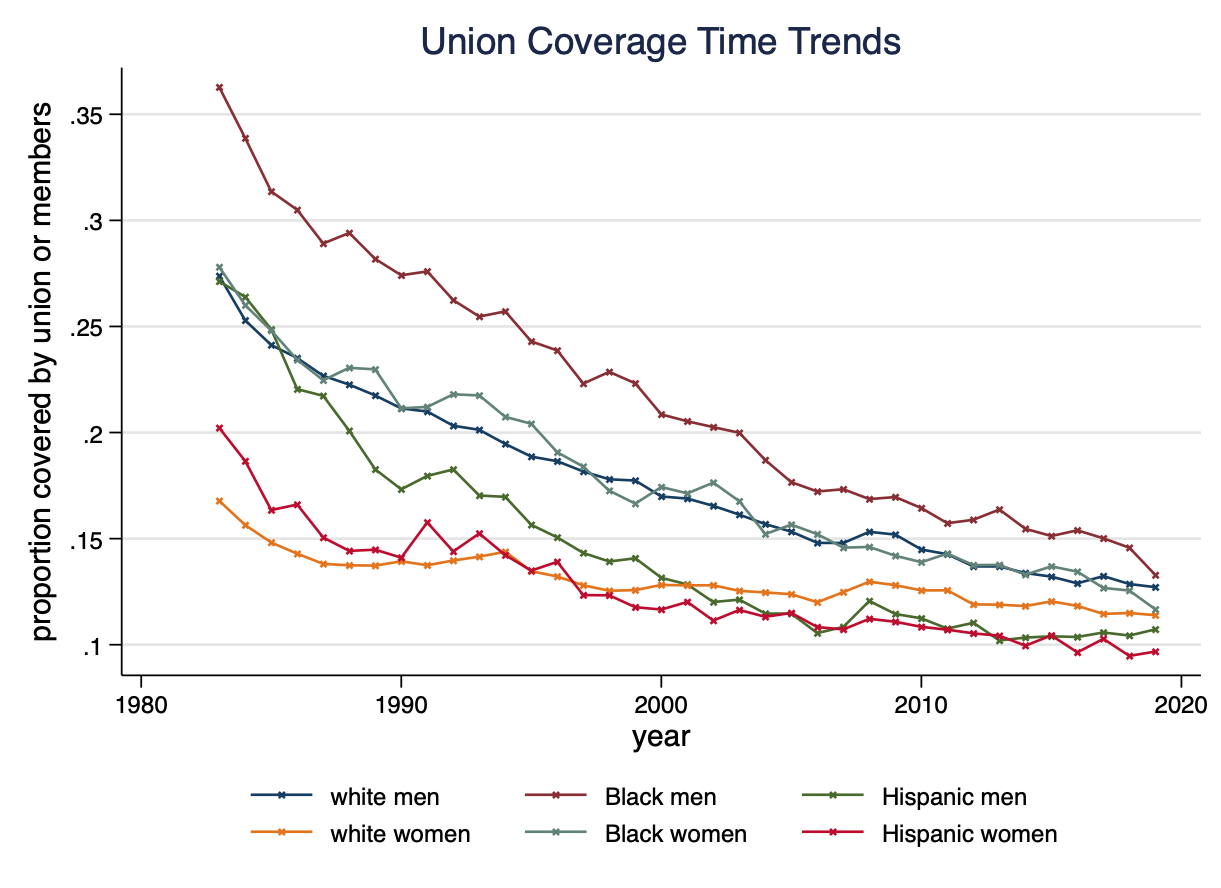
\includegraphics[width=\textwidth, height = 0.8\textheight, keepaspectratio]{figures/fin_ucov_hrs_time.png}
\end{figure}

\pagebreak
\begin{figure}[h!]
\centering
    \caption{Private and Public Sector Union Coverage Time Trends}\label{fig:pub_ucov_hrs_time}
    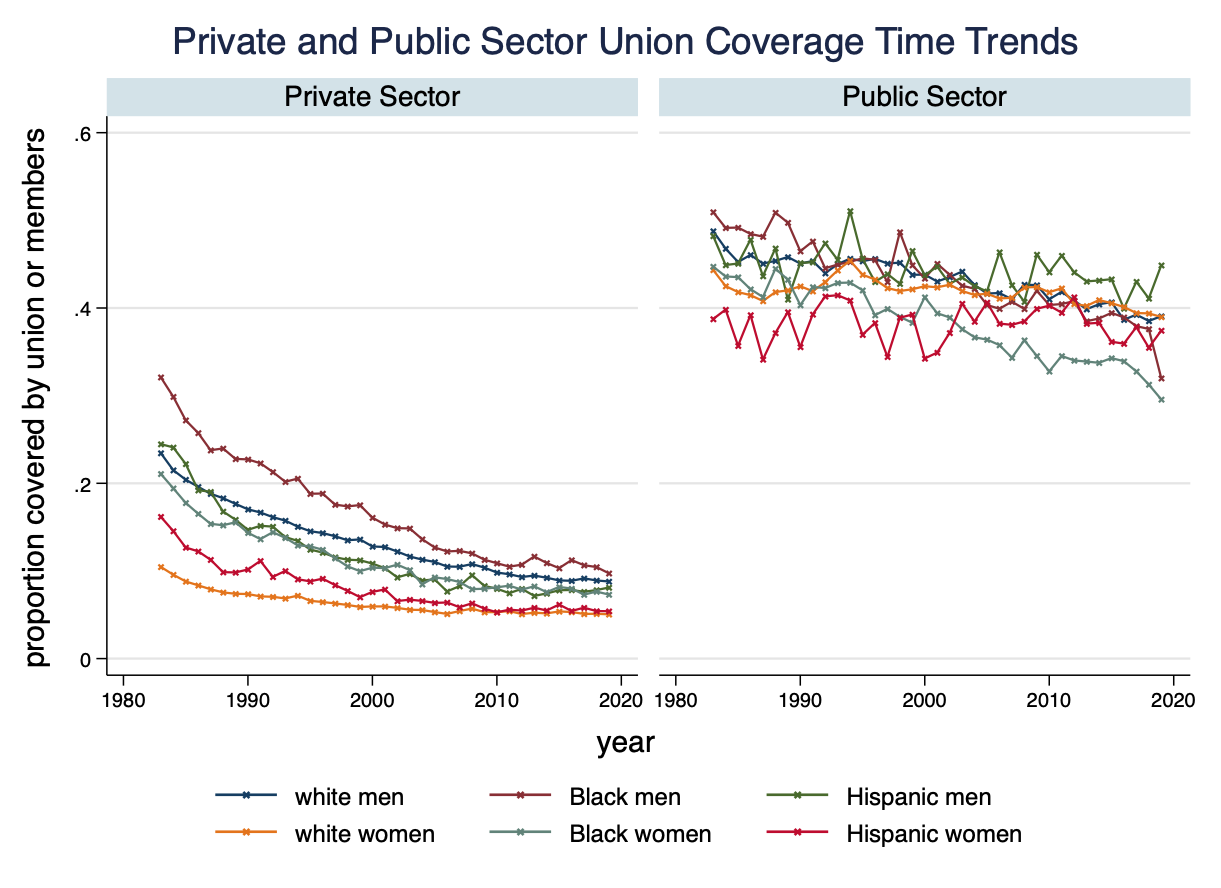
\includegraphics[width=\textwidth, height = 0.8\textheight, keepaspectratio]{figures/fin_pub_ucov_hrs_time.png}
\end{figure}

\pagebreak
\begin{figure}[h!]
\centering
    \caption{Median Real Log Wages Time Trends}\label{fig:med_wage_time}
    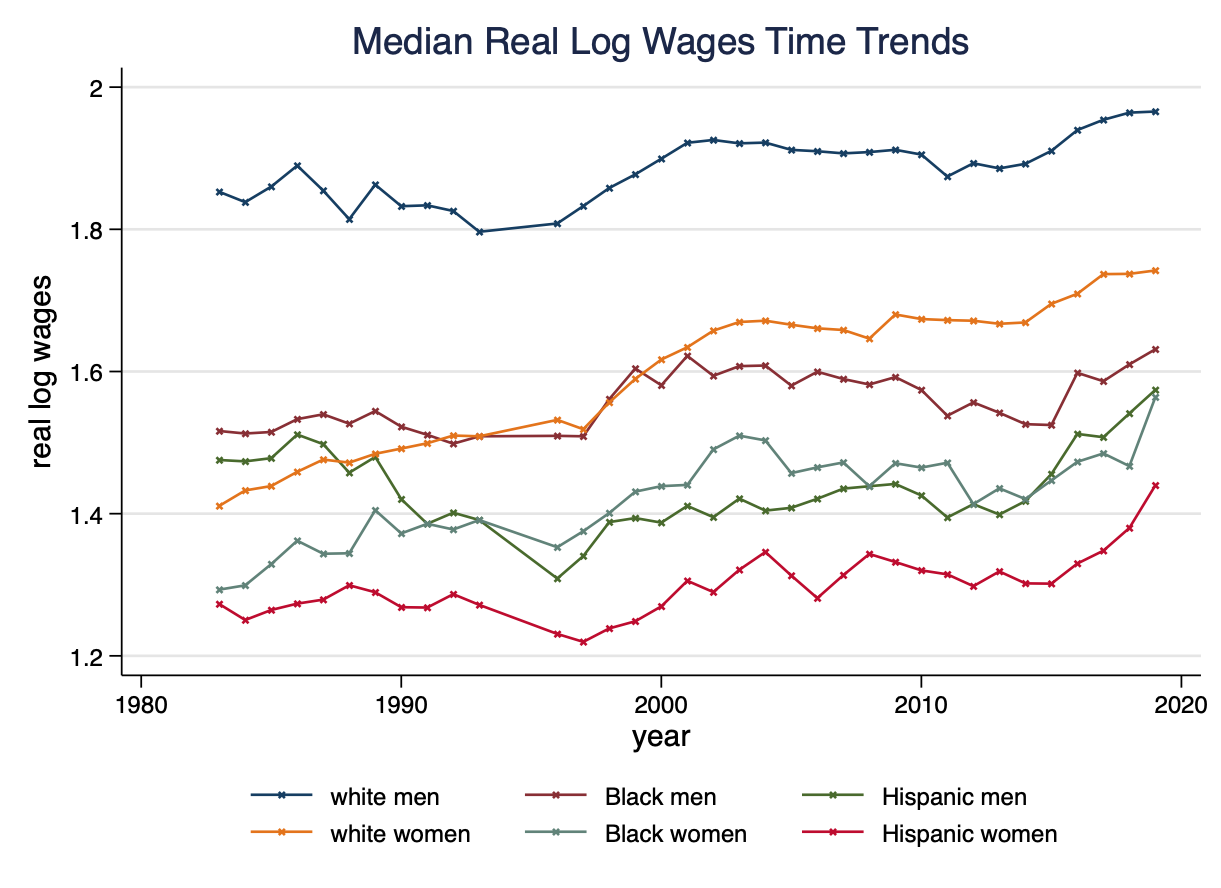
\includegraphics[width=\textwidth, height = 0.8\textheight, keepaspectratio]{figures/fin_med_wage_time.png}
\end{figure}

\pagebreak
\begin{figure}[h!]
\centering
    \caption{Right to Work States}\label{fig:rtwmap}
    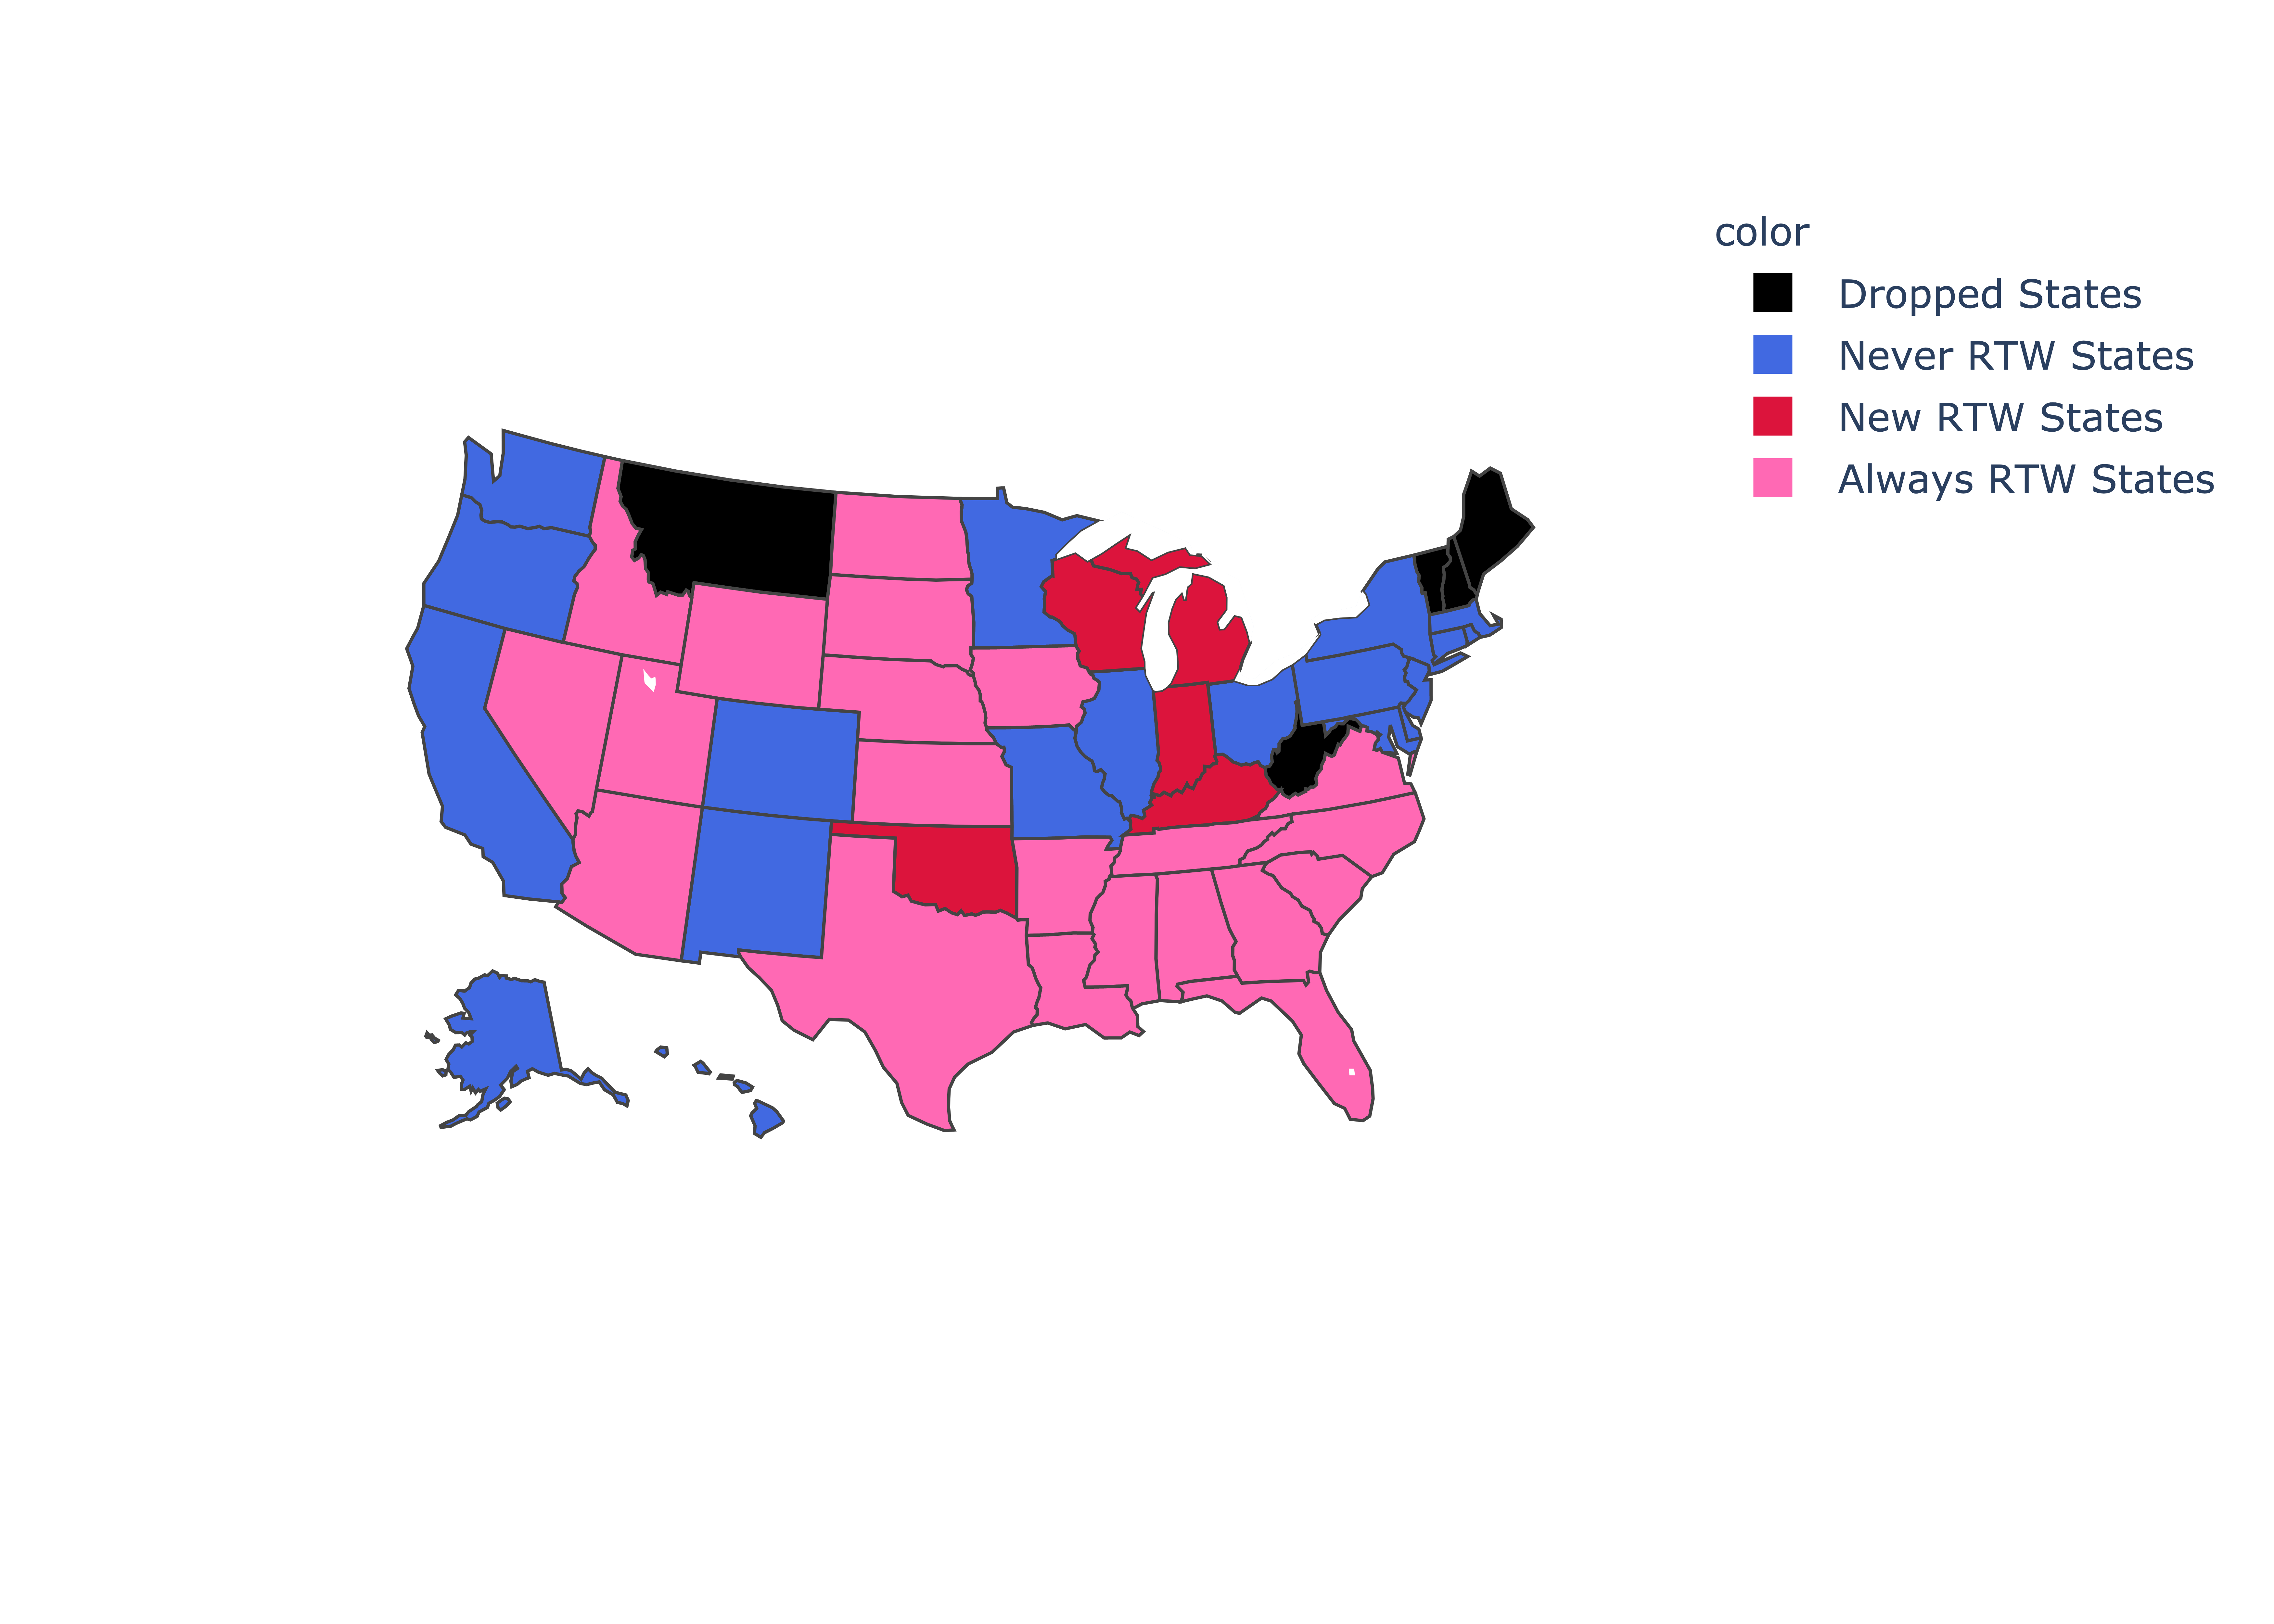
\includegraphics[width=\textwidth, height = 0.8\textheight, keepaspectratio]{figures/rtwmap.png}
\end{figure}

\pagebreak
\begin{table}[h!]
    \centering
    \captionof{figure}{Wage Distributions - Men}\label{fig:dfl_men}
    \begin{tabular}{c}
          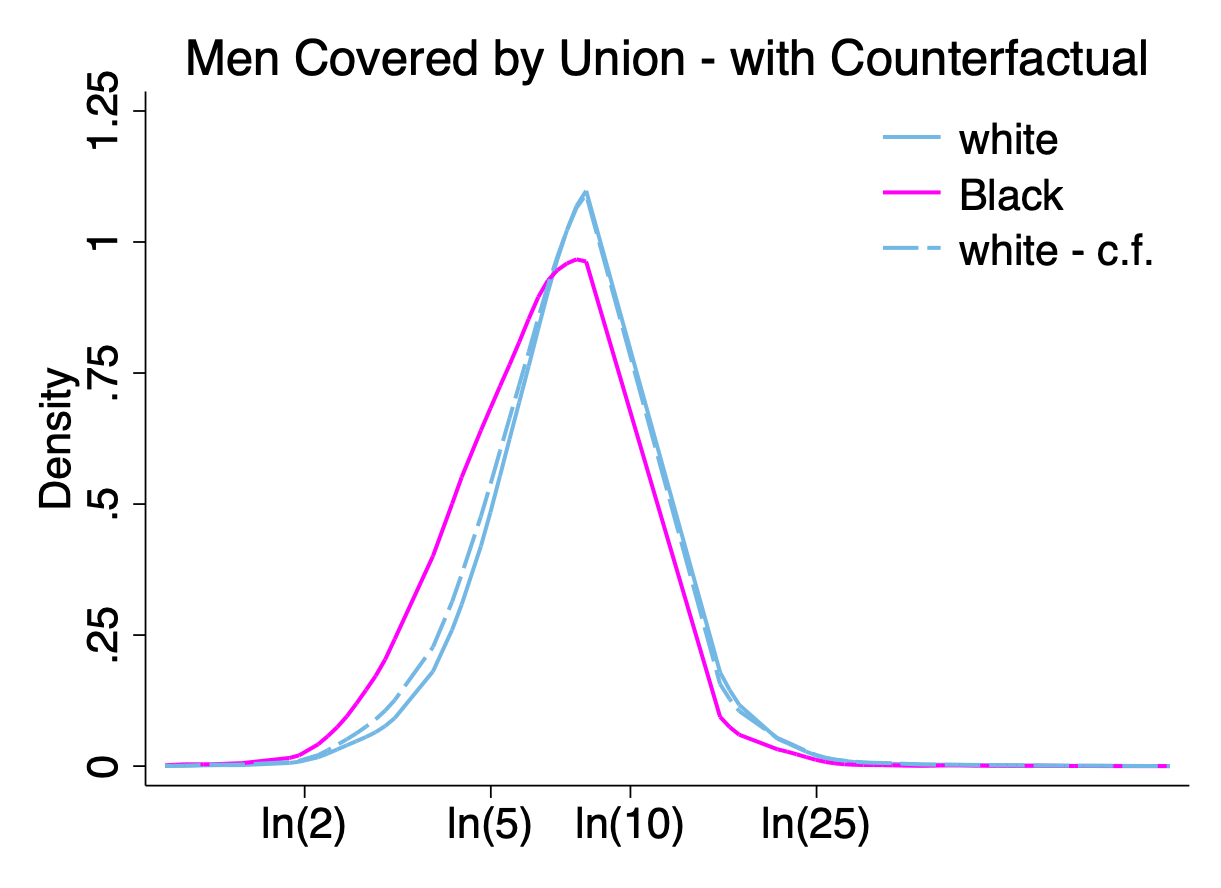
\includegraphics[width = 0.8\textwidth, keepaspectratio]{figures/kde1men/fin_cu_bhw_men.png} \\
          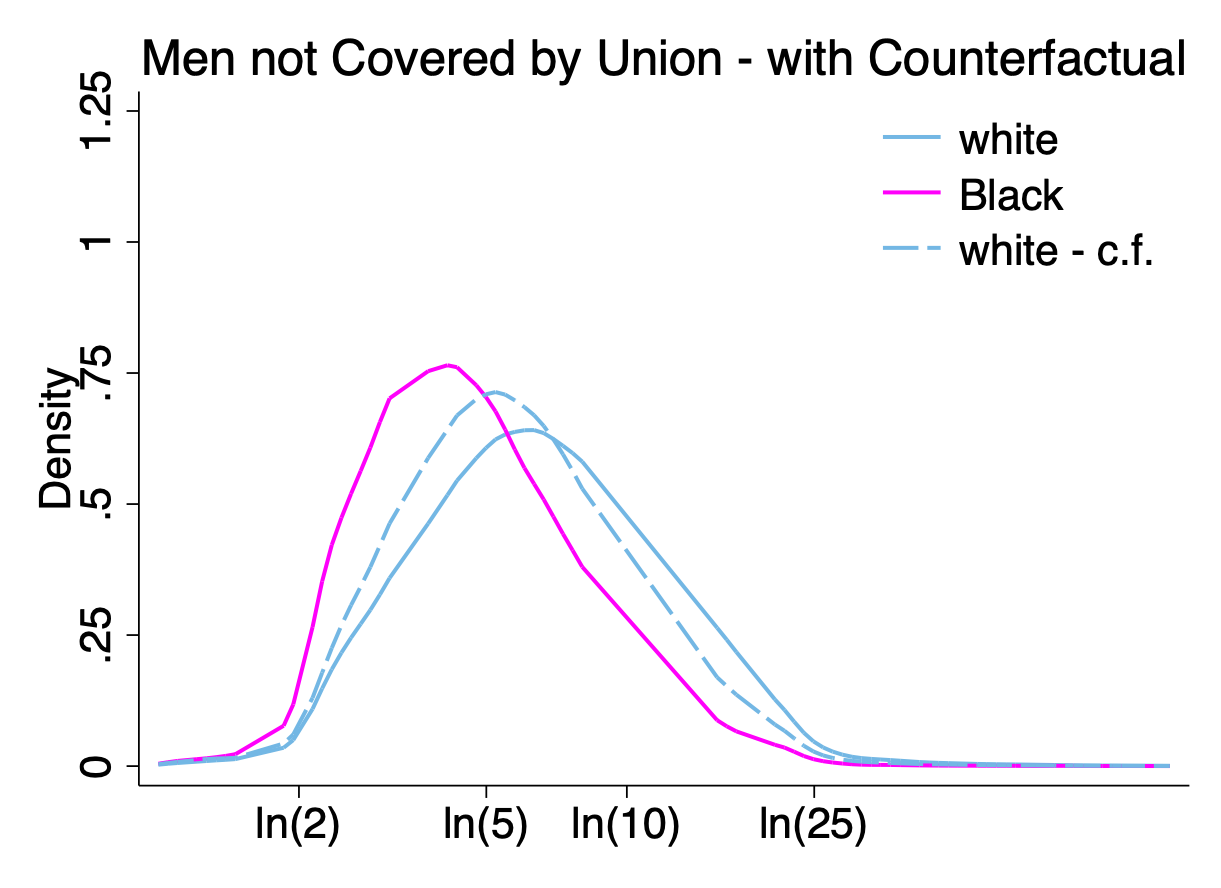
\includegraphics[width = 0.8\textwidth, keepaspectratio]{figures/kde1men/fin_cn_bhw_men.png}
    \end{tabular}
\end{table}
\footnotesize{Sample include years 1983-2019 excluding 1994 and 1995.}

\pagebreak
\begin{table}[h!]
    \centering
    \captionof{figure}{Wage Distributions - Women}\label{fig:dfl_women}
    \begin{tabular}{c}
          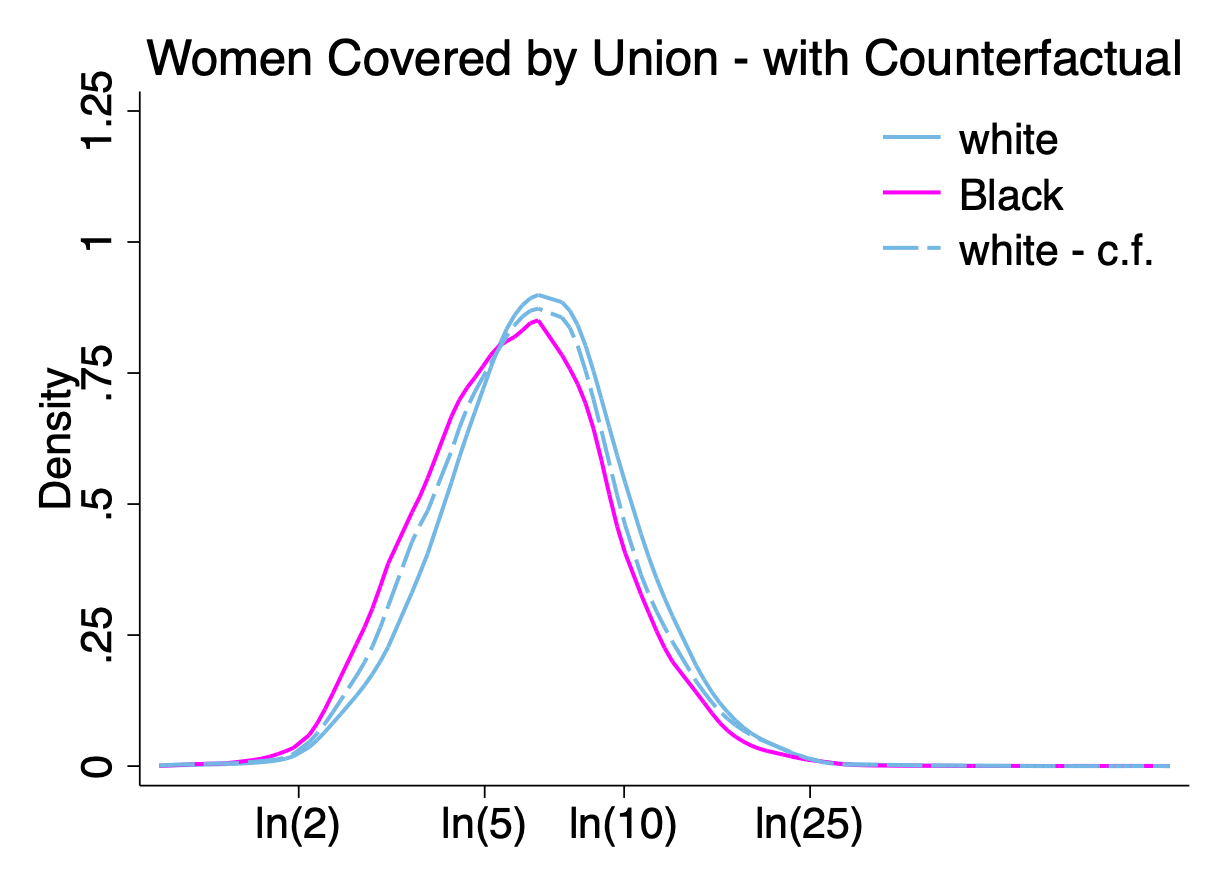
\includegraphics[width = 0.8\textwidth, keepaspectratio]{figures/kde1wom/fin_cu_bhw_wom.png} \\
          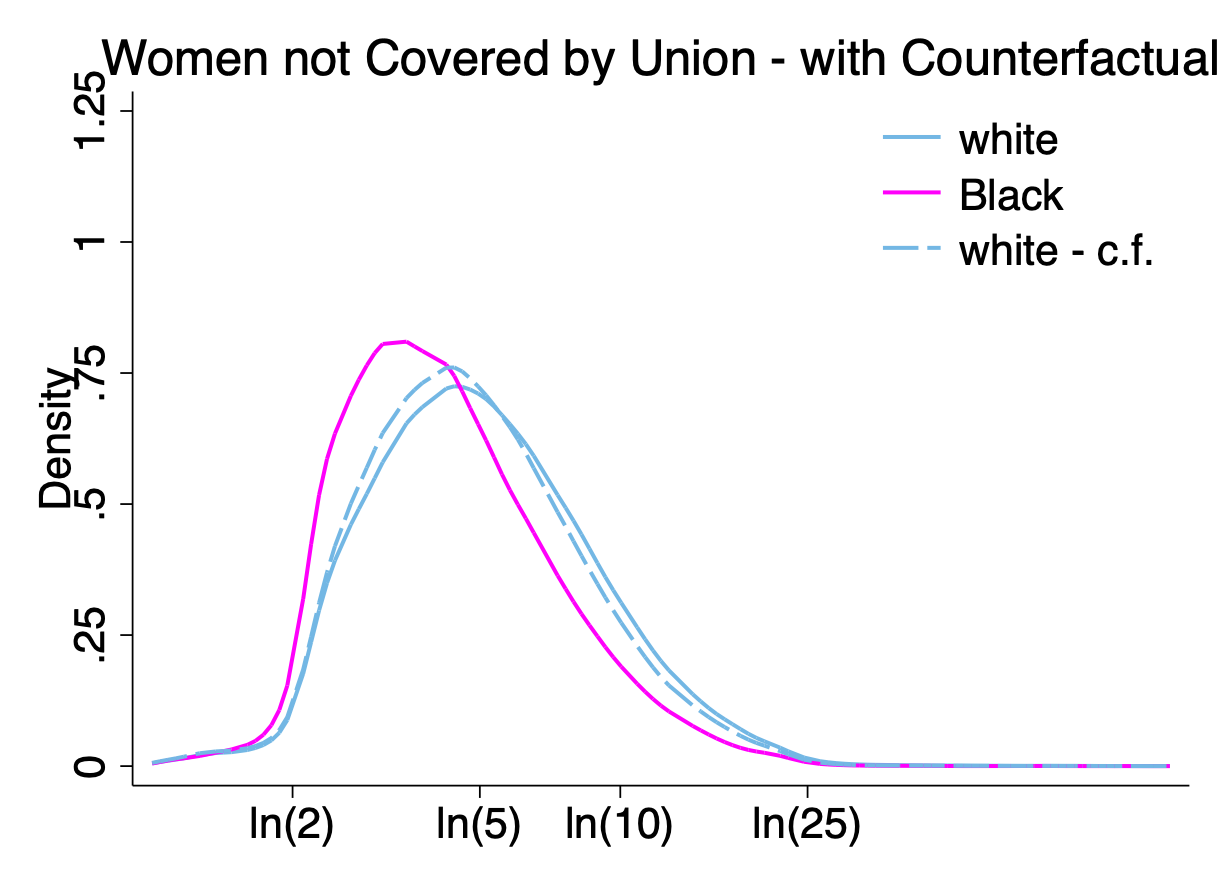
\includegraphics[width = 0.8\textwidth, keepaspectratio]{figures/kde1wom/fin_cn_bhw_wom.png}
    \end{tabular}
\end{table}
\footnotesize{Sample include years 1983-2019 excluding 1994 and 1995.}

\pagebreak
\begin{landscape}
\begin{figure}[ht!]
\centering
    \caption{RIF-OLS Regression of Real Log Wages on Union Coverage and Race - Men}\label{fig:rifols-men}
    \includegraphics[width=1.25\textwidth, height = \textheight, keepaspectratio]{figures/fin_rifols-men.png}
\end{figure}
\footnotesize{Standard errors for the OLS regression are clustered at the state-industry level. Standard errors for the RIF-OLS regression are bootstrapped with 100 replicates. Real log wages is the dependent variable throughout. Each column corresponds to a regression and associated set of RIF-OLS regressions. 95\% confidence intervals presented. All regressions include covariates and fixed effects.}
\end{landscape}

\pagebreak
\begin{landscape}
\begin{figure}[ht!]
\centering
    \caption{RIF-OLS Regression of Real Log Wages on Union Coverage and Race - Women}\label{fig:rifols-wom}
    \includegraphics[width=1.25\textwidth, height = \textheight, keepaspectratio]{figures/fin_rifols-wom}
\end{figure}
\footnotesize{Standard errors for the OLS regression are clustered at the state-industry level. Standard errors for the RIF-OLS regression are bootstrapped with 100 replicates. Real log wages is the dependent variable throughout. Each column corresponds to a regression and associated set of RIF-OLS regressions. 95\% confidence intervals presented. All regressions include covariates and fixed effects.}
\end{landscape}

\pagebreak
\begin{landscape}
\begin{figure}[ht!]
\centering
    \caption{RIF-OLS Regression of Real Log Wages on Union Coverage by Race - Men}\label{fig:rifols-bw-men}
    \includegraphics[width=1.25\textwidth, height = \textheight, keepaspectratio]{figures/fin_rifols-bw-men}
\end{figure}
\footnotesize{Standard errors for the OLS regression are clustered at the state-industry level. Standard errors for the RIF-OLS regression are bootstrapped with 100 replicates. Real log wages is the dependent variable throughout. Each sub-figure corresponds to a regression and associated set of RIF-OLS regressions. 95\% confidence intervals presented. All regressions include covariates and fixed effects. RIF-OLS for Black men in 1983-1988 period not shown due to collinearity issues.}
\end{landscape}

\pagebreak
\begin{landscape}
\begin{figure}[ht!]
\centering
    \caption{RIF-OLS Regression of Real Log Wages on Union Coverage by Race - Women}\label{fig:rifols-bw-wom}
    \includegraphics[width=1.25\textwidth, height = \textheight, keepaspectratio]{figures/fin_rifols-bw-wom}
\end{figure}
\footnotesize{Standard errors for the OLS regression are clustered at the state-industry level. Standard errors for the RIF-OLS regression are bootstrapped with 100 replicates. Real log wages is the dependent variable throughout. Each sub-figure corresponds to a regression and associated set of RIF-OLS regressions. 95\% confidence intervals presented. All regressions include covariates and fixed effects.}
\end{landscape}

\pagebreak
\begin{landscape}
\begin{figure}[ht!]
\centering
    \caption{RIF-DID Regression of Real Log Wages on Right to Work Laws Treatment in State and Time - All (Black and White) People}\label{fig:rifdid-sltt-A}
    \includegraphics[width=1.25\textwidth, height = \textheight, keepaspectratio]{figures/fin_rifdid-sltt-A.png}
\end{figure}
\footnotesize{I define $RTW_{st} = 1$ if state $s$ has a RTW law at time $t$. Sample includes years 1983-2019. Policy variation: Oklahoma (2001), Indiana (2012), Michigan (2013), Wisconsin (2015), and Kentucky (2017). All states, except West Virginia, Montana, Maine, New Hampshire, and Vermont are in the sample. Standard errors for the DID regression are clustered at the state level. Standard errors for the RIF-DID regression are bootstrapped with 100 replicates. Real log wages is the dependent variable throughout. Each column corresponds to a regression and associated set of RIF-DID regressions. 95\% confidence intervals presented. All regressions include covariates and fixed effects as outlined. State monthly unemployment rate and state linear time trends included. Year fixed effects not included.}
\end{landscape}

\pagebreak
\begin{landscape}
\begin{figure}[ht!]
\centering
    \caption{RIF-DID Regression of Real Log Wages on Right to Work Laws Treatment in State and Time - People Not Covered by Union - Spillover Effect}\label{fig:rifdid-sltt-B}
    \includegraphics[width=1.25\textwidth, height = \textheight, keepaspectratio]{figures/fin_rifdid-sltt-B.png}
\end{figure}
\footnotesize{I define $RTW_{st} = 1$ if state $s$ has a RTW law at time $t$. Sample includes years 1983-2019. Policy variation: Oklahoma (2001), Indiana (2012), Michigan (2013), Wisconsin (2015), and Kentucky (2017). All states, except West Virginia, Montana, Maine, New Hampshire, and Vermont are in the sample. Standard errors for the DID regression are clustered at the state level. Standard errors for the RIF-DID regression are bootstrapped with 100 replicates. Real log wages is the dependent variable throughout. Each column corresponds to a regression and associated set of RIF-DID regressions. 95\% confidence intervals presented. All regressions include covariates and fixed effects as outlined. State monthly unemployment rate and state linear time trends included. Year fixed effects not included.}
\end{landscape}

\pagebreak
\begin{landscape}
\begin{figure}[ht!]
\centering
    \caption{RIF-DID Regression of Real Log Wages on Right to Work Laws Treatment in State and Time - All (Black and White) People Separately by Race and Sex}\label{fig:rifdid-sltt-bw-A}
    \includegraphics[width=1.25\textwidth, height = \textheight, keepaspectratio]{figures/fin_rifdid-sltt-bw-A.png}
\end{figure}
\footnotesize{I define $RTW_{st} = 1$ if state $s$ has a RTW law at time $t$. Sample includes years 1983-2019. Policy variation: Oklahoma (2001), Indiana (2012), Michigan (2013), Wisconsin (2015), and Kentucky (2017). All states, except West Virginia, Montana, Maine, New Hampshire, and Vermont are in the sample. Standard errors for the DID regression are clustered at the state level. Standard errors for the RIF-DID regression are bootstrapped with 100 replicates. Real log wages is the dependent variable throughout. Each sub-figure corresponds to a regression and associated set of RIF-DID regressions. 95\% confidence intervals presented. All regressions include covariates and fixed effects as outlined. State monthly unemployment rate and state linear time trends included. Year fixed effects not included.}
\end{landscape}

\pagebreak
\begin{landscape}
\begin{figure}[ht!]
\centering
    \caption{RIF-DID Regression of Real Log Wages on Right to Work Laws Treatment in State and Time - People Not Covered by Union Separately by Race and Sex - Spillover Effect}\label{fig:rifdid-sltt-bw-B}
    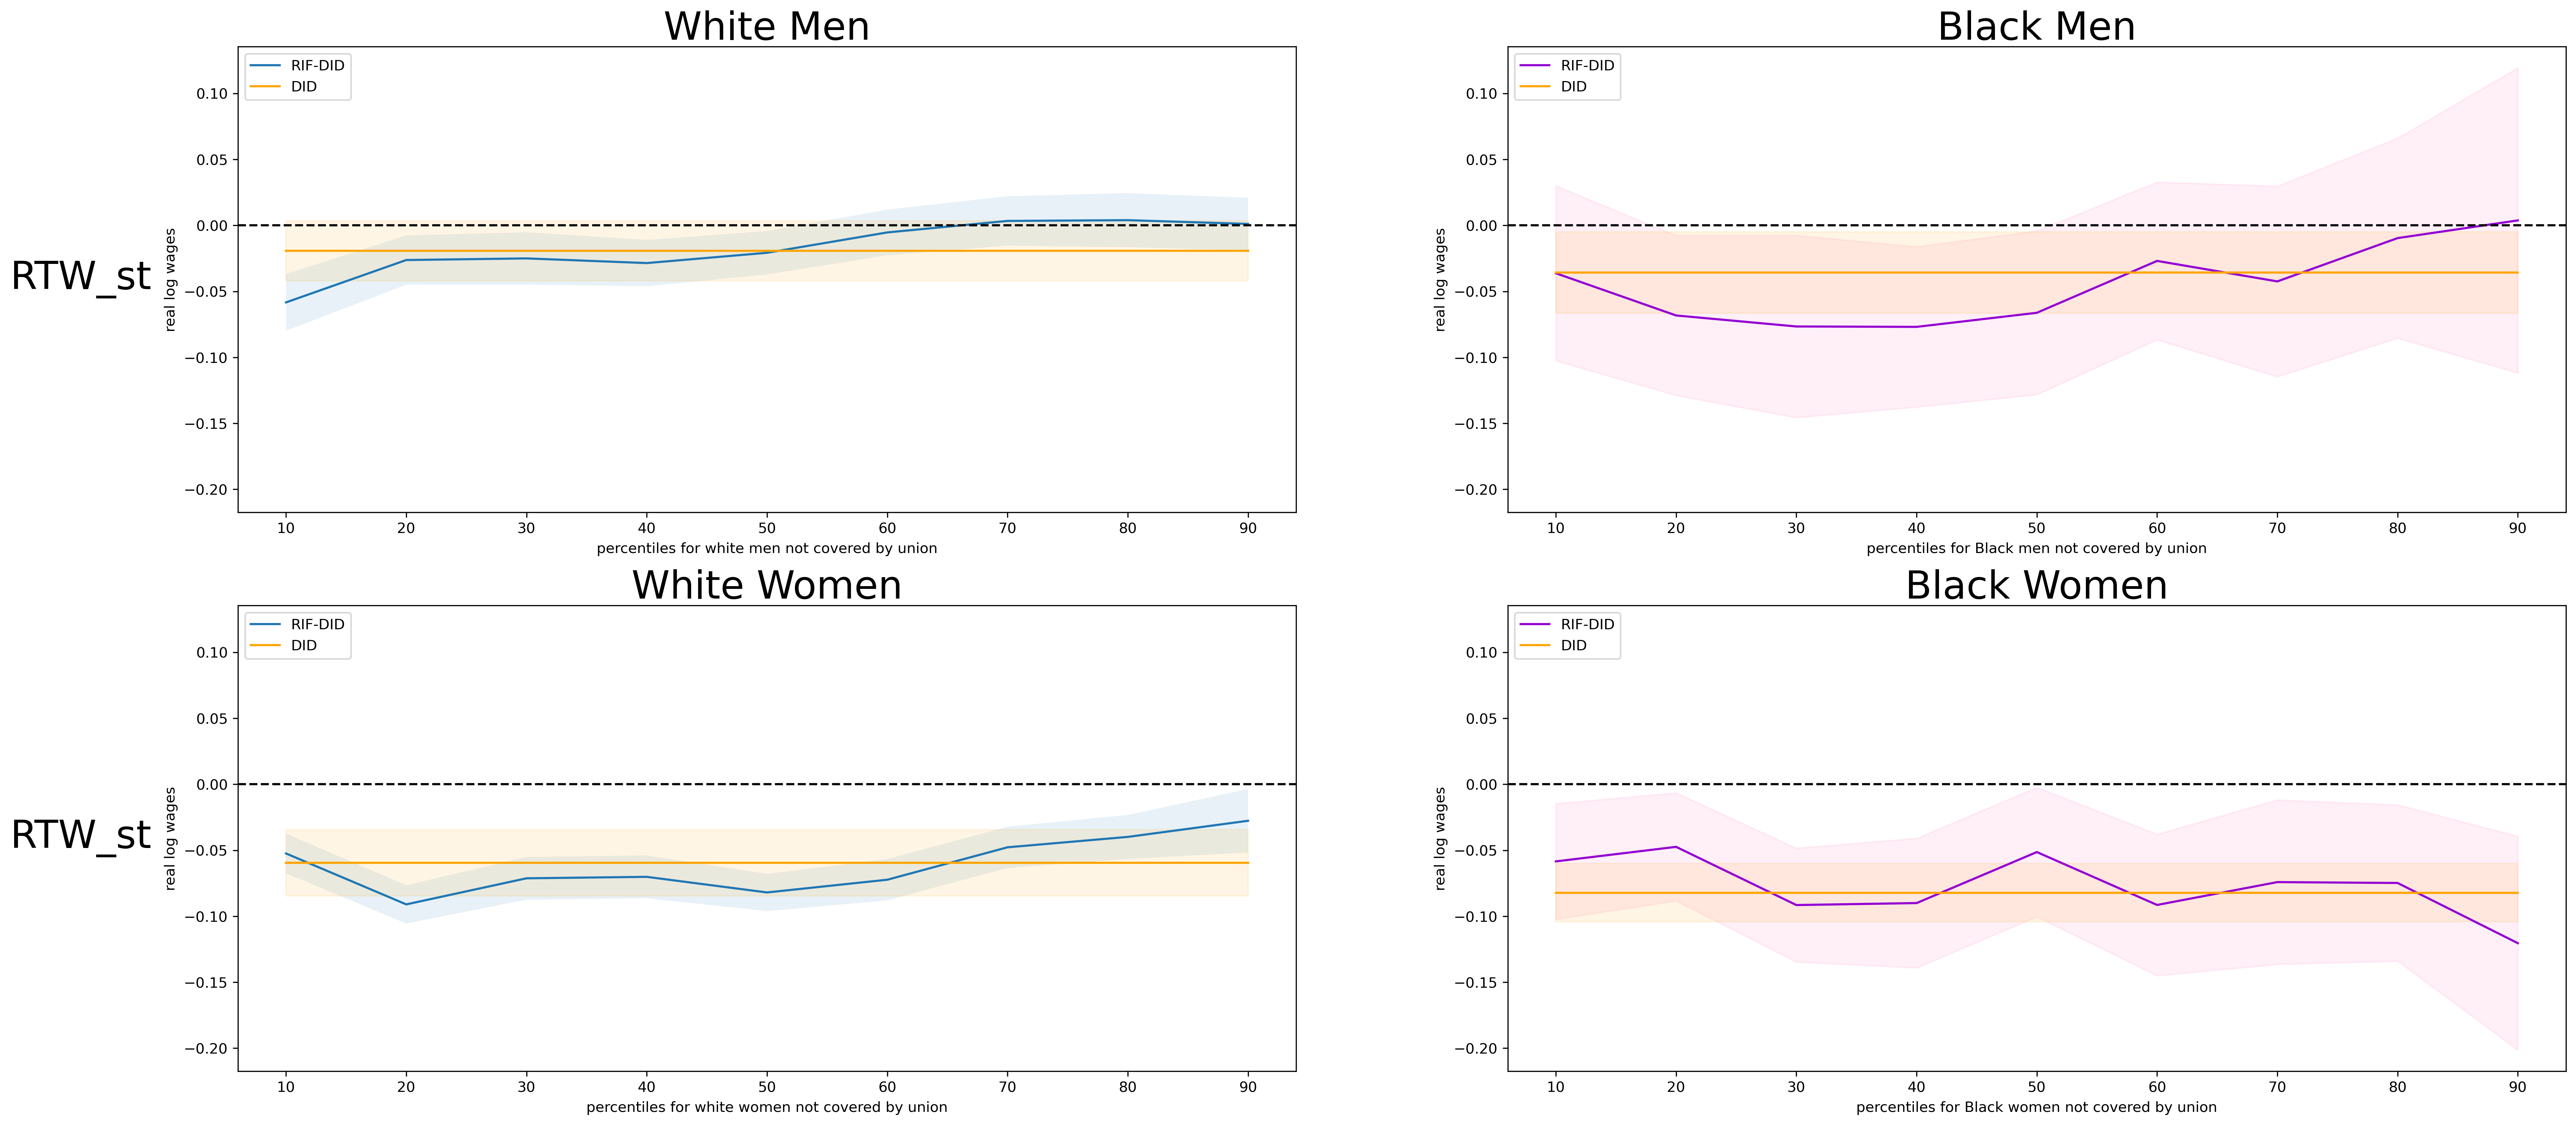
\includegraphics[width=1.25\textwidth, height = \textheight, keepaspectratio]{figures/fin_rifdid-sltt-bw-B.png}
\end{figure}
\footnotesize{I define $RTW_{st} = 1$ if state $s$ has a RTW law at time $t$. Sample includes years 1983-2019. Policy variation: Oklahoma (2001), Indiana (2012), Michigan (2013), Wisconsin (2015), and Kentucky (2017). All states, except West Virginia, Montana, Maine, New Hampshire, and Vermont are in the sample. Standard errors for the DID regression are clustered at the state level. Standard errors for the RIF-DID regression are bootstrapped with 100 replicates. Real log wages is the dependent variable throughout. Each sub-figure corresponds to a regression and associated set of RIF-DID regressions. 95\% confidence intervals presented. All regressions include covariates and fixed effects as outlined. State monthly unemployment rate and state linear time trends included. Year fixed effects not included.}
\end{landscape}

\pagebreak
\begin{landscape}
\begin{table}[h!]
    \centering
    \captionof{figure}{Predicted Real Log Wage Trends - Oklahoma (2001)}\label{fig:pta_ok}
    \begin{tabular}{c c}
          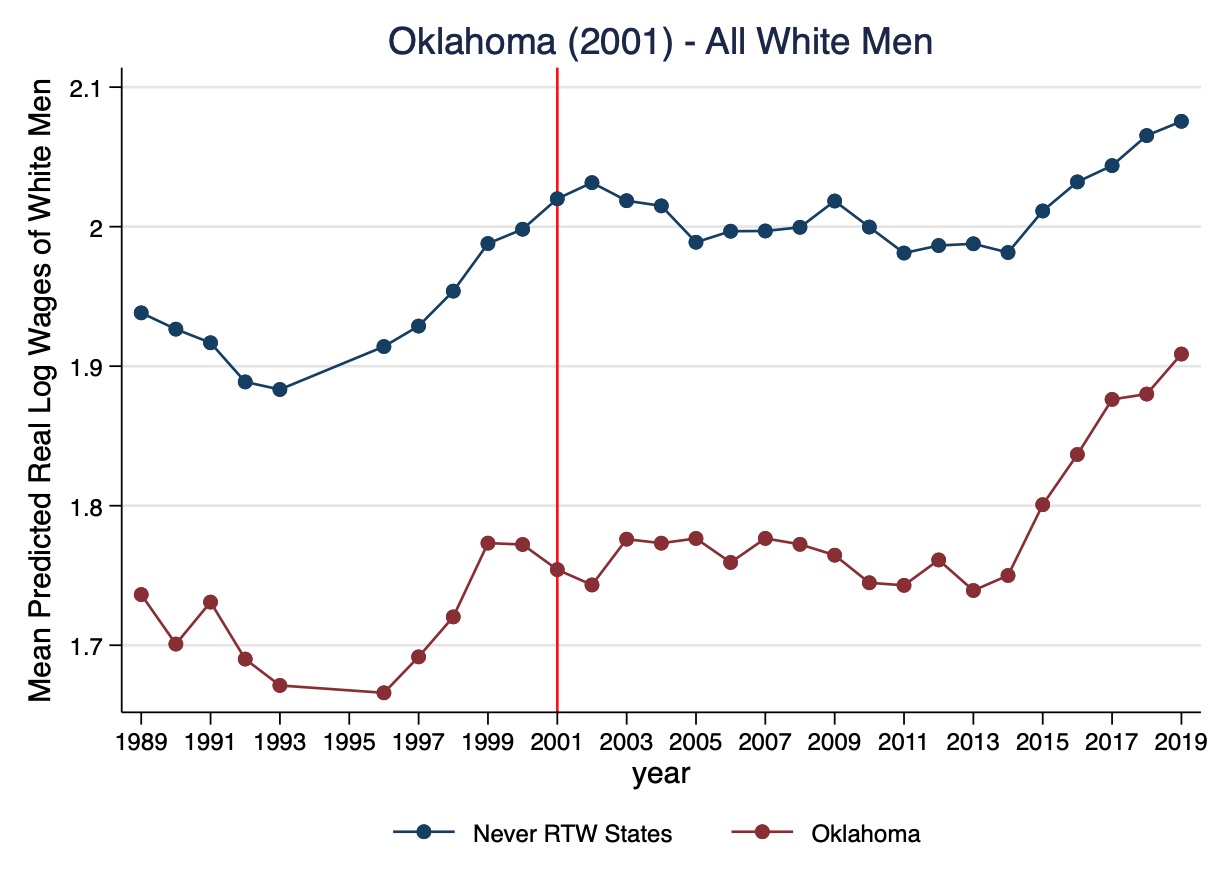
\includegraphics[width = 0.6\textwidth, keepaspectratio]{figures/pta/fin_wm_ok.png} & 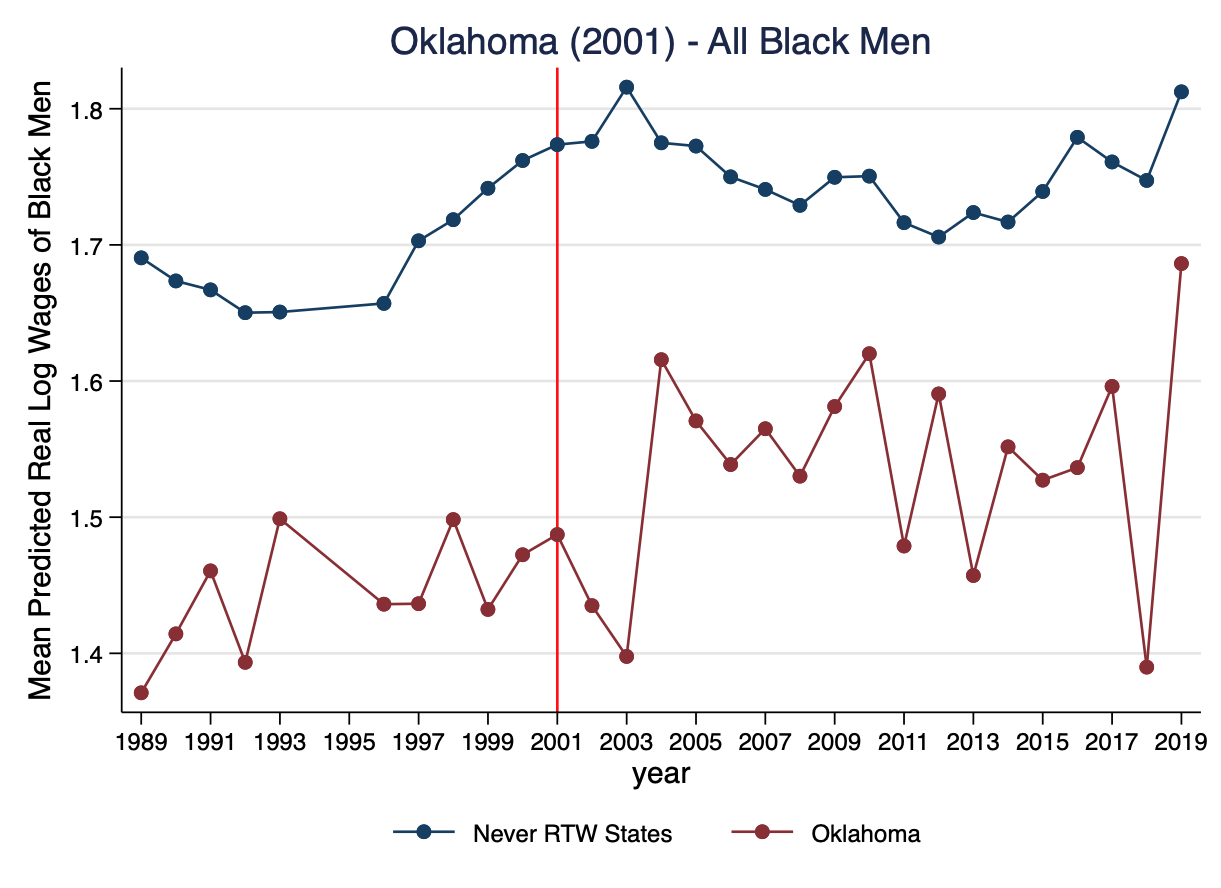
\includegraphics[width = 0.6\textwidth, keepaspectratio]{figures/pta/fin_bm_ok.png} \\
          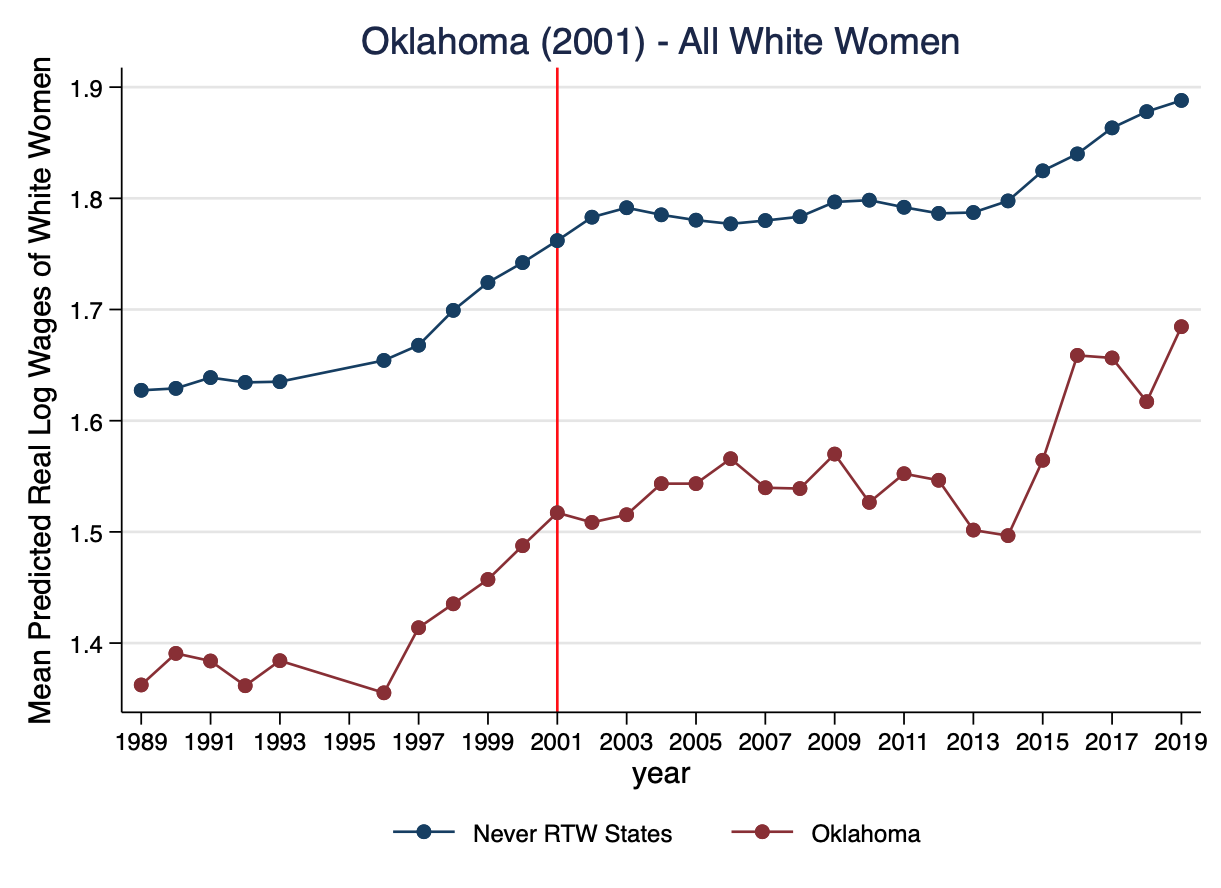
\includegraphics[width = 0.6\textwidth, keepaspectratio]{figures/pta/fin_wf_ok.png} & 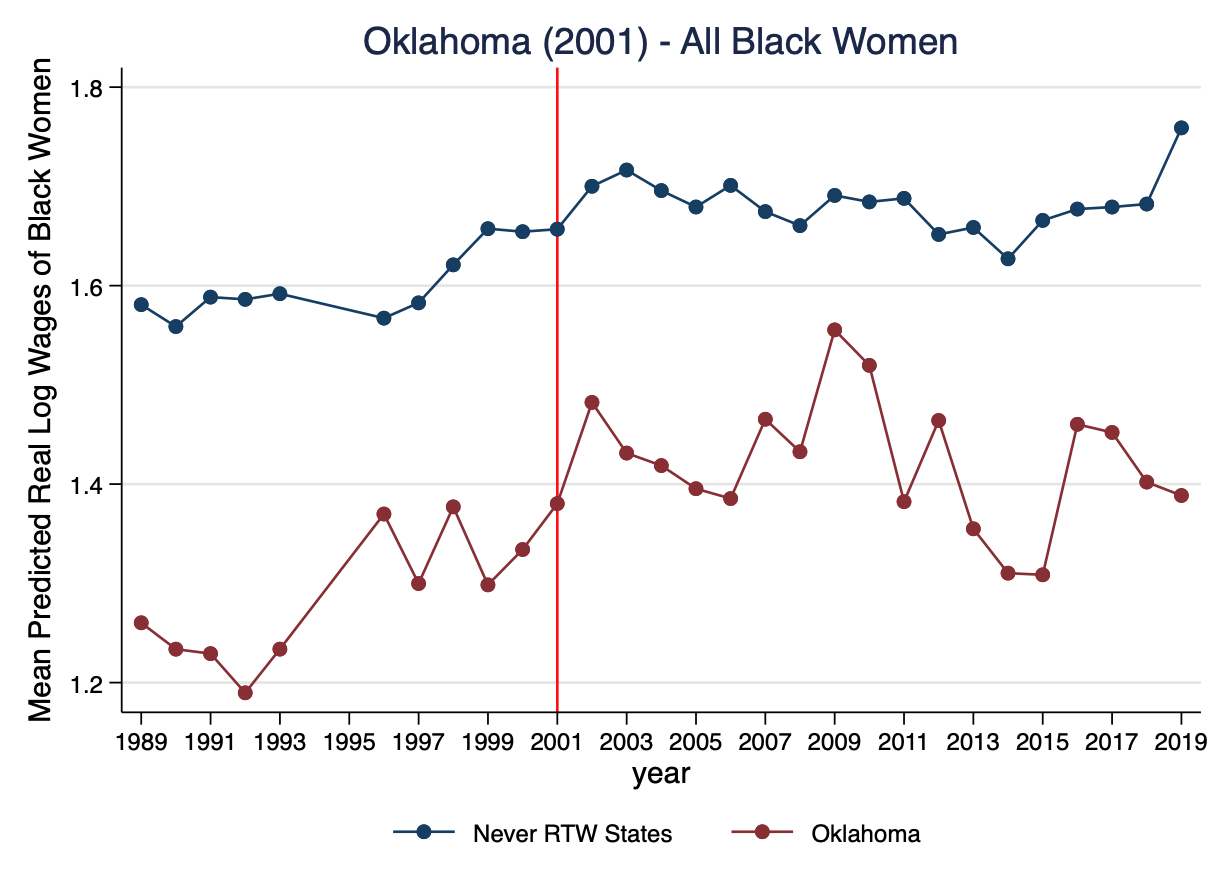
\includegraphics[width = 0.6\textwidth, keepaspectratio]{figures/pta/fin_bf_ok.png}
    \end{tabular}
\end{table}
% \footnotesize{Sample include years 1983-2019 excluding 1994 and 1995.}
\end{landscape}

\pagebreak
\begin{landscape}
\begin{table}[h!]
    \centering
    \captionof{figure}{Predicted Real Log Wage Trends - Indiana (2012)}\label{fig:pta_in}
    \begin{tabular}{c c}
          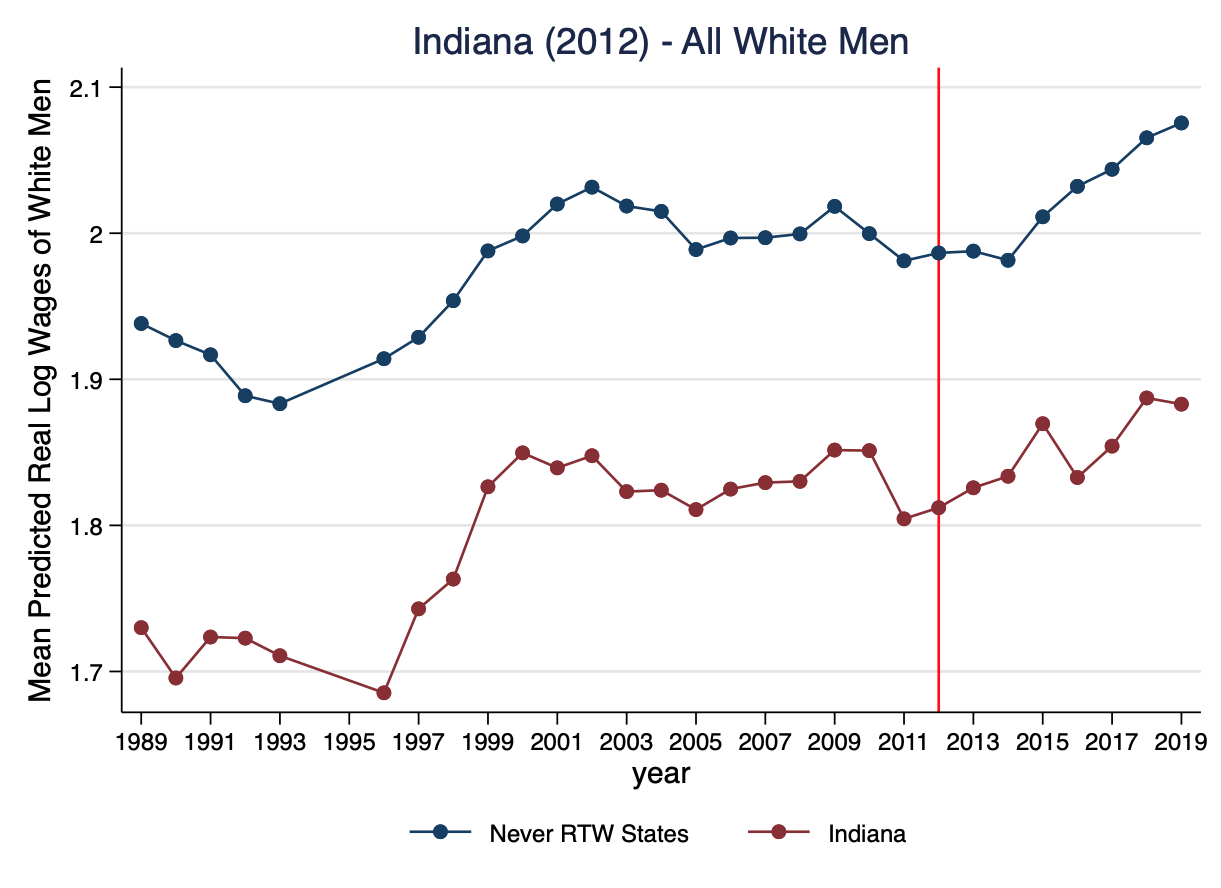
\includegraphics[width = 0.6\textwidth, keepaspectratio]{figures/pta/fin_wm_in.png} & 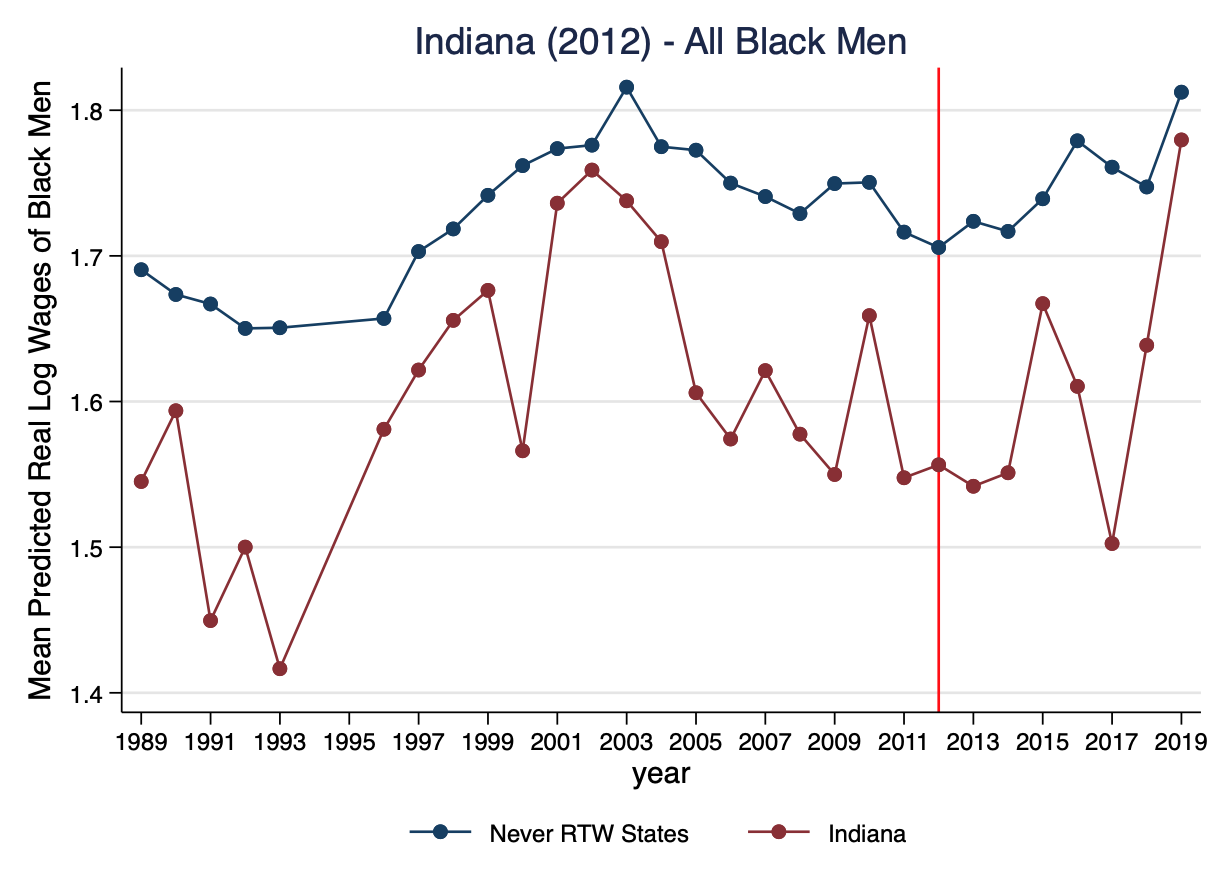
\includegraphics[width = 0.6\textwidth, keepaspectratio]{figures/pta/fin_bm_in.png} \\
          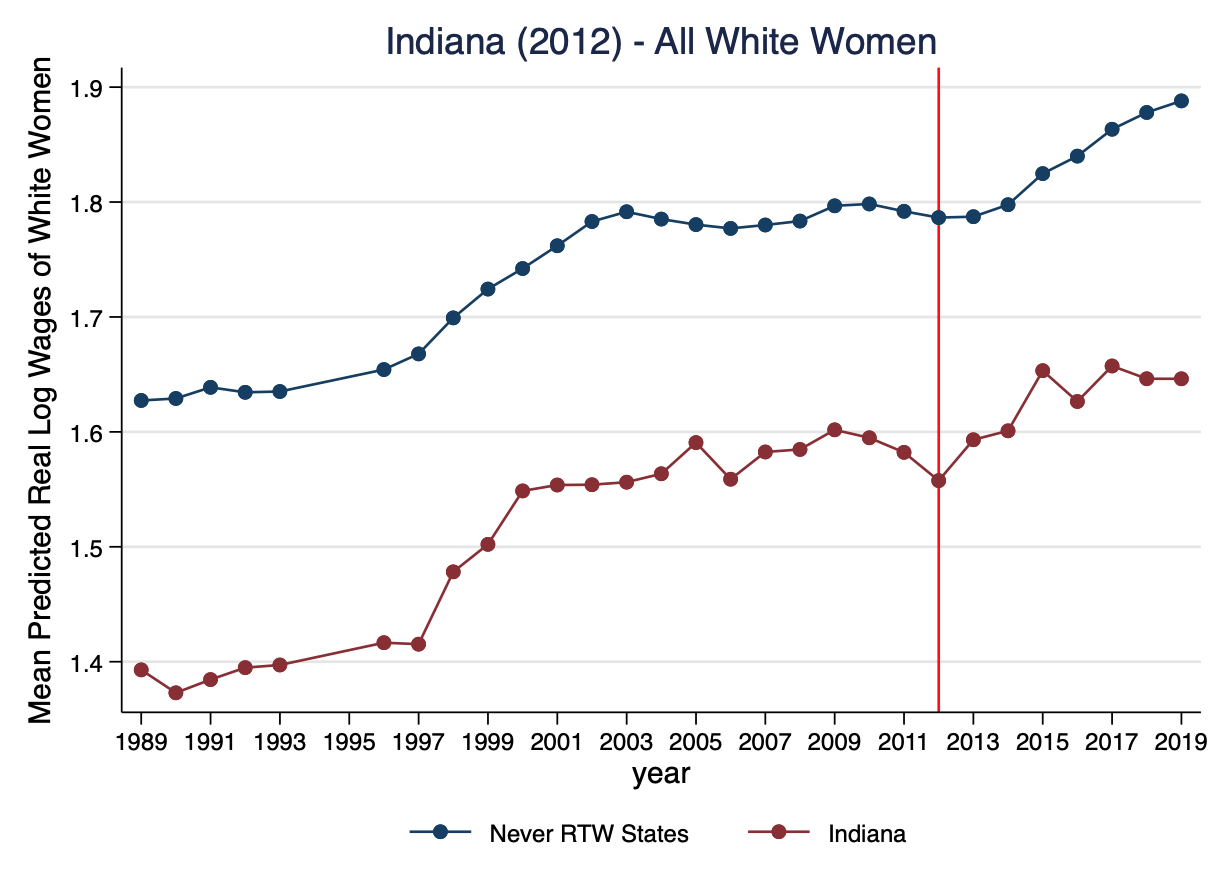
\includegraphics[width = 0.6\textwidth, keepaspectratio]{figures/pta/fin_wf_in.png} & 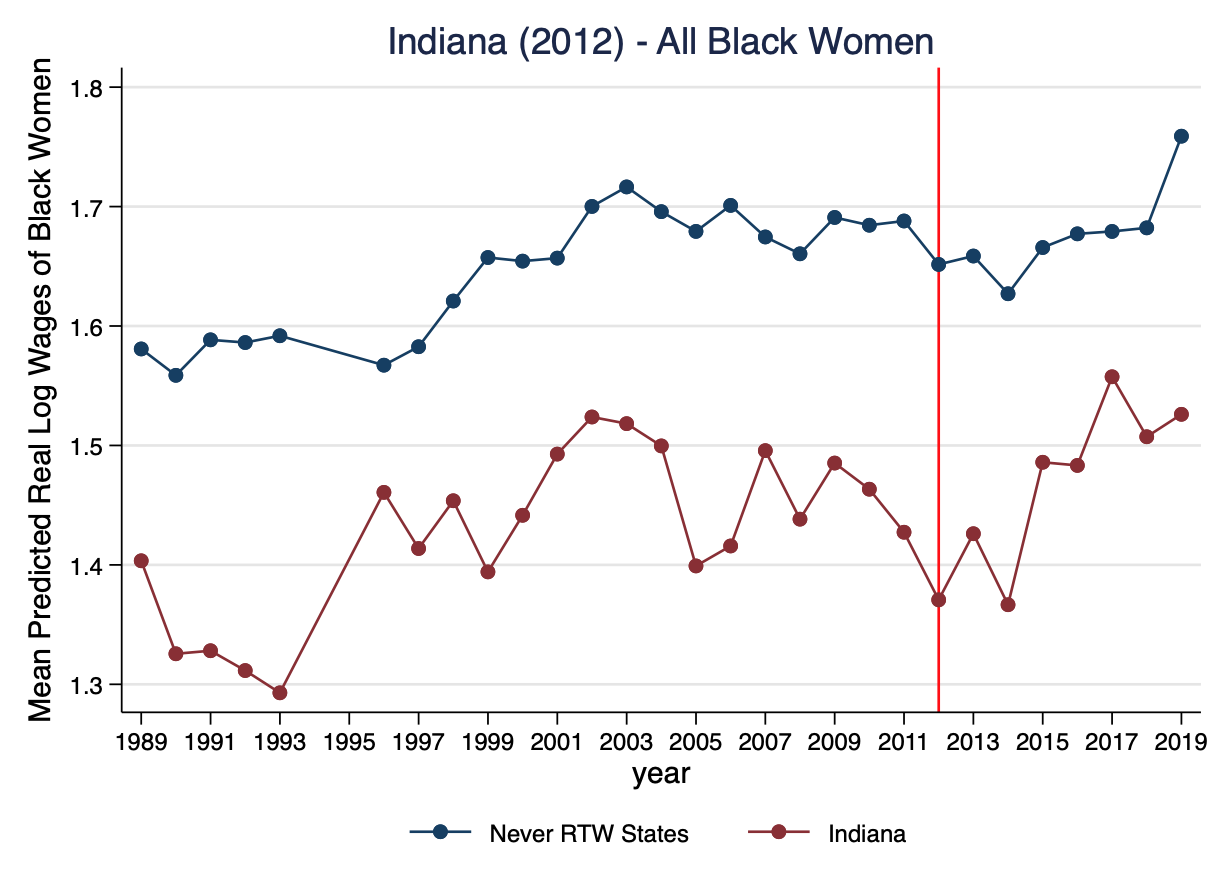
\includegraphics[width = 0.6\textwidth, keepaspectratio]{figures/pta/fin_bf_in.png}
    \end{tabular}
\end{table}
% \footnotesize{Sample include years 1983-2019 excluding 1994 and 1995.}
\end{landscape}

\pagebreak
\begin{landscape}
\begin{table}[h!]
    \centering
    \captionof{figure}{Predicted Real Log Wage Trends - Michigan (2013)}\label{fig:pta_mi}
    \begin{tabular}{c c}
          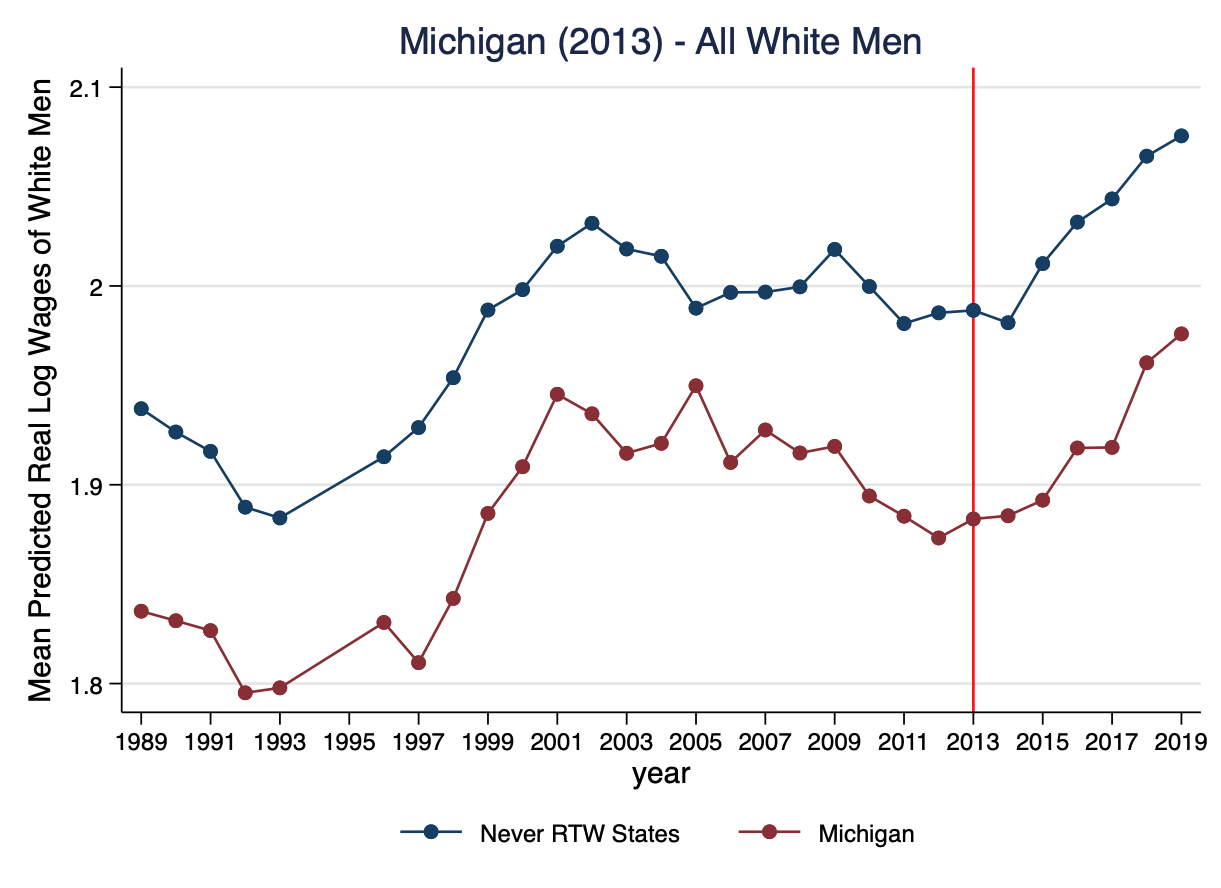
\includegraphics[width = 0.6\textwidth, keepaspectratio]{figures/pta/fin_wm_mi.png} & 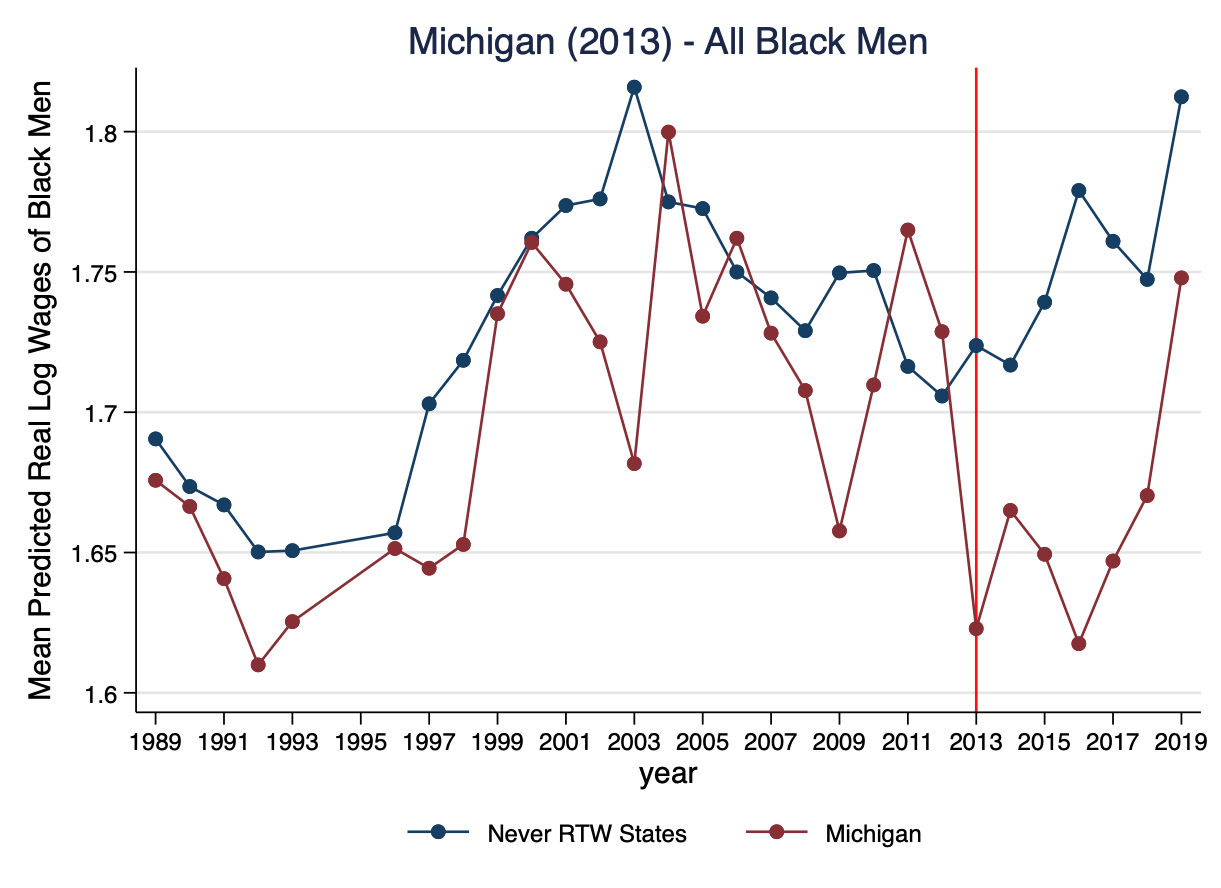
\includegraphics[width = 0.6\textwidth, keepaspectratio]{figures/pta/fin_bm_mi.png} \\
          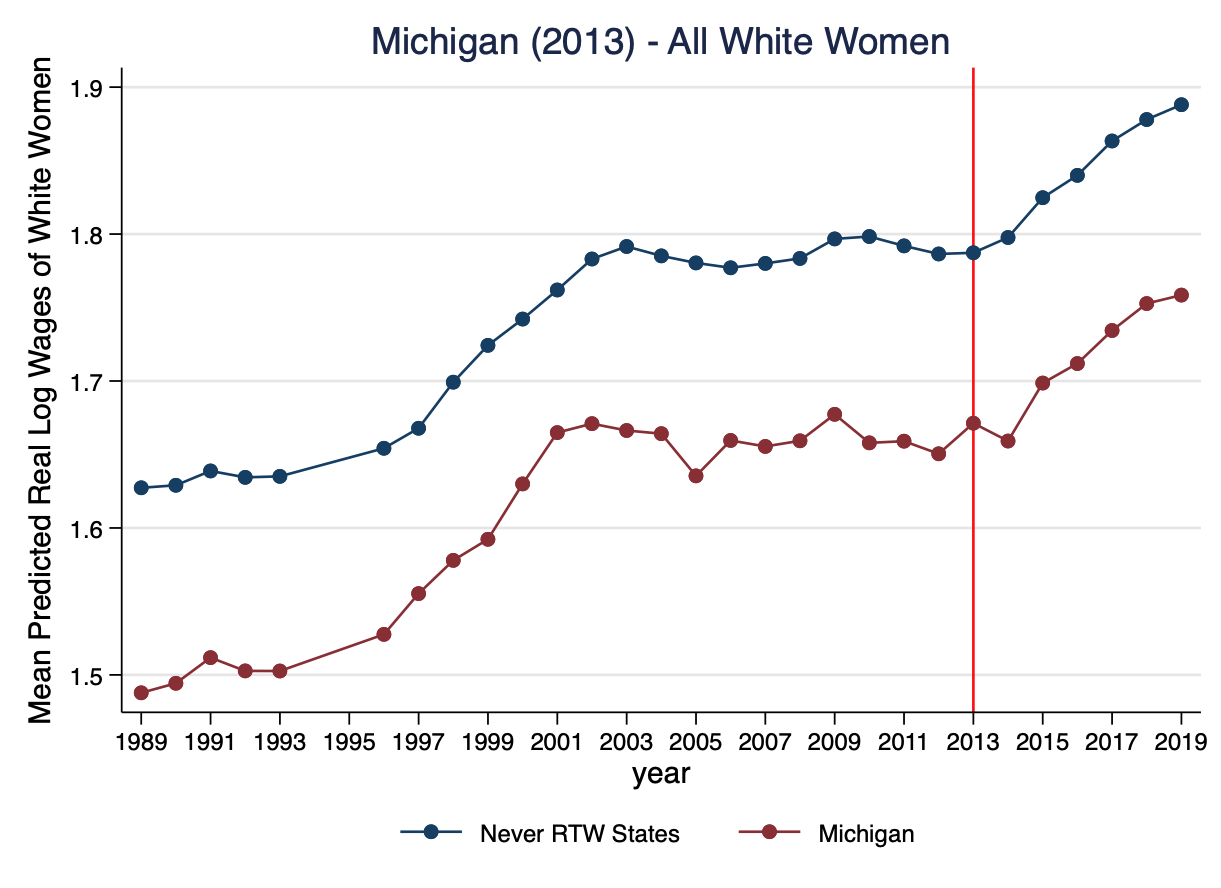
\includegraphics[width = 0.6\textwidth, keepaspectratio]{figures/pta/fin_wf_mi.png} & 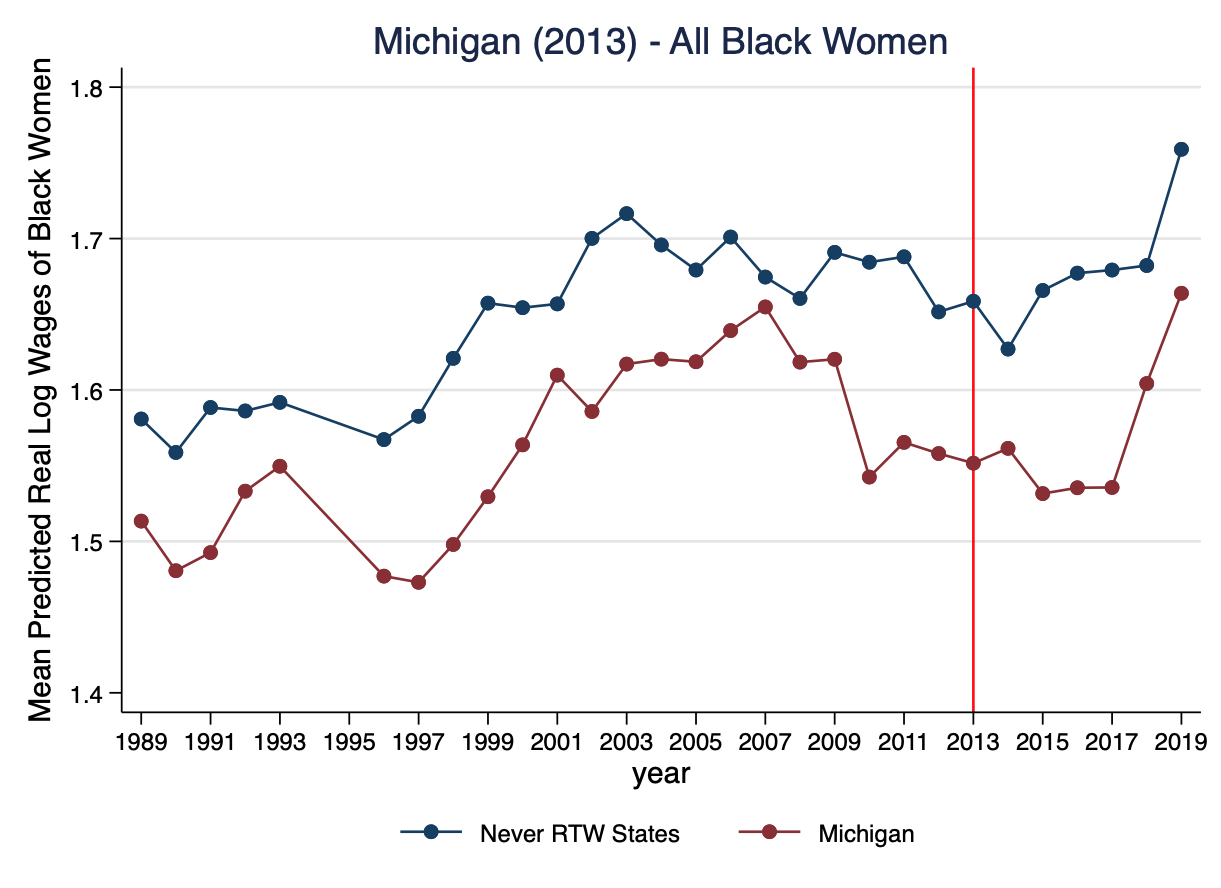
\includegraphics[width = 0.6\textwidth, keepaspectratio]{figures/pta/fin_bf_mi.png}
    \end{tabular}
\end{table}
% \footnotesize{Sample include years 1983-2019 excluding 1994 and 1995.}
\end{landscape}

\pagebreak
\begin{landscape}
\begin{table}[h!]
    \centering
    \captionof{figure}{Predicted Real Log Wage Trends - Wisconsin (2015)}\label{fig:pta_wi}
    \begin{tabular}{c c}
          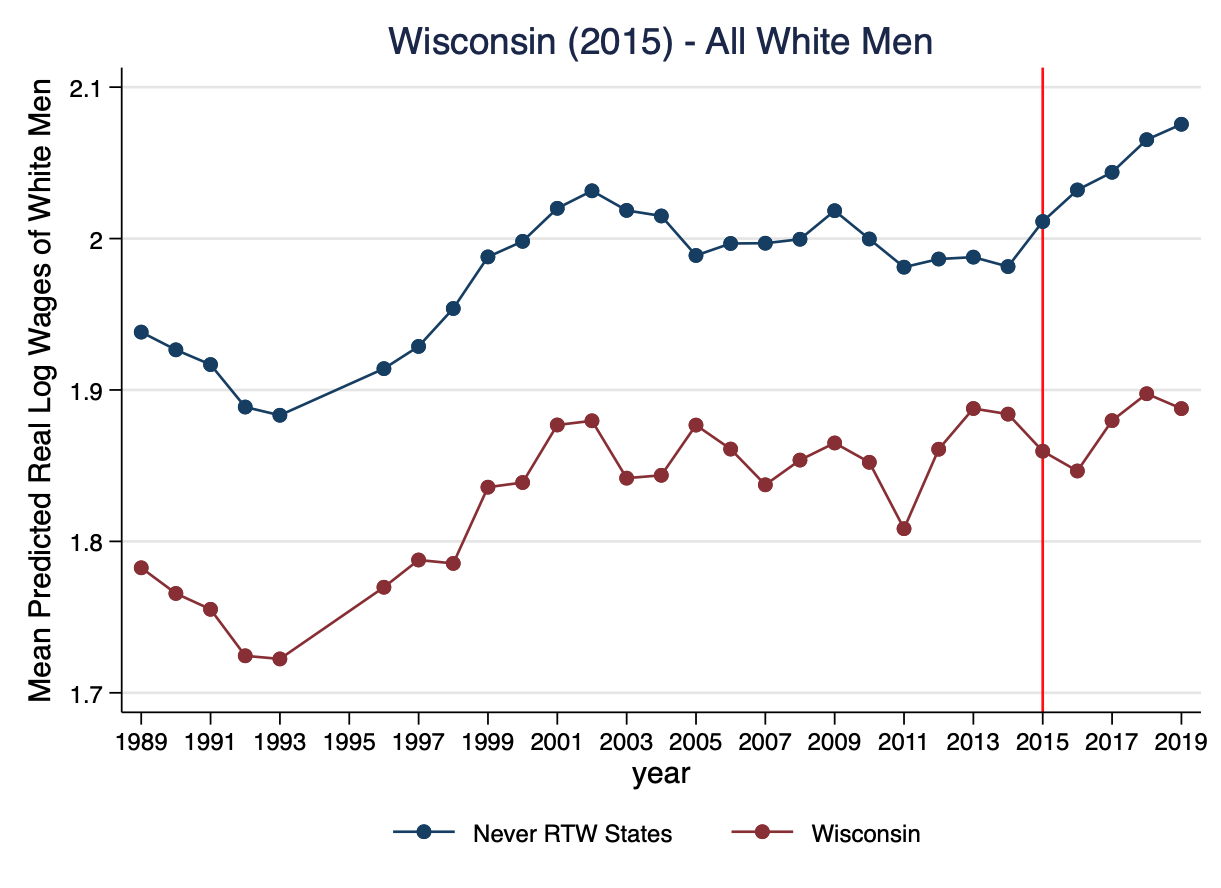
\includegraphics[width = 0.6\textwidth, keepaspectratio]{figures/pta/fin_wm_wi.png} & 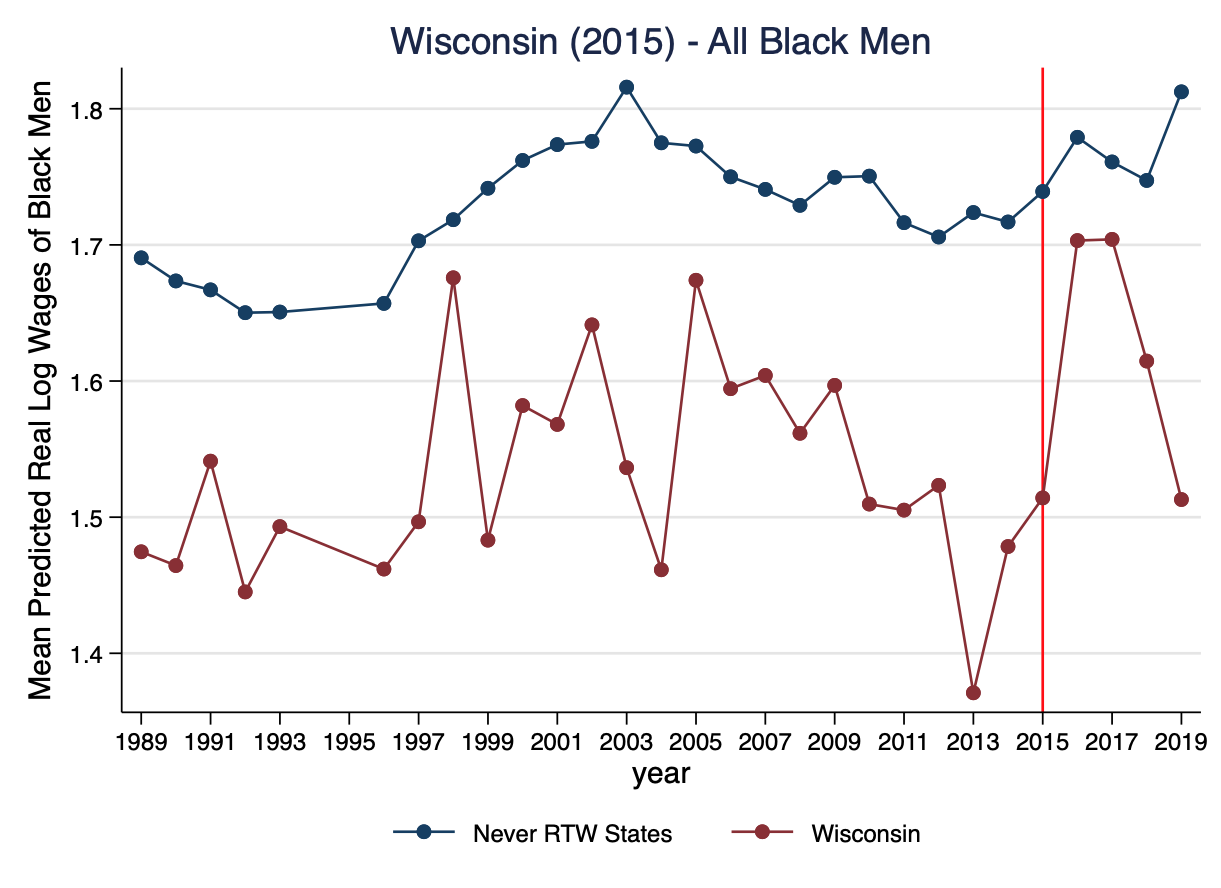
\includegraphics[width = 0.6\textwidth, keepaspectratio]{figures/pta/fin_bm_wi.png} \\
          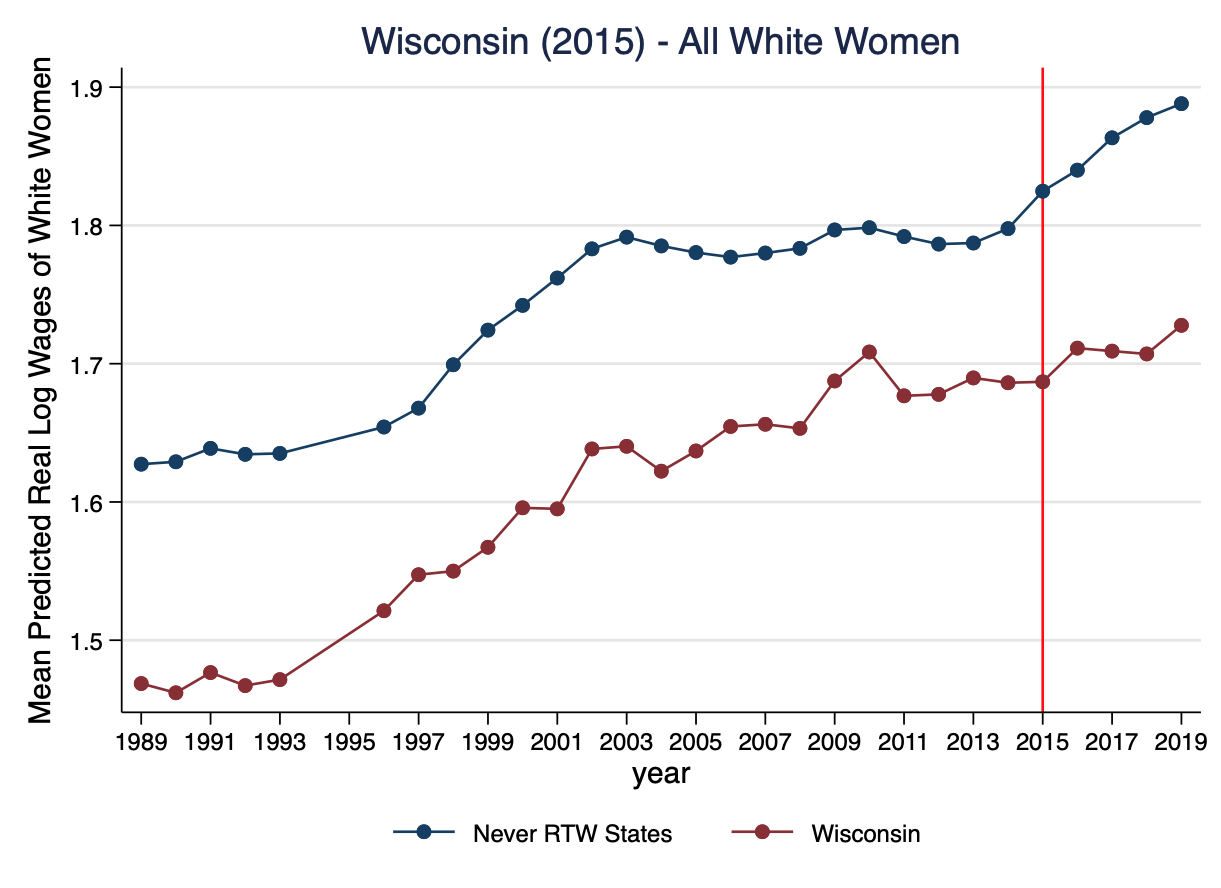
\includegraphics[width = 0.6\textwidth, keepaspectratio]{figures/pta/fin_wf_wi.png} & 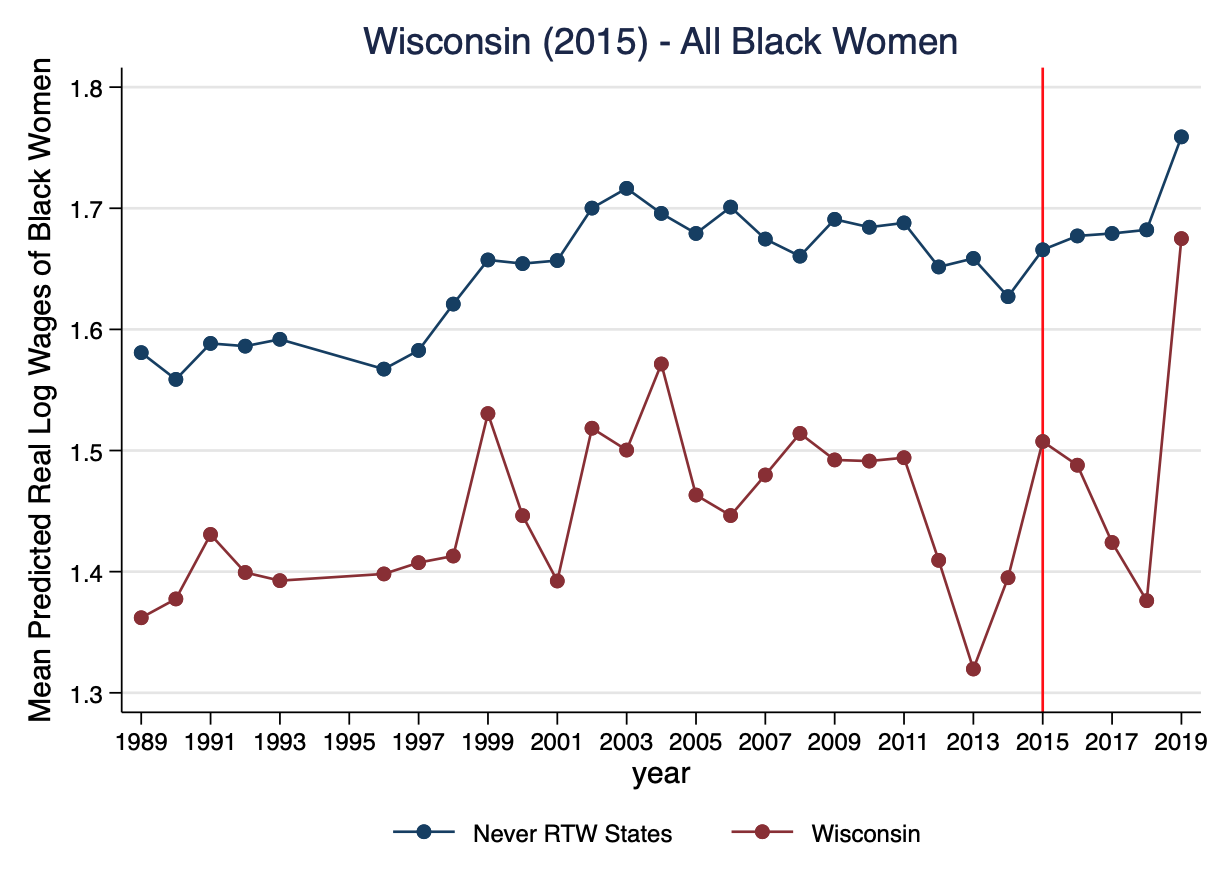
\includegraphics[width = 0.6\textwidth, keepaspectratio]{figures/pta/fin_bf_wi.png}
    \end{tabular}
\end{table}
% \footnotesize{Sample include years 1983-2019 excluding 1994 and 1995.}
\end{landscape}

\pagebreak
\begin{landscape}
\begin{table}[h!]
    \centering
    \captionof{figure}{Predicted Real Log Wage Trends - Kentucky (2017)}\label{fig:pta_ky}
    \begin{tabular}{c c}
          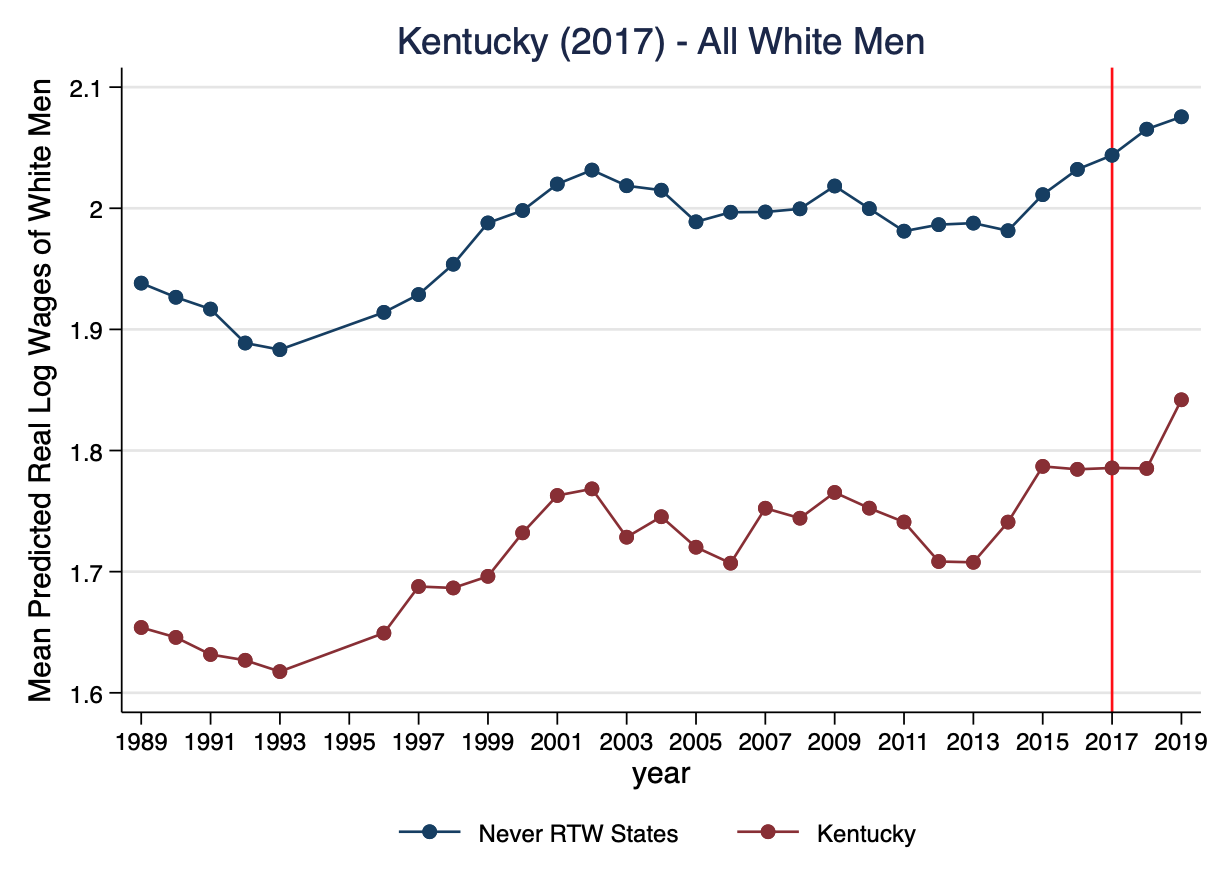
\includegraphics[width = 0.6\textwidth, keepaspectratio]{figures/pta/fin_wm_ky.png} & 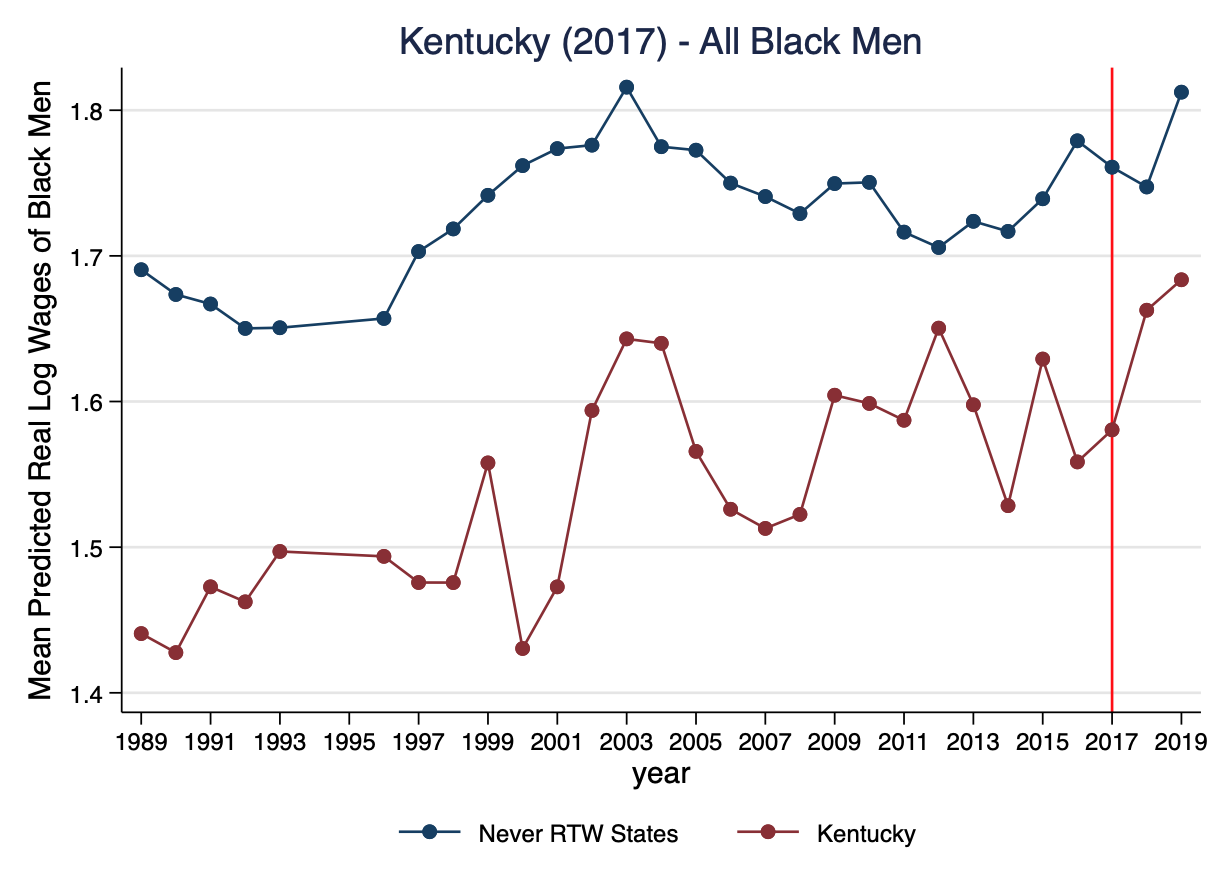
\includegraphics[width = 0.6\textwidth, keepaspectratio]{figures/pta/fin_bm_ky.png} \\
          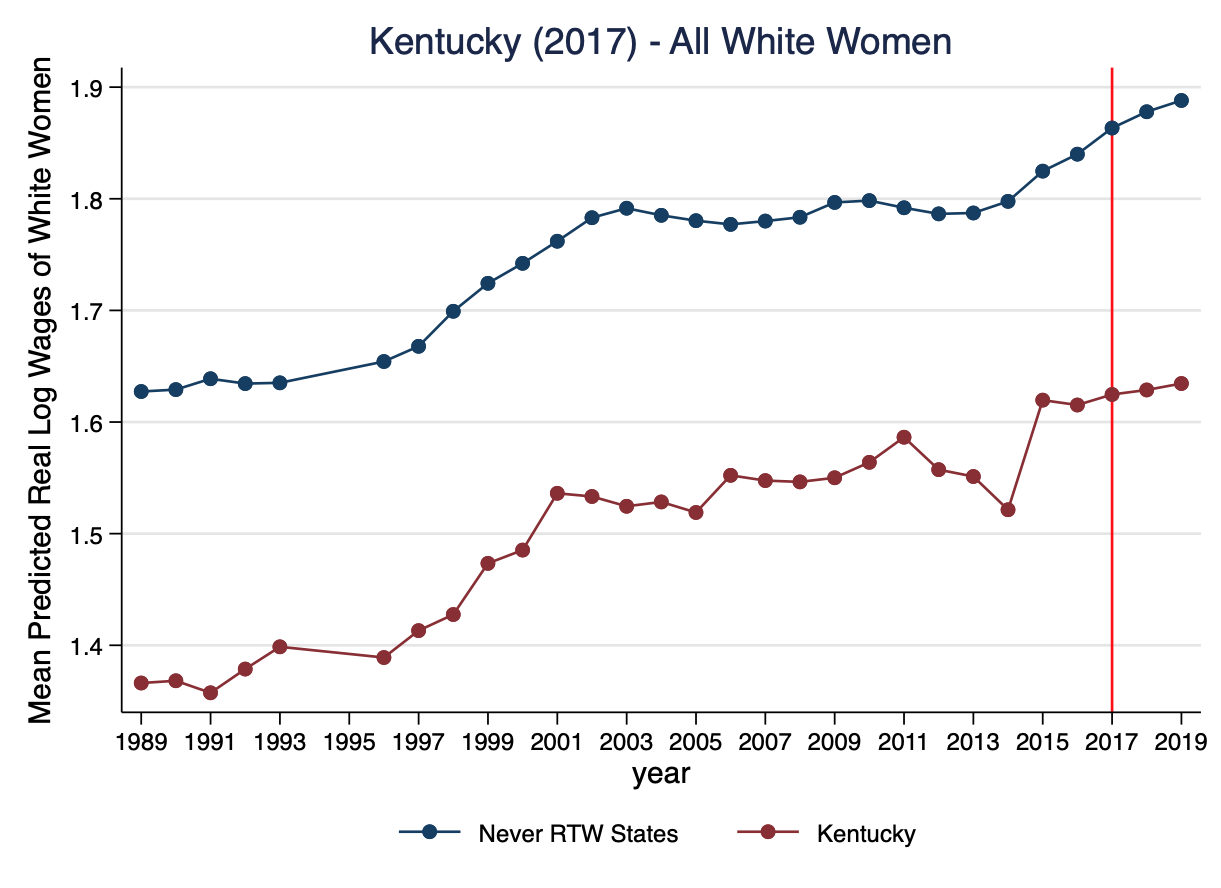
\includegraphics[width = 0.6\textwidth, keepaspectratio]{figures/pta/fin_wf_ky.png} & 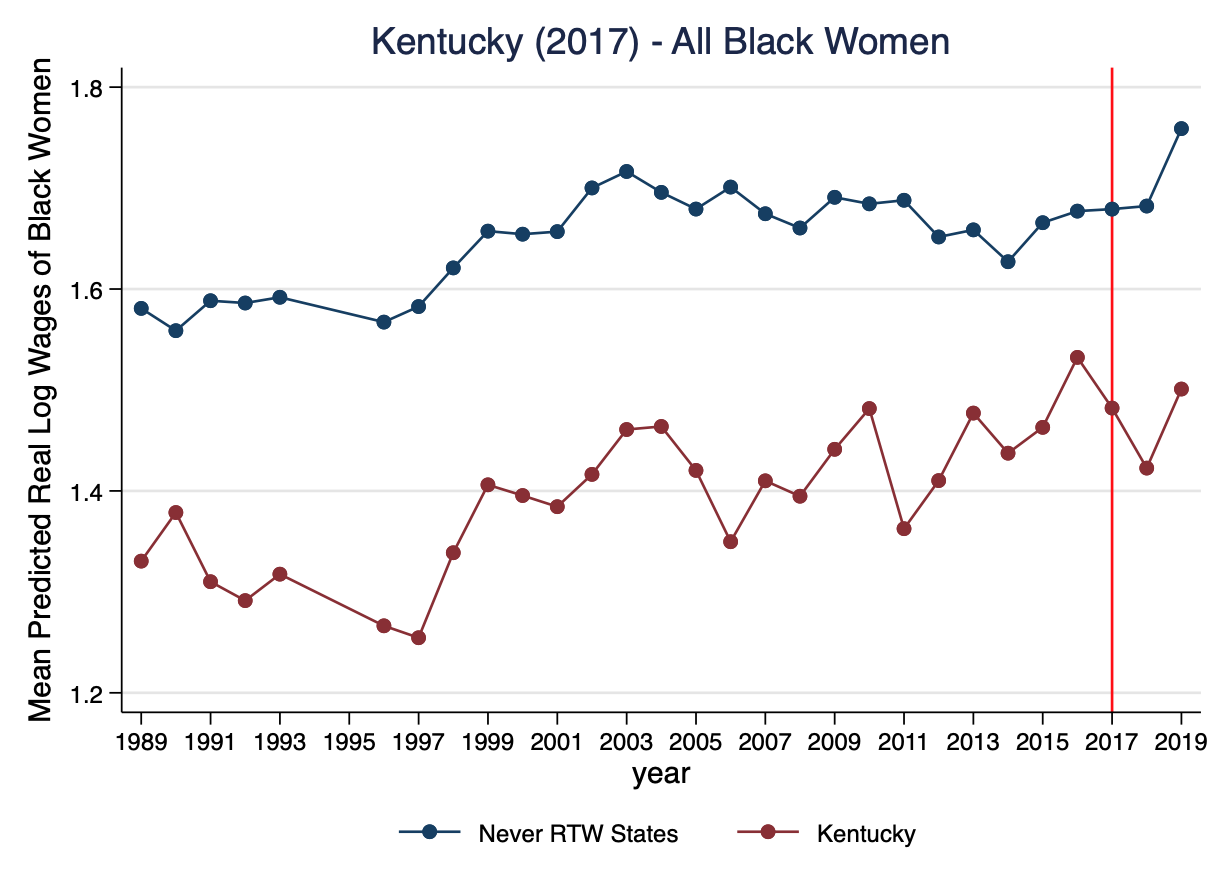
\includegraphics[width = 0.6\textwidth, keepaspectratio]{figures/pta/fin_bf_ky.png}
    \end{tabular}
\end{table}
% \footnotesize{Sample include years 1983-2019 excluding 1994 and 1995.}
\end{landscape}

\pagebreak
\begin{landscape}
\begin{table}[ht!]
    \centering
    \captionof{figure}{Synthetic Control Method - Oklahoma (2001)}\label{fig:synth_ok}
    \begin{tabular}{c c}
          \textbf{White Men} & \textbf{Black Men} \\
          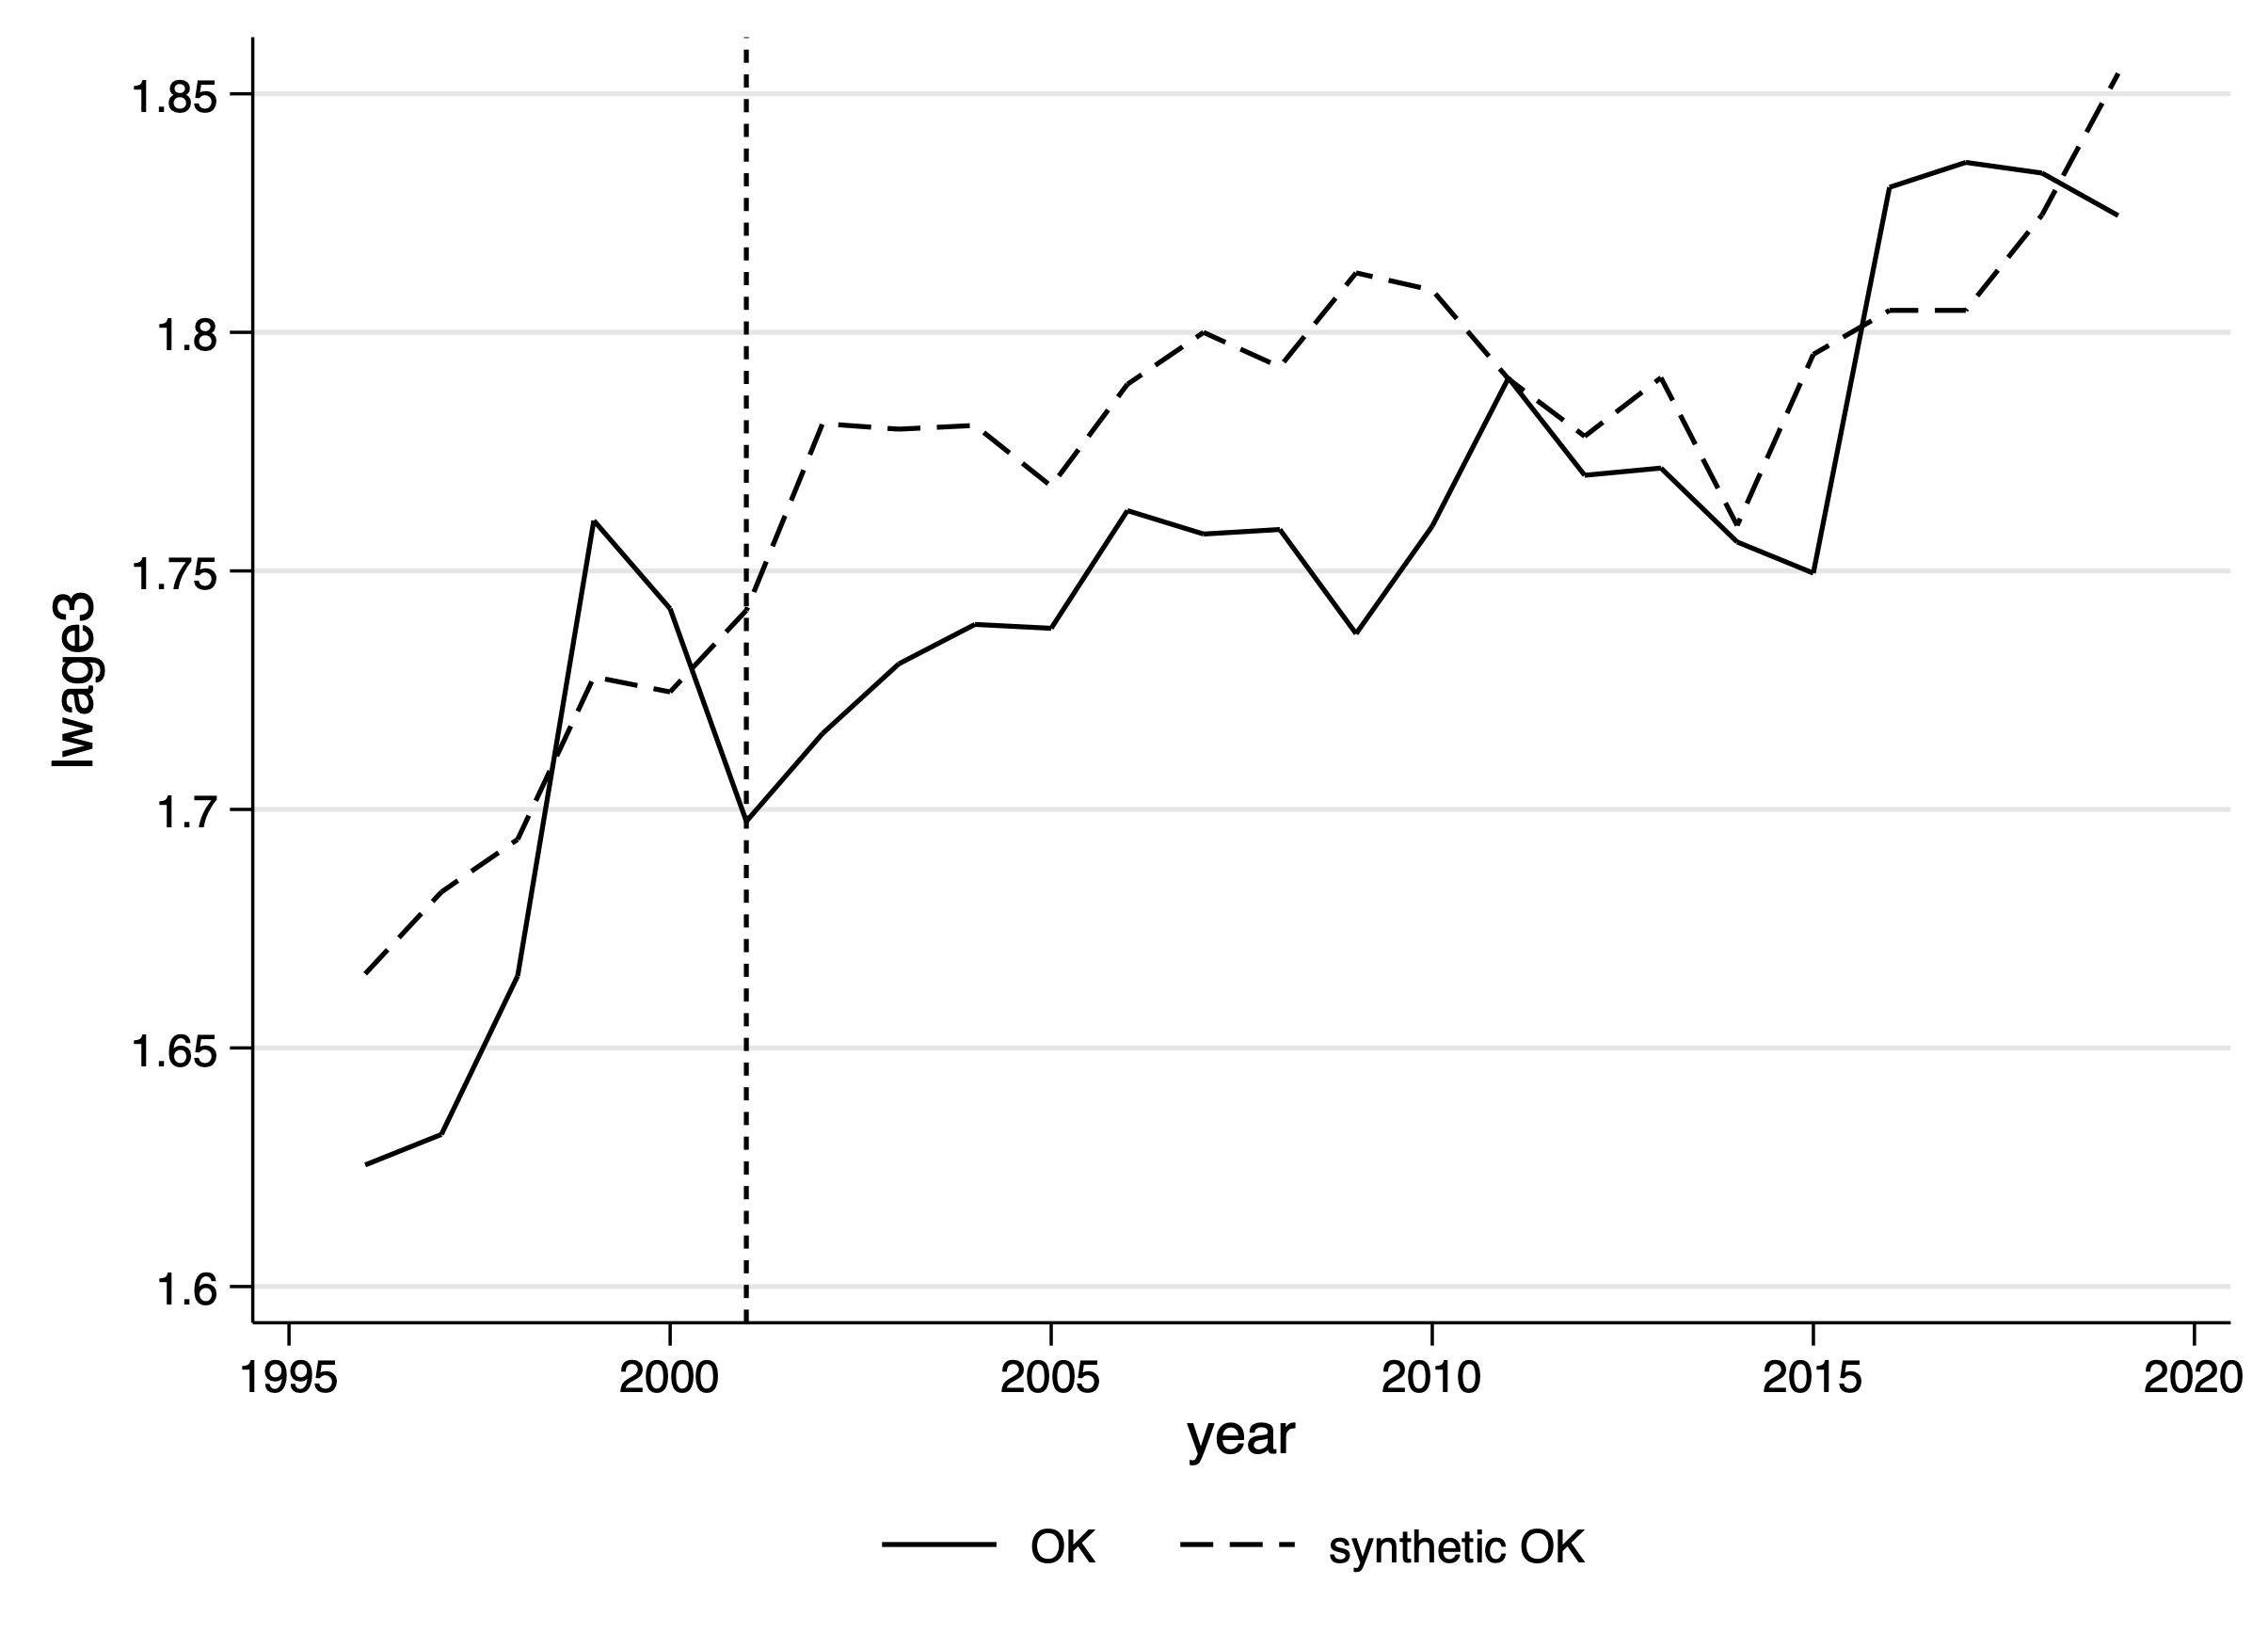
\includegraphics[width = 0.6\textwidth, keepaspectratio]{figures/fin_synth_wm_ok.png} & 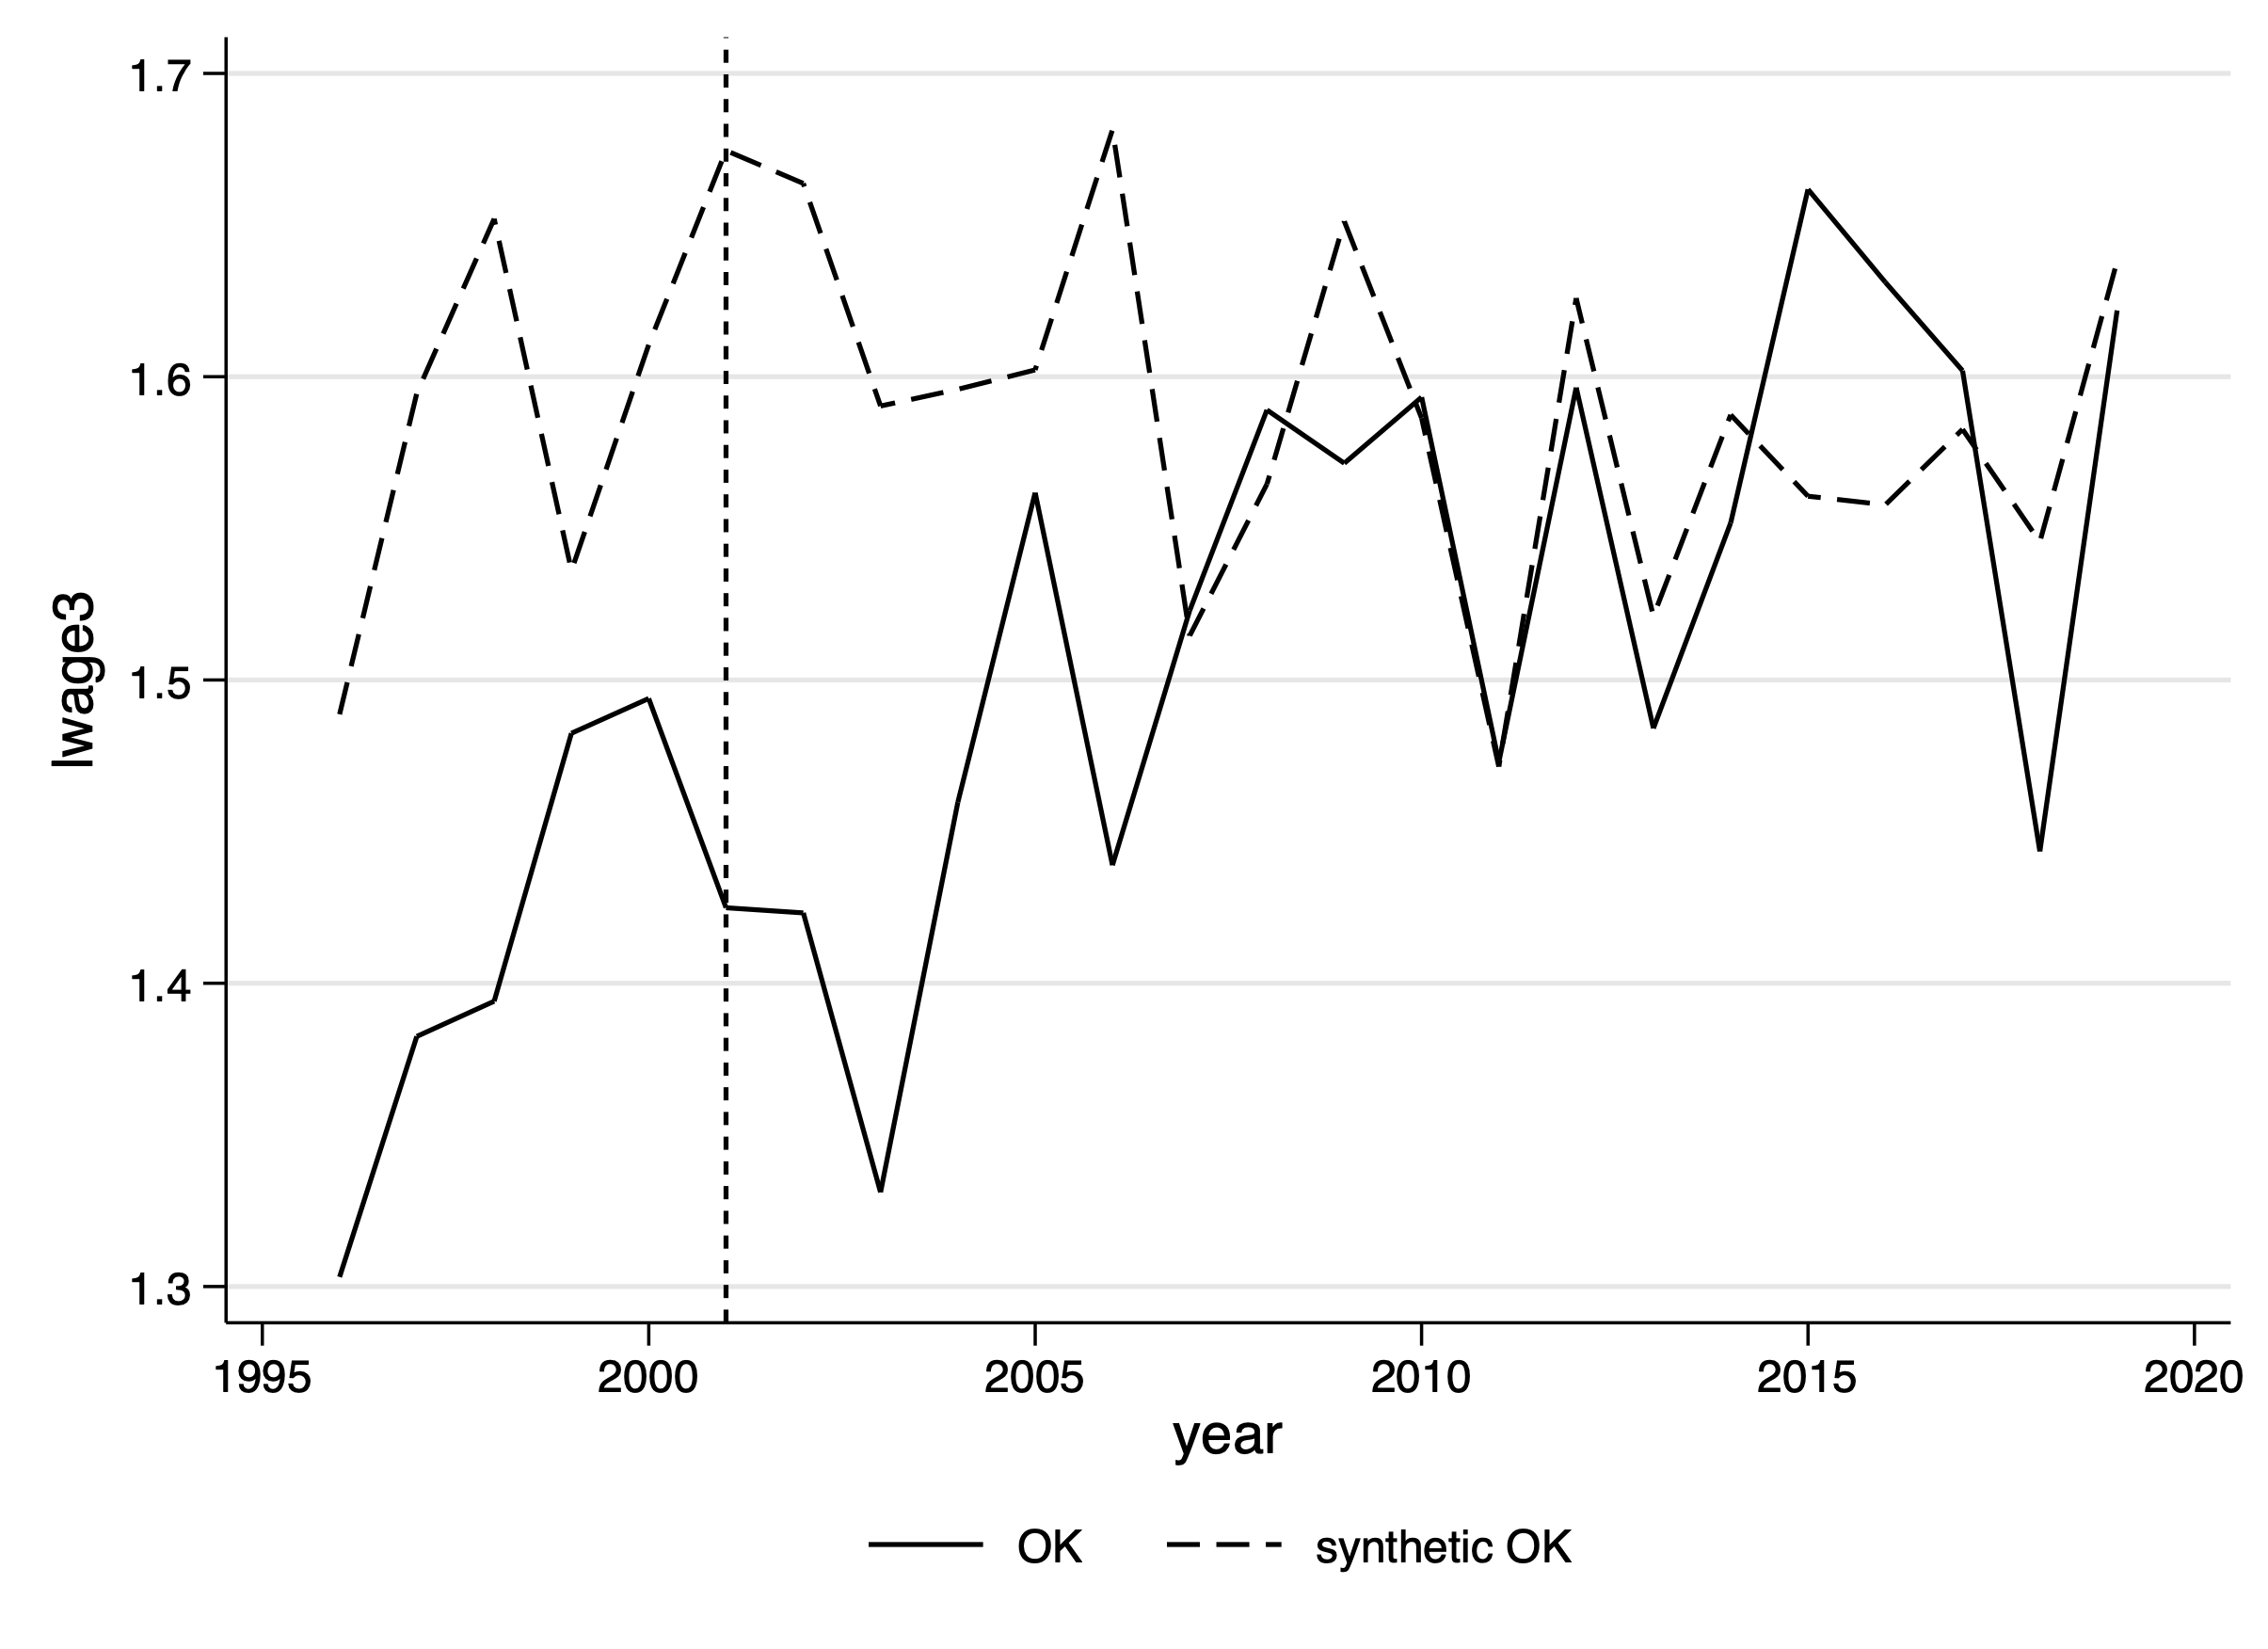
\includegraphics[width = 0.6\textwidth, keepaspectratio]{figures/fin_synth_bm_ok.png} \\
          \textbf{White Women} & \textbf{Black Women} \\
          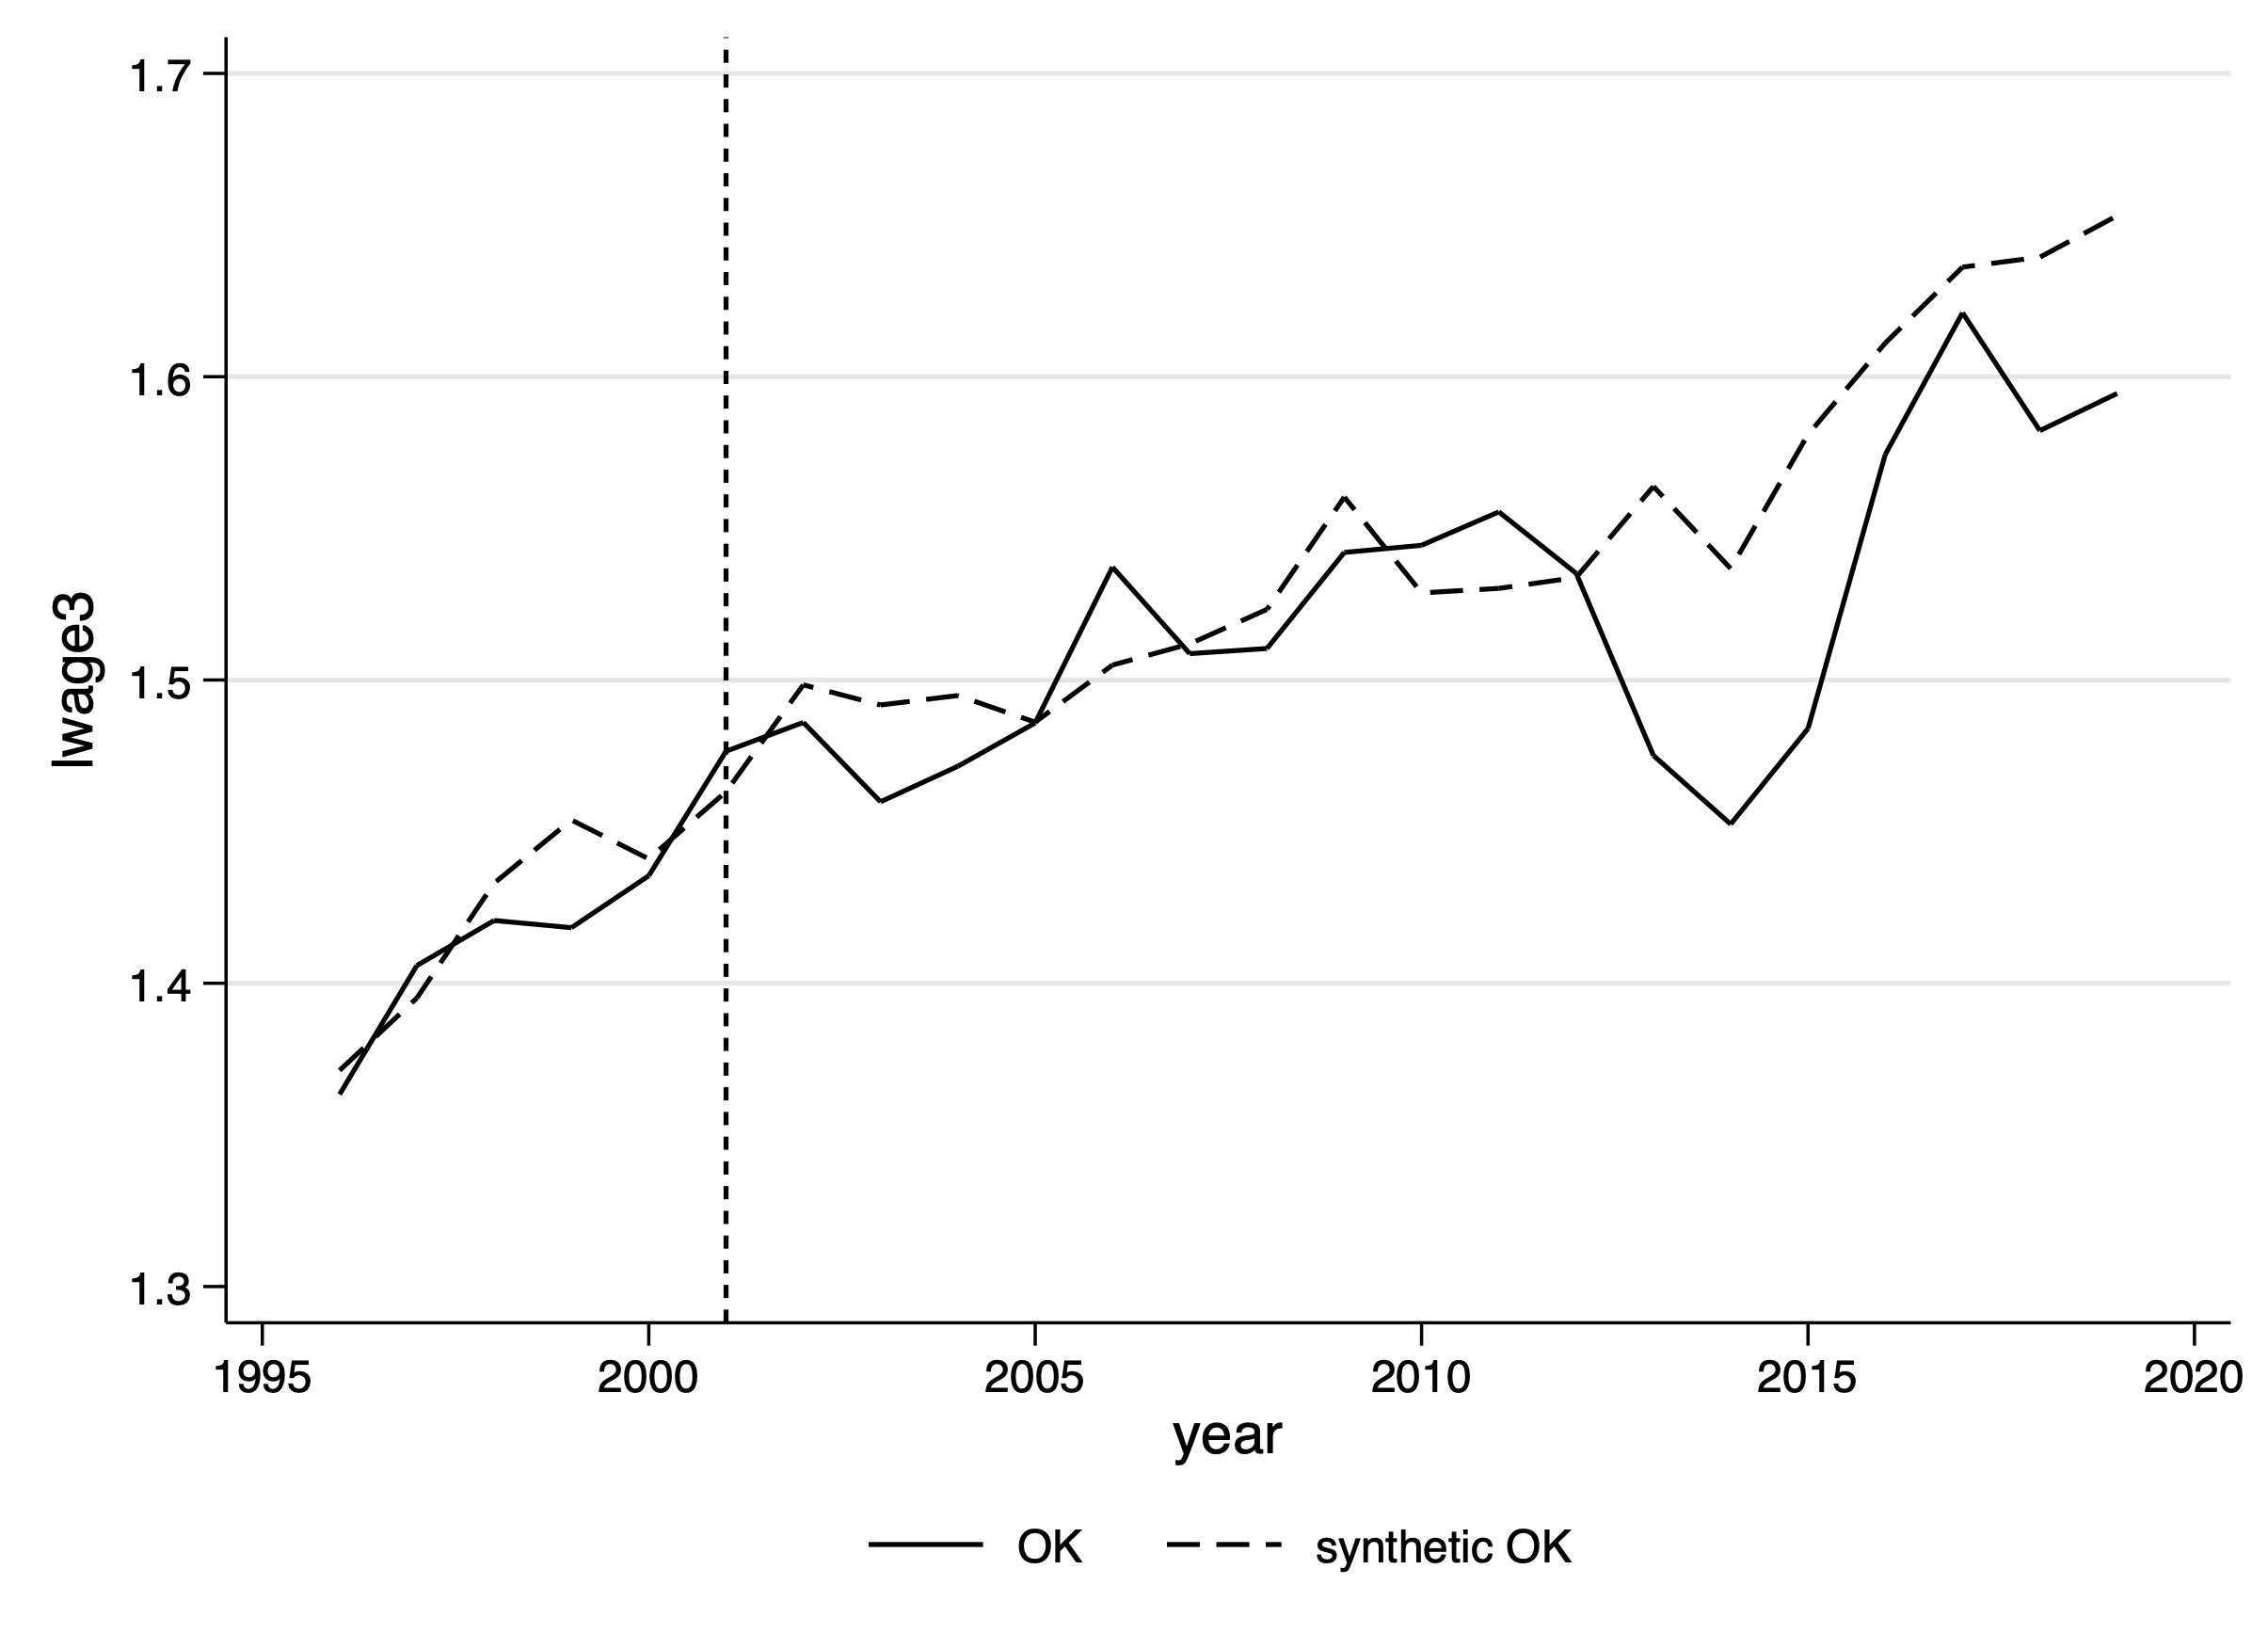
\includegraphics[width = 0.6\textwidth, keepaspectratio]{figures/fin_synth_wf_ok.png} & 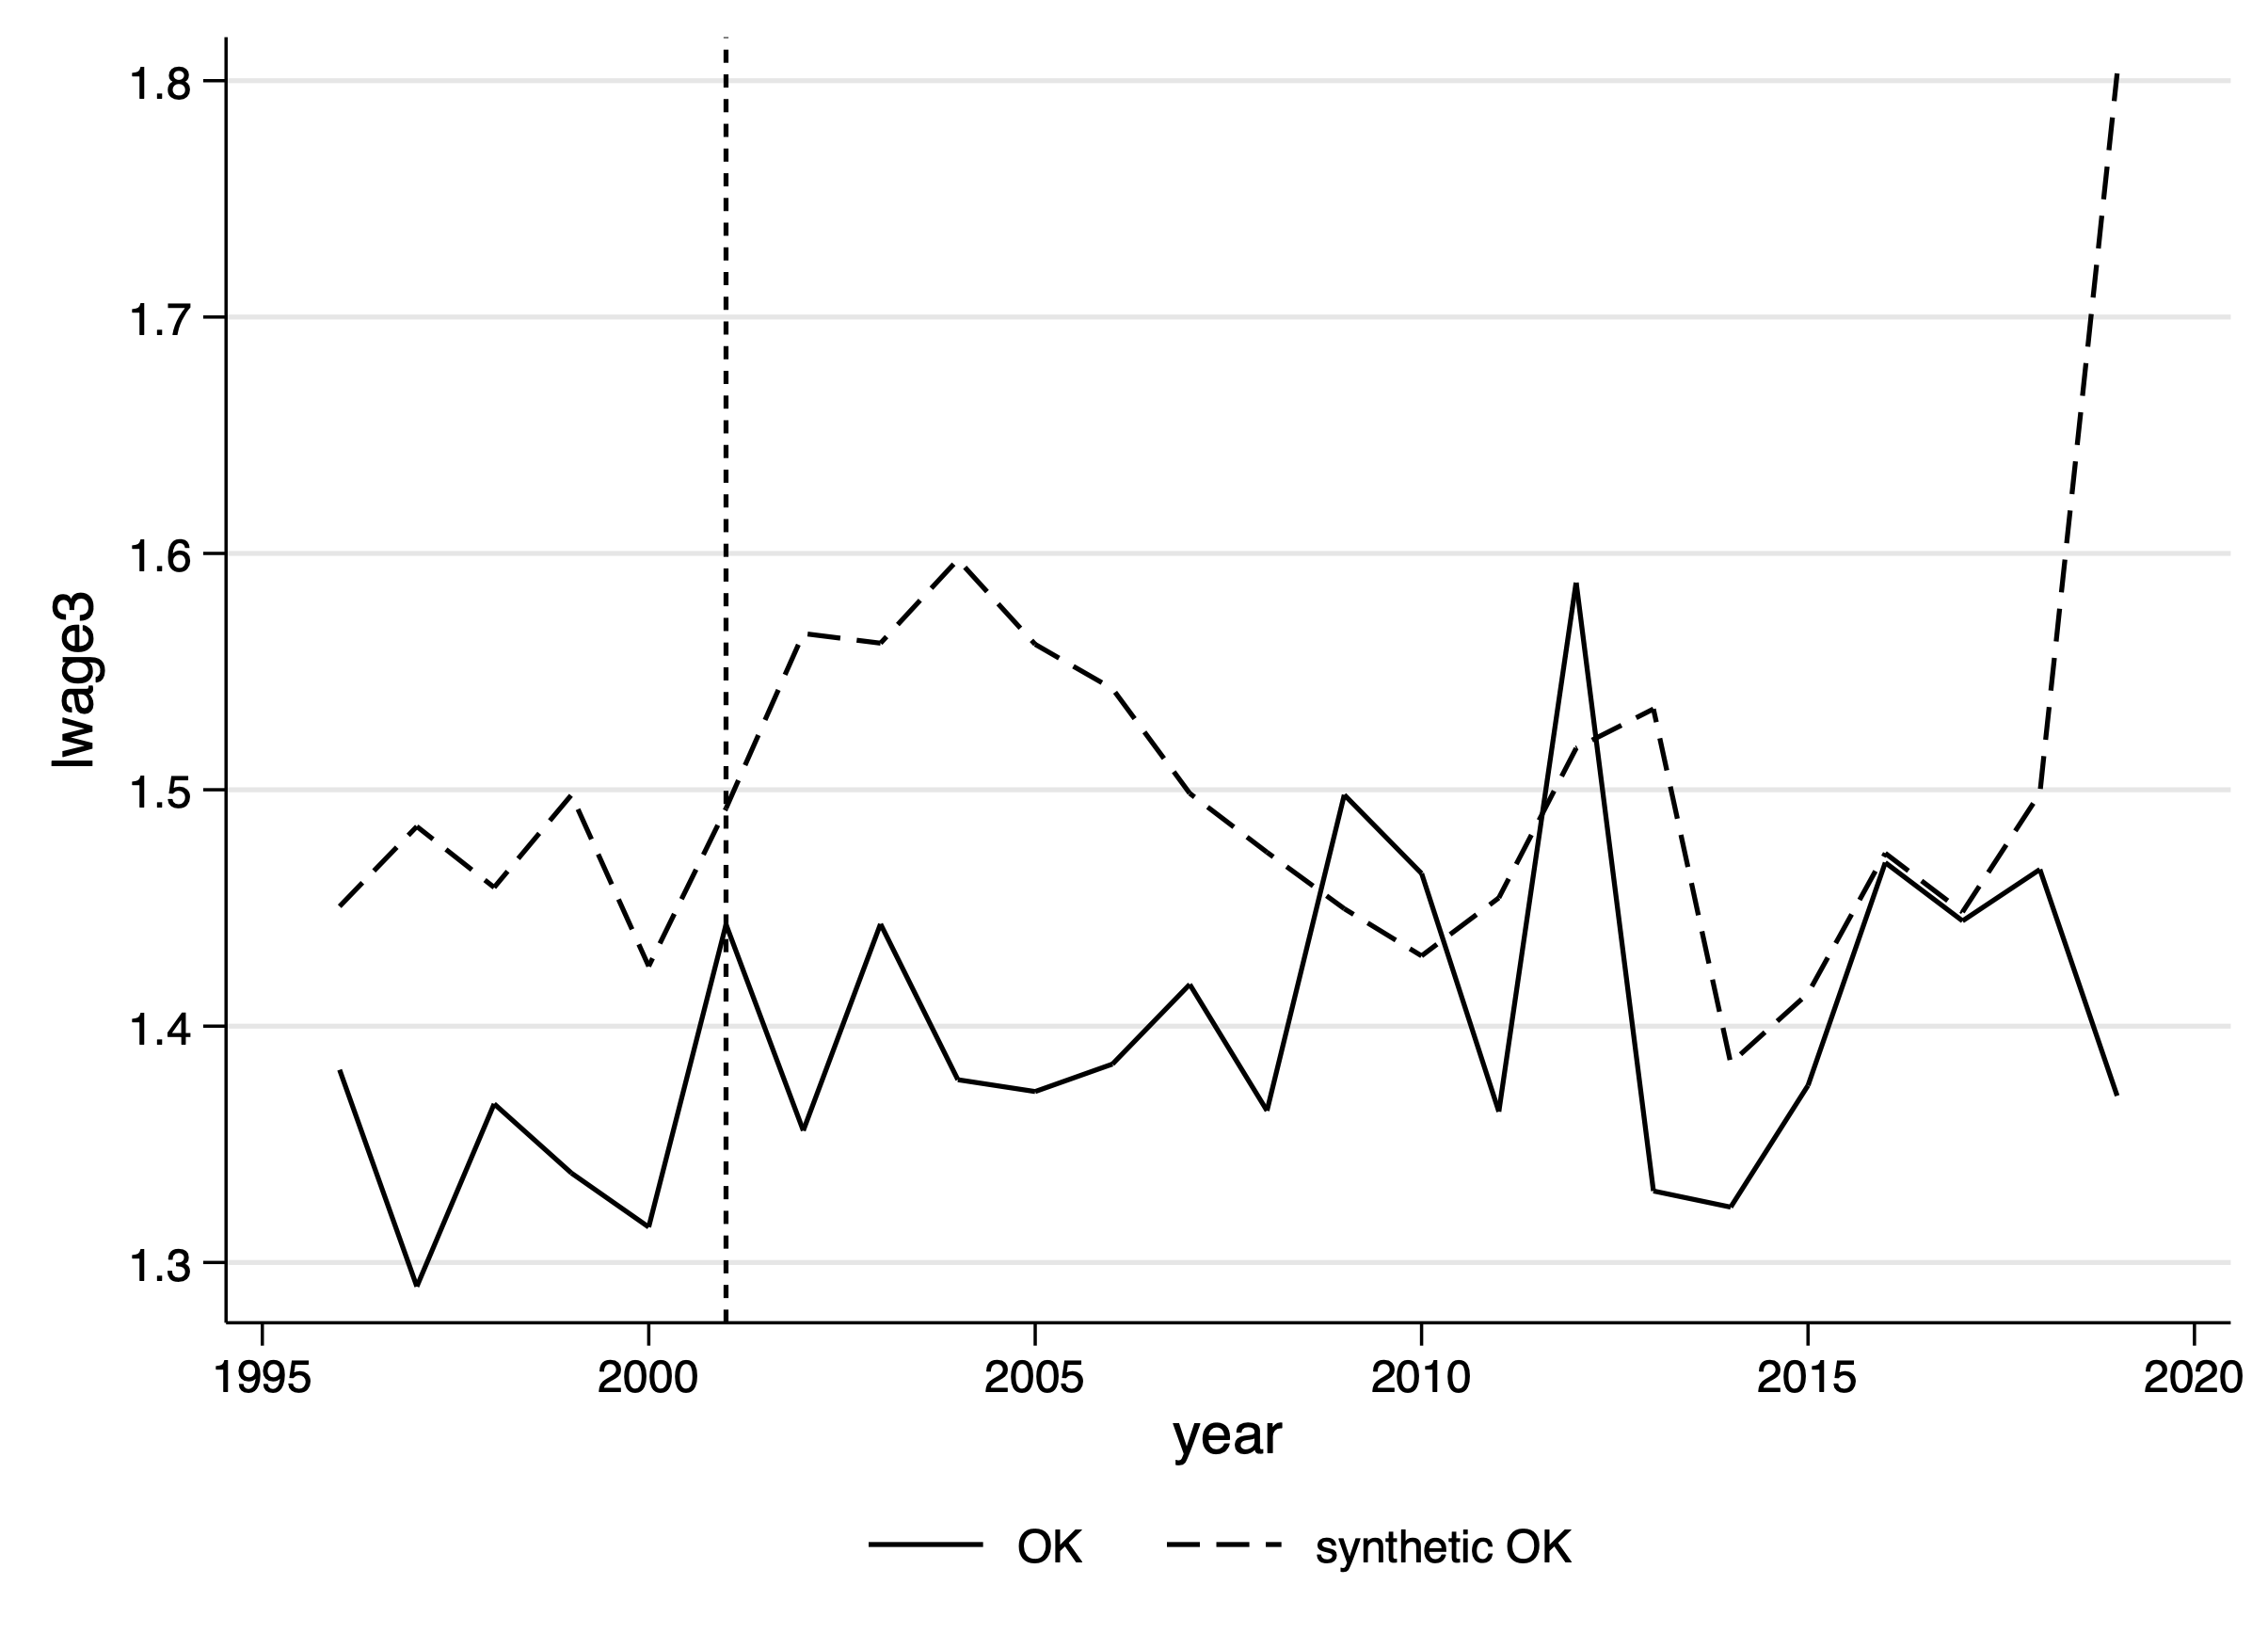
\includegraphics[width = 0.6\textwidth, keepaspectratio]{figures/fin_synth_bf_ok.png}
    \end{tabular}
\end{table}
% \footnotesize{Sample include years 1983-2019 excluding 1994 and 1995.}
\end{landscape}

\pagebreak
\begin{landscape}
\begin{table}[ht!]
    \centering
    \captionof{figure}{Synthetic Control Method - Indiana (2012)}\label{fig:synth_in}
    \begin{tabular}{c c}
          \textbf{White Men} & \textbf{Black Men} \\
          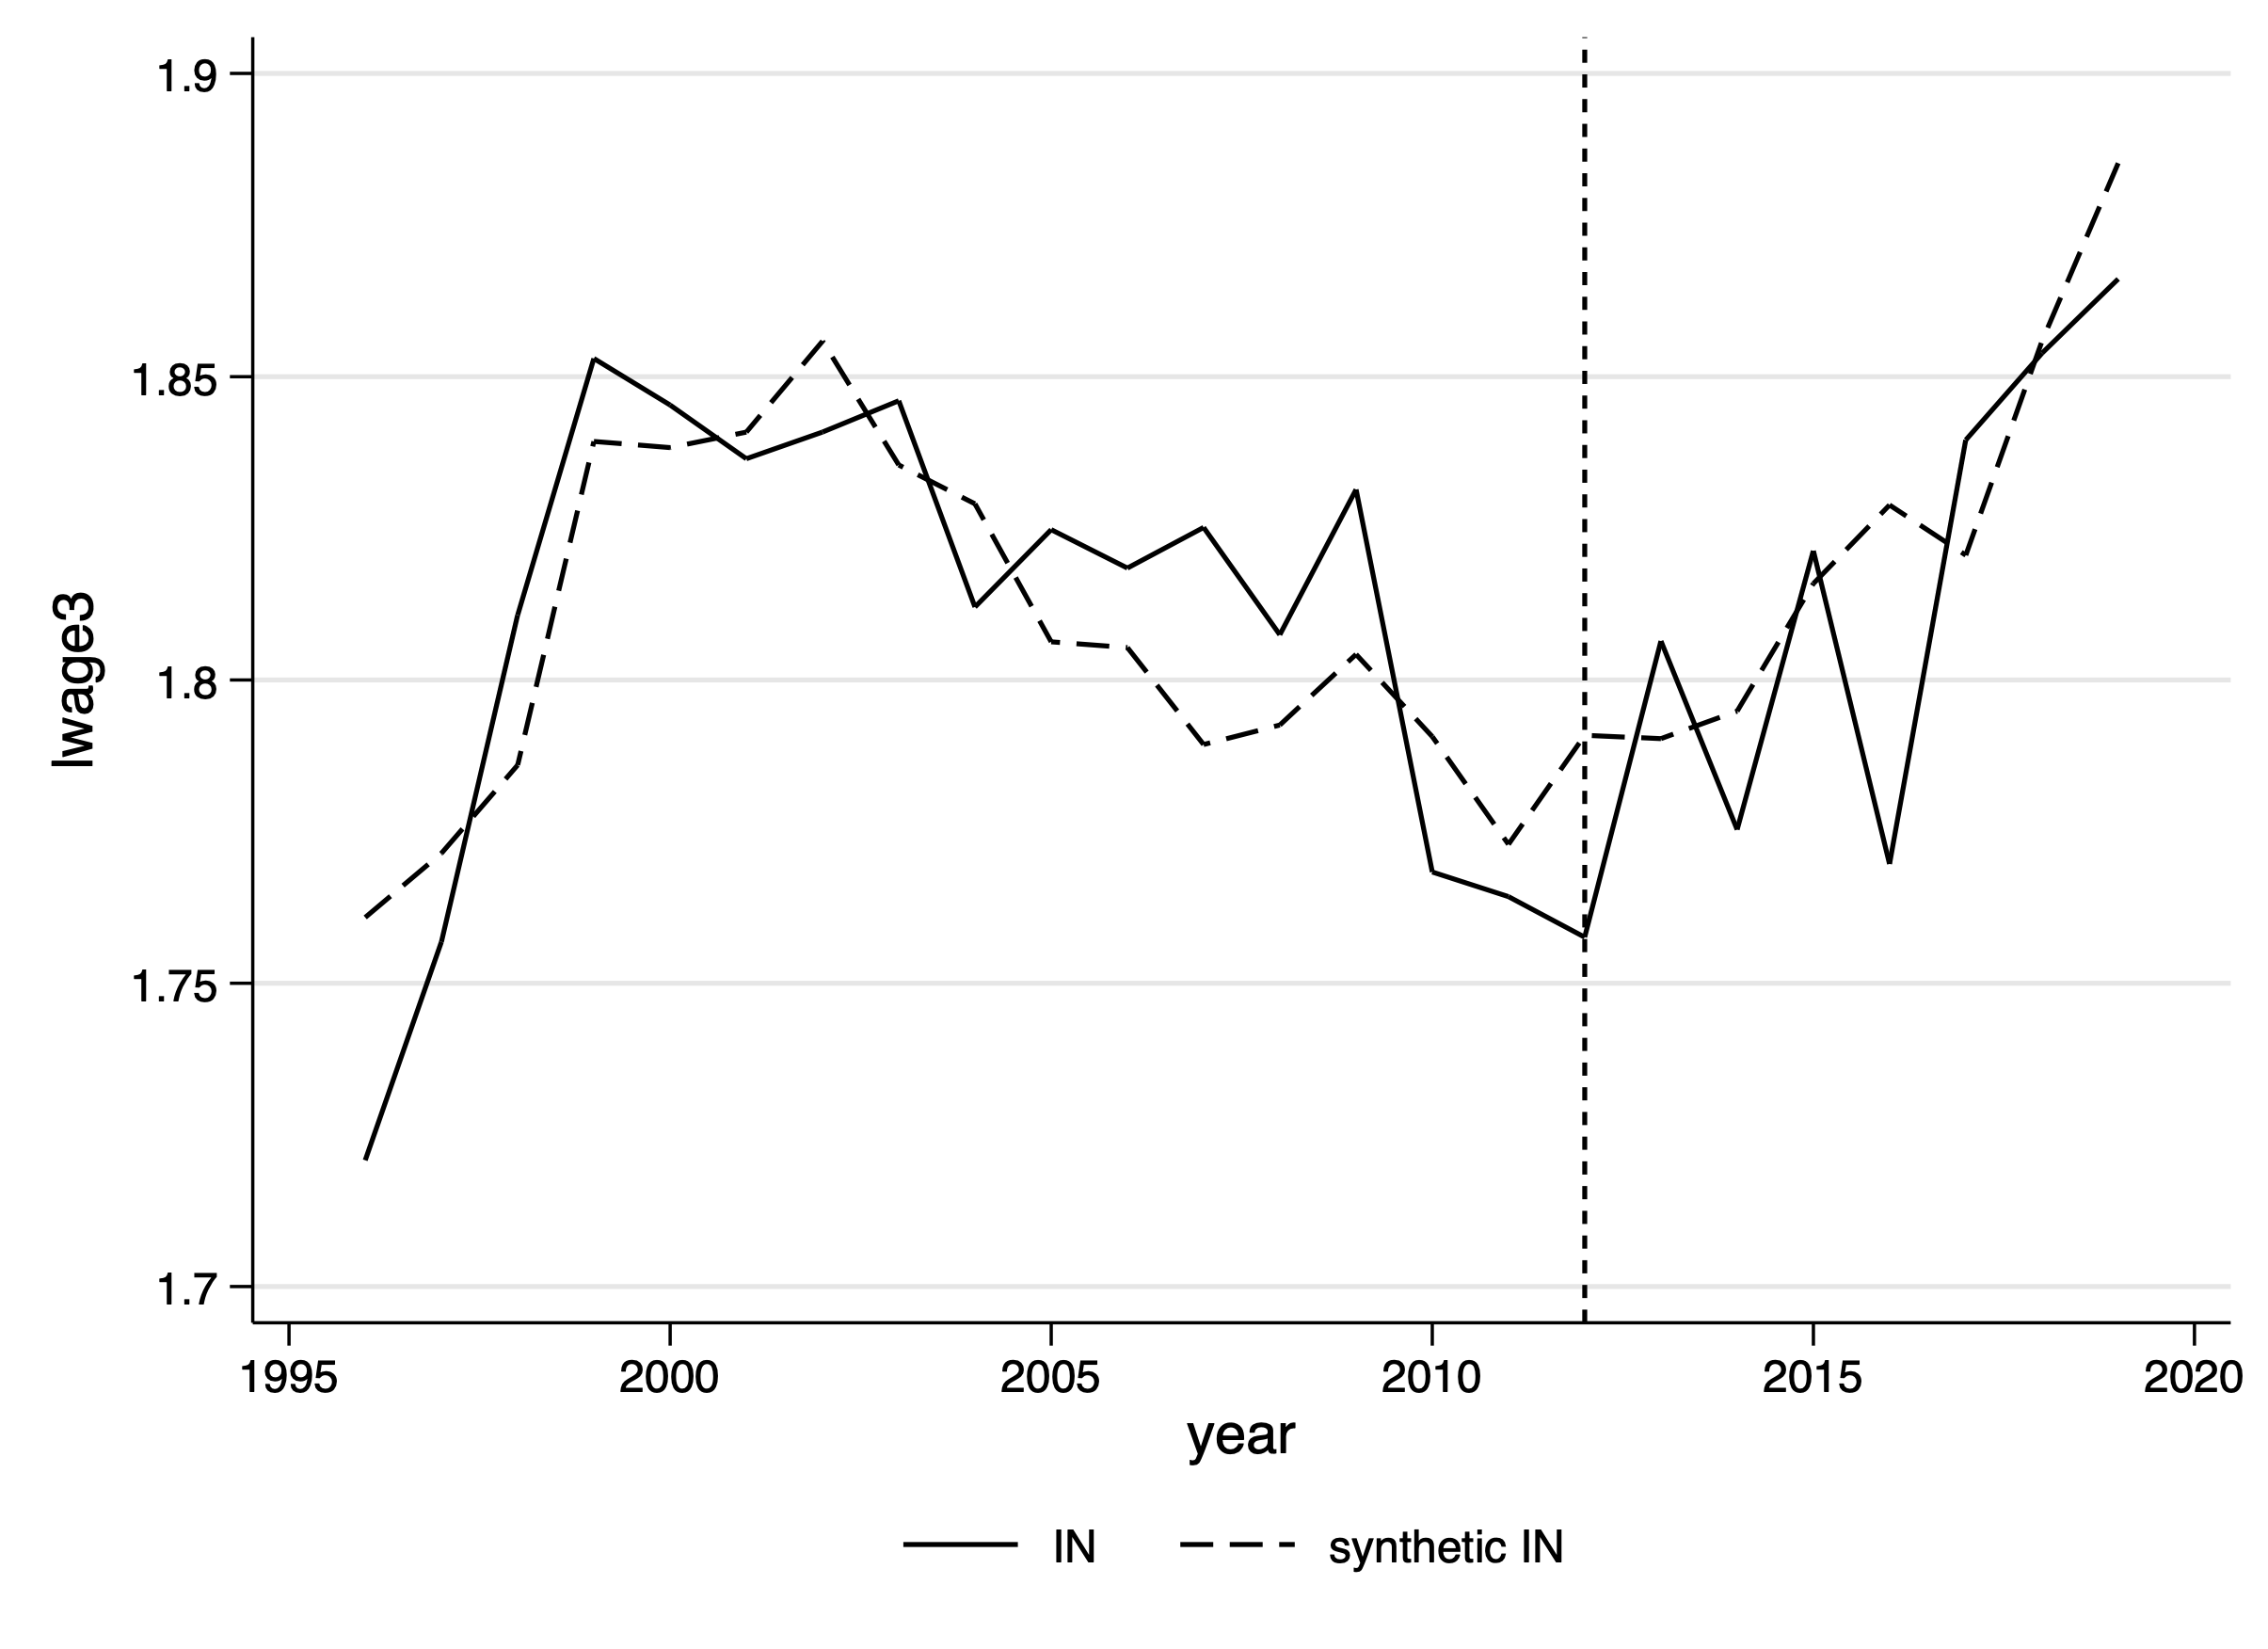
\includegraphics[width = 0.6\textwidth, keepaspectratio]{figures/fin_synth_wm_in.png} & 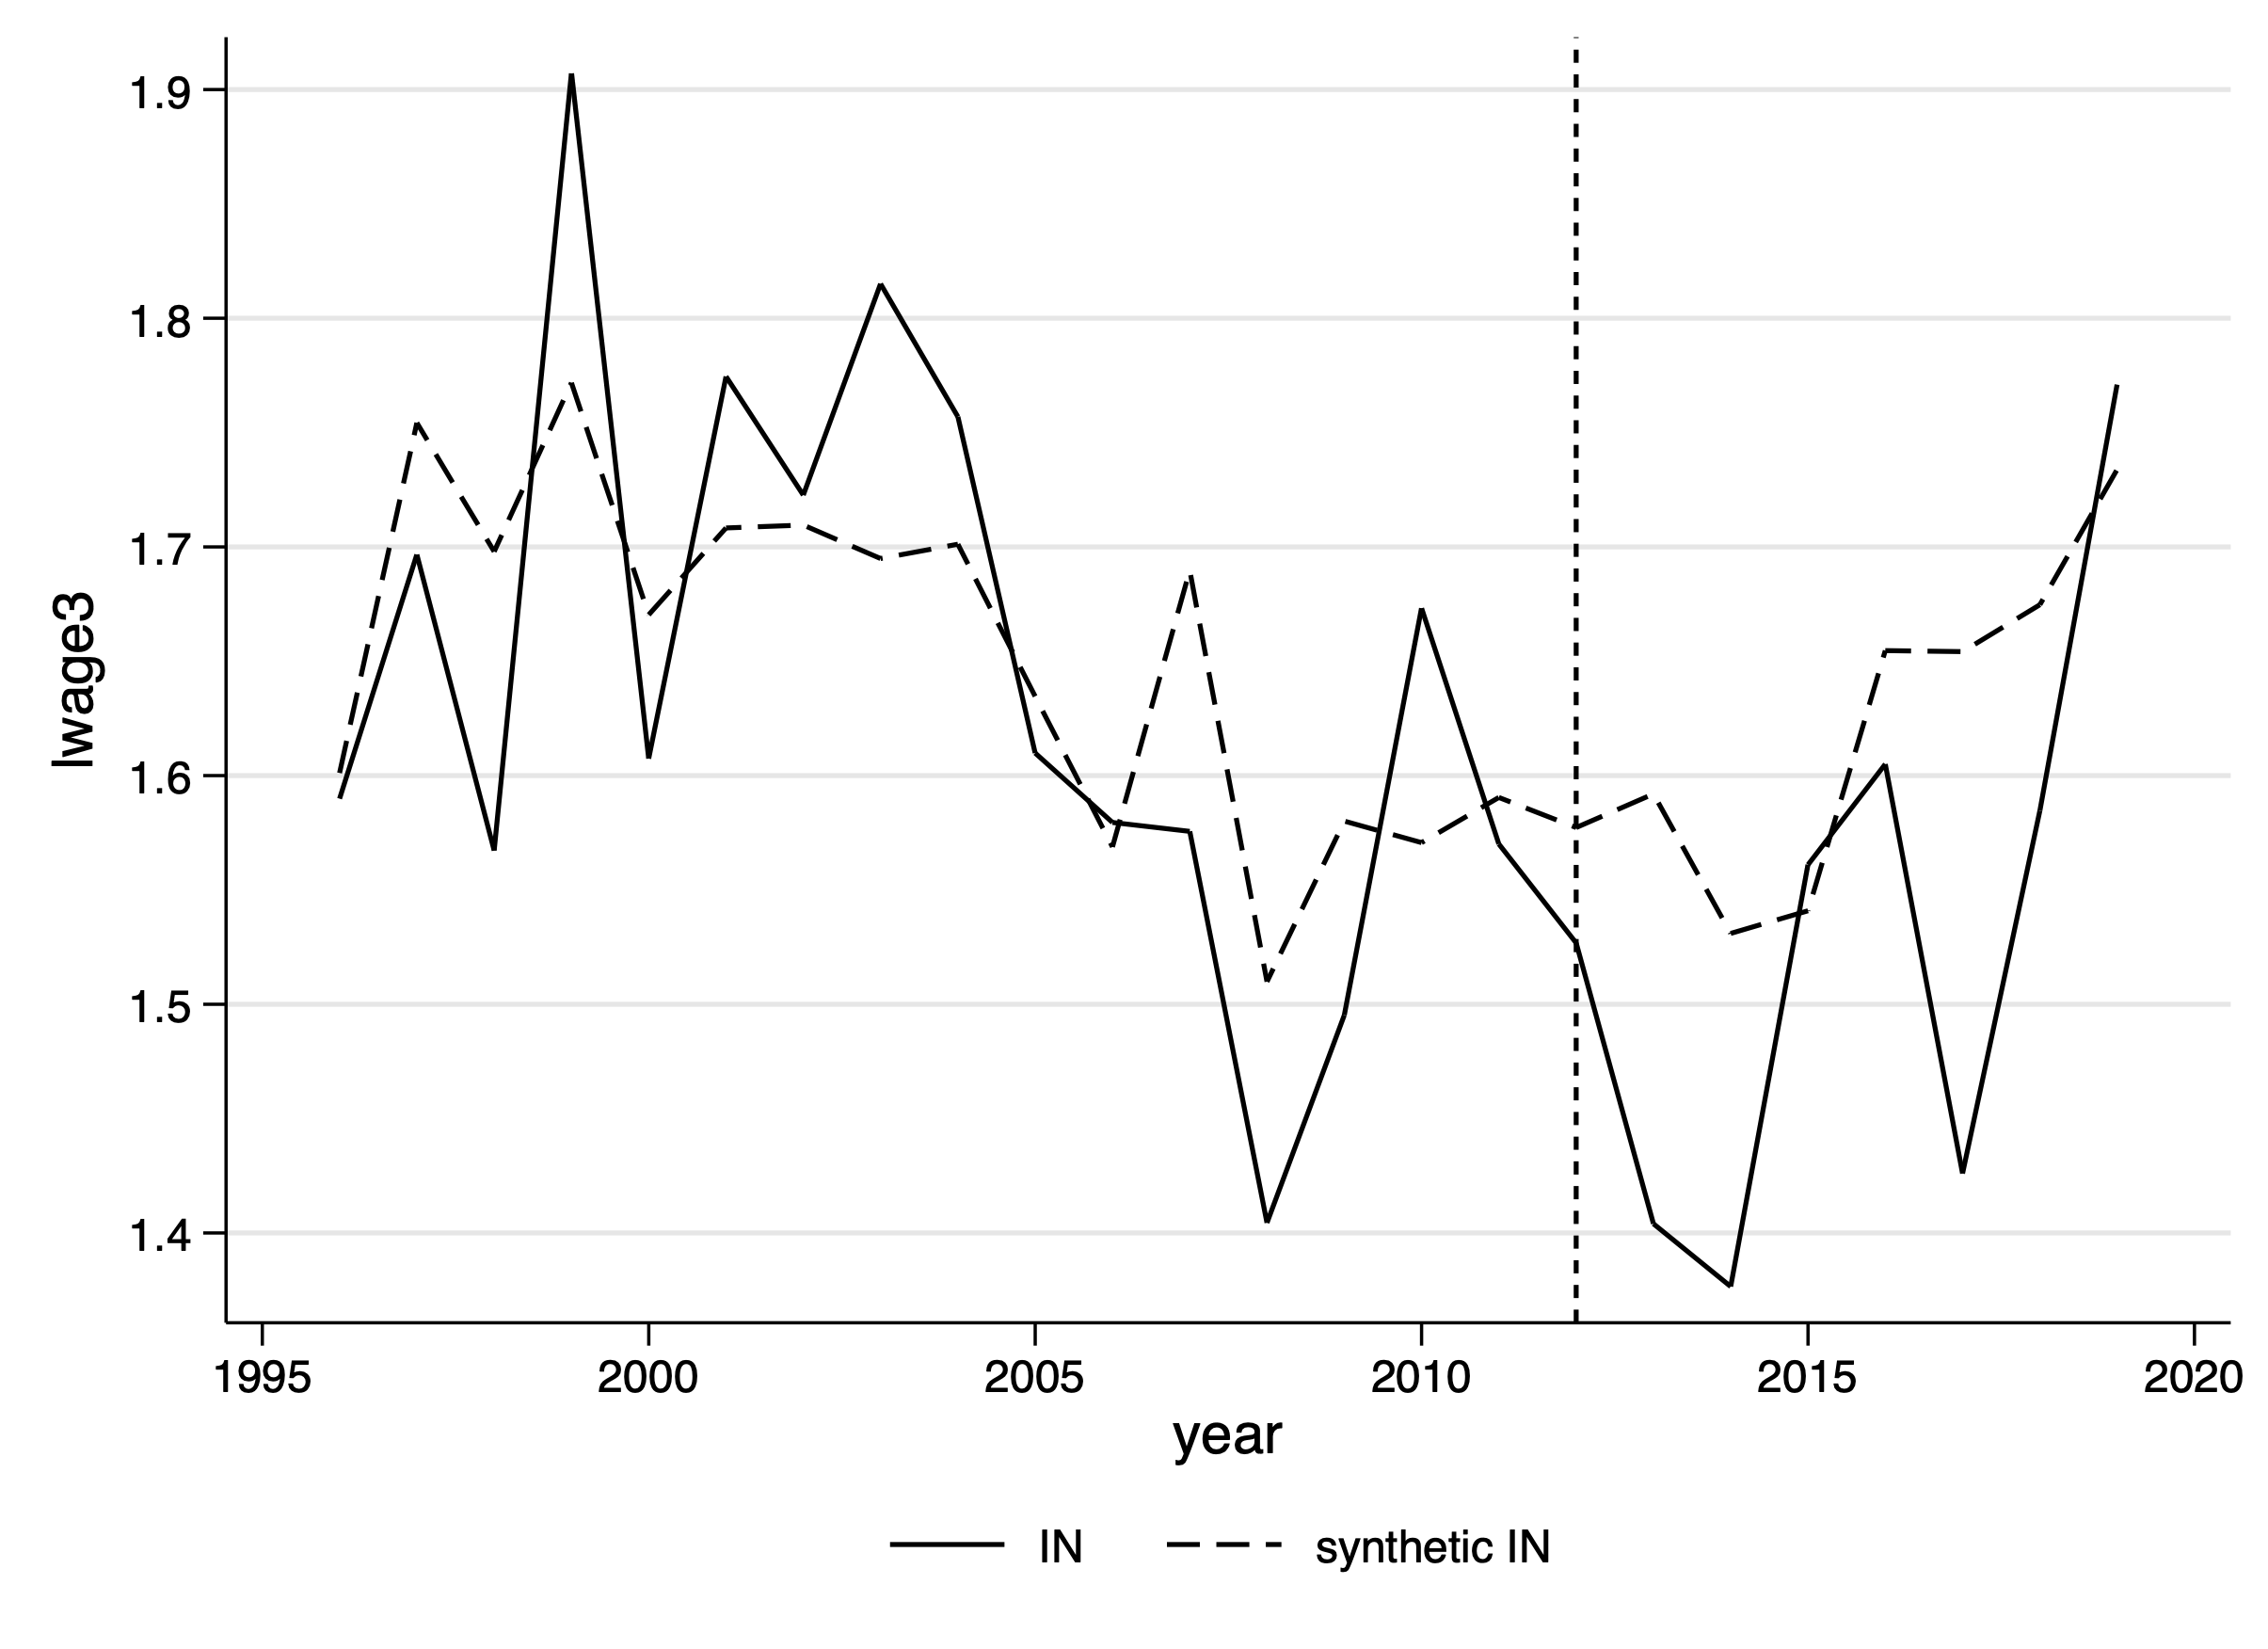
\includegraphics[width = 0.6\textwidth, keepaspectratio]{figures/fin_synth_bm_in.png} \\
          \textbf{White Women} & \textbf{Black Women} \\
          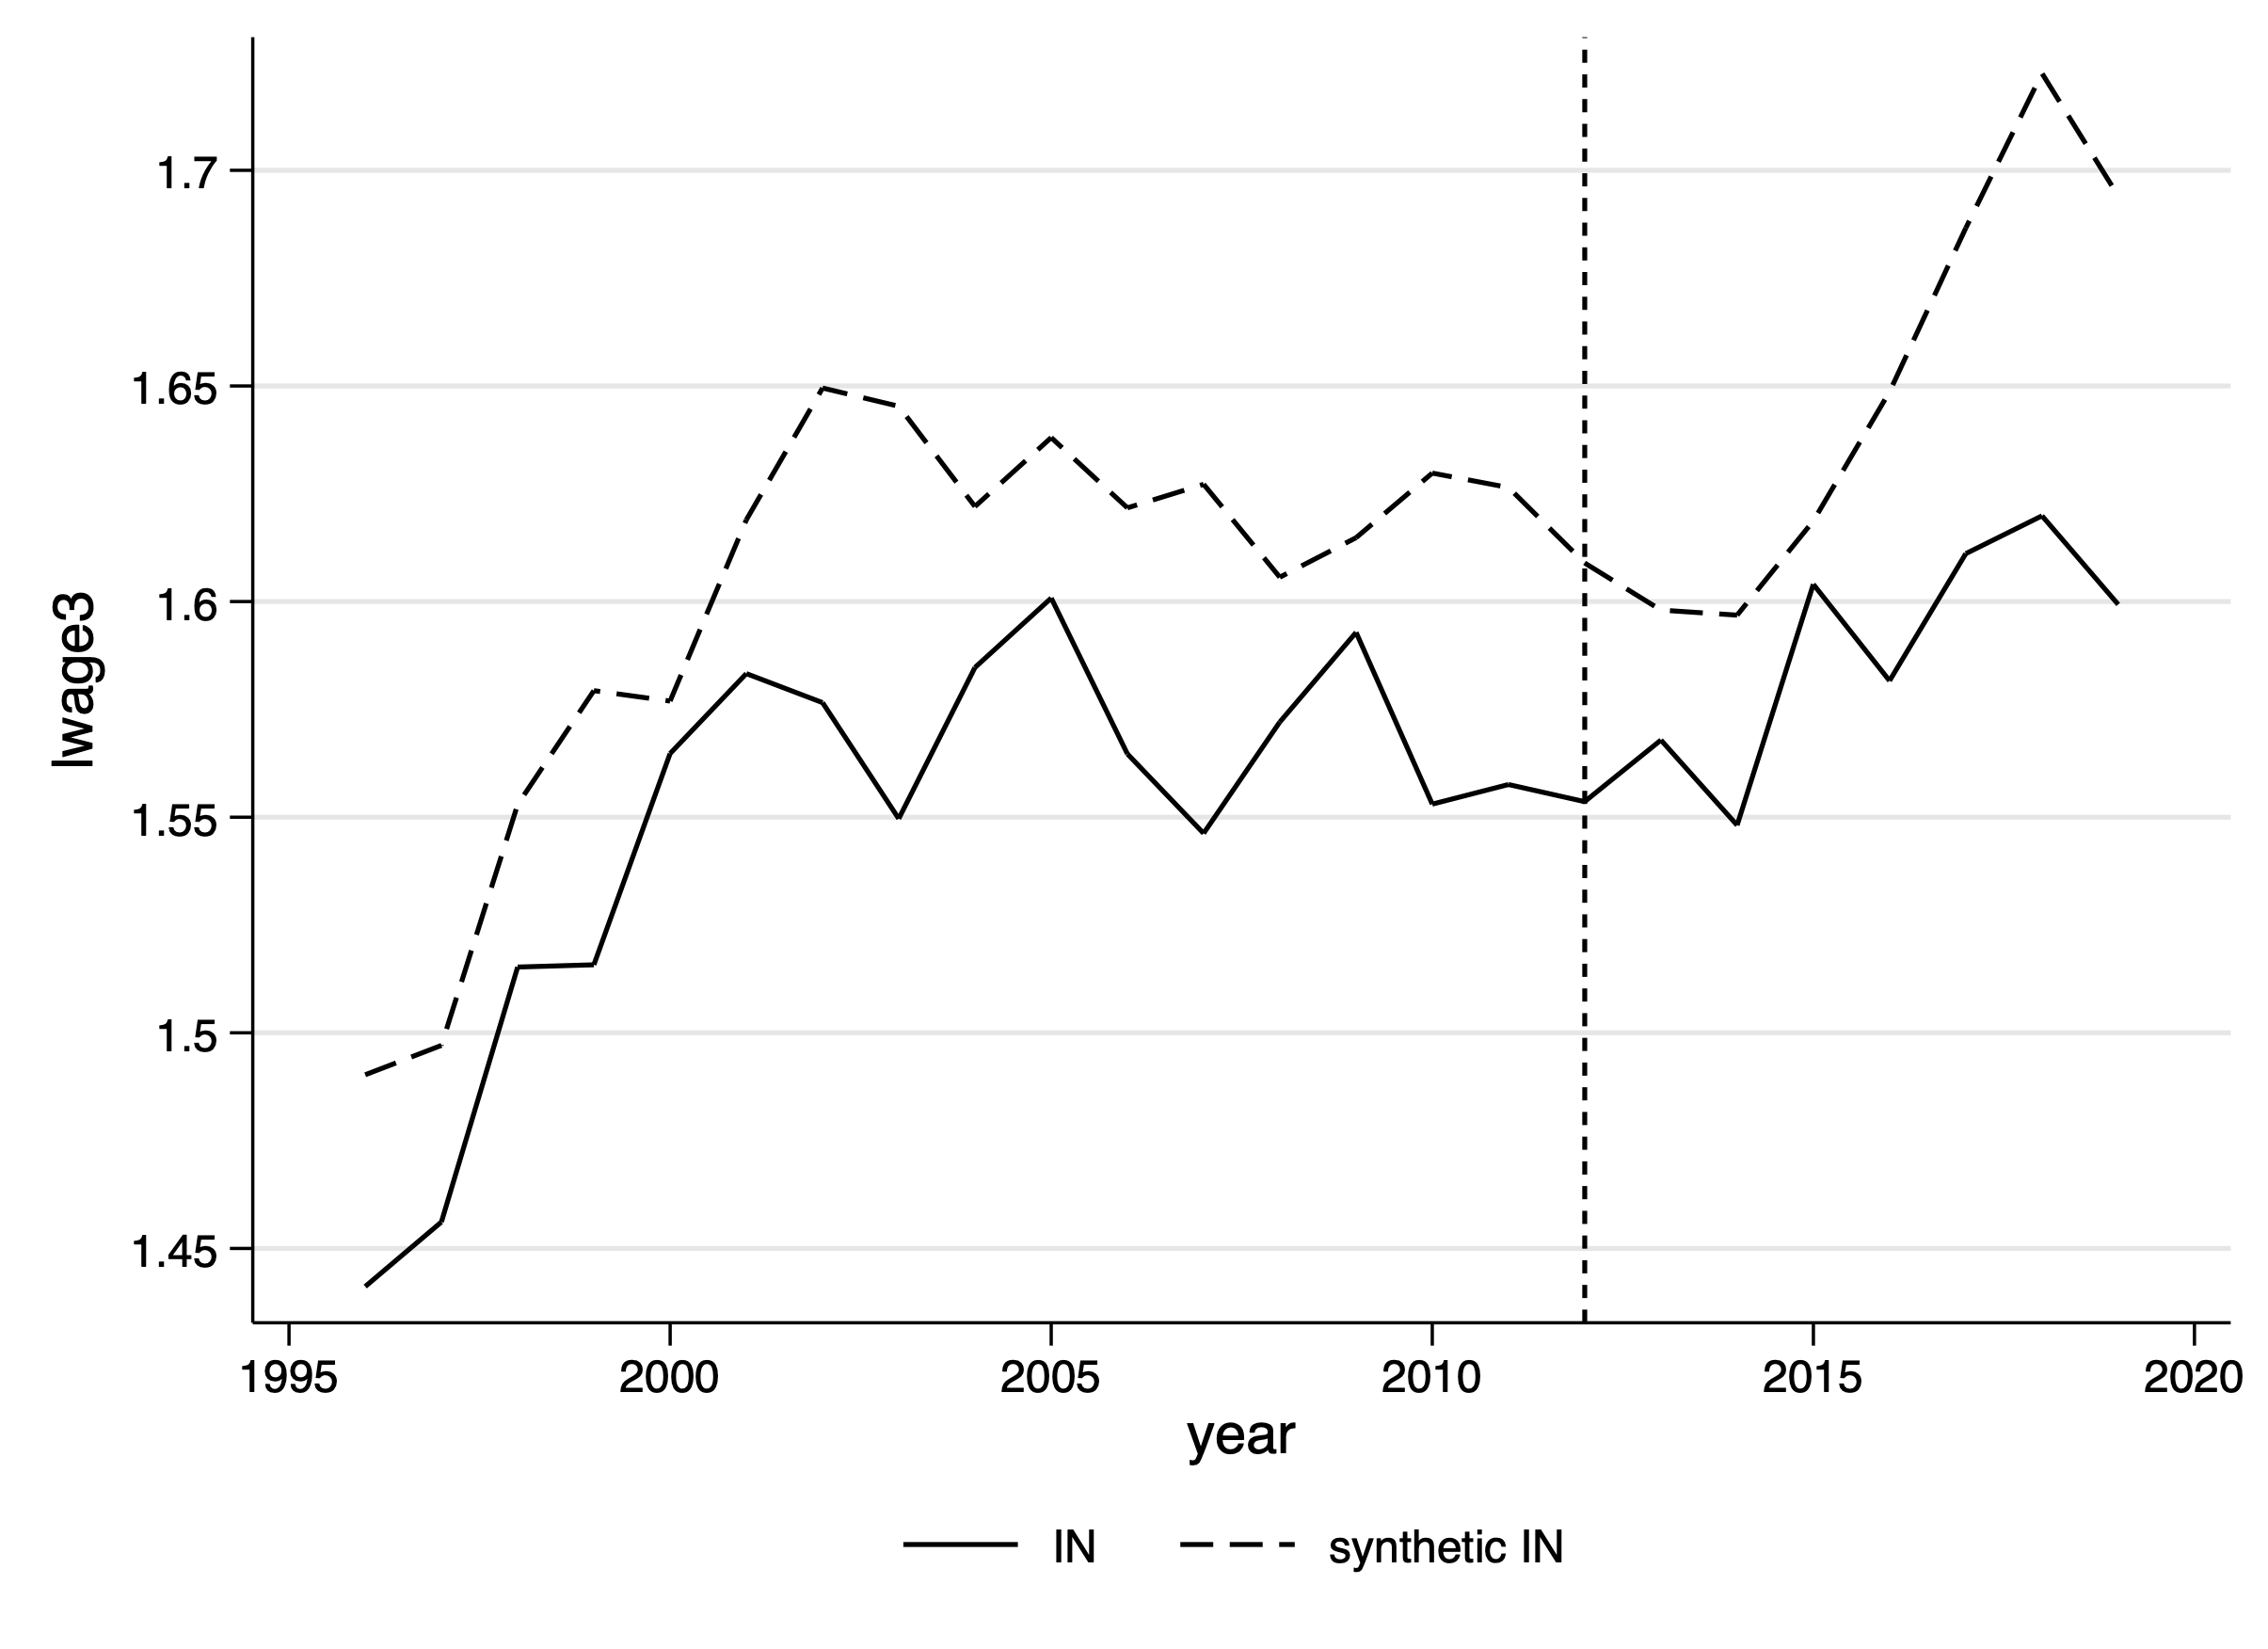
\includegraphics[width = 0.6\textwidth, keepaspectratio]{figures/fin_synth_wf_in.png} & 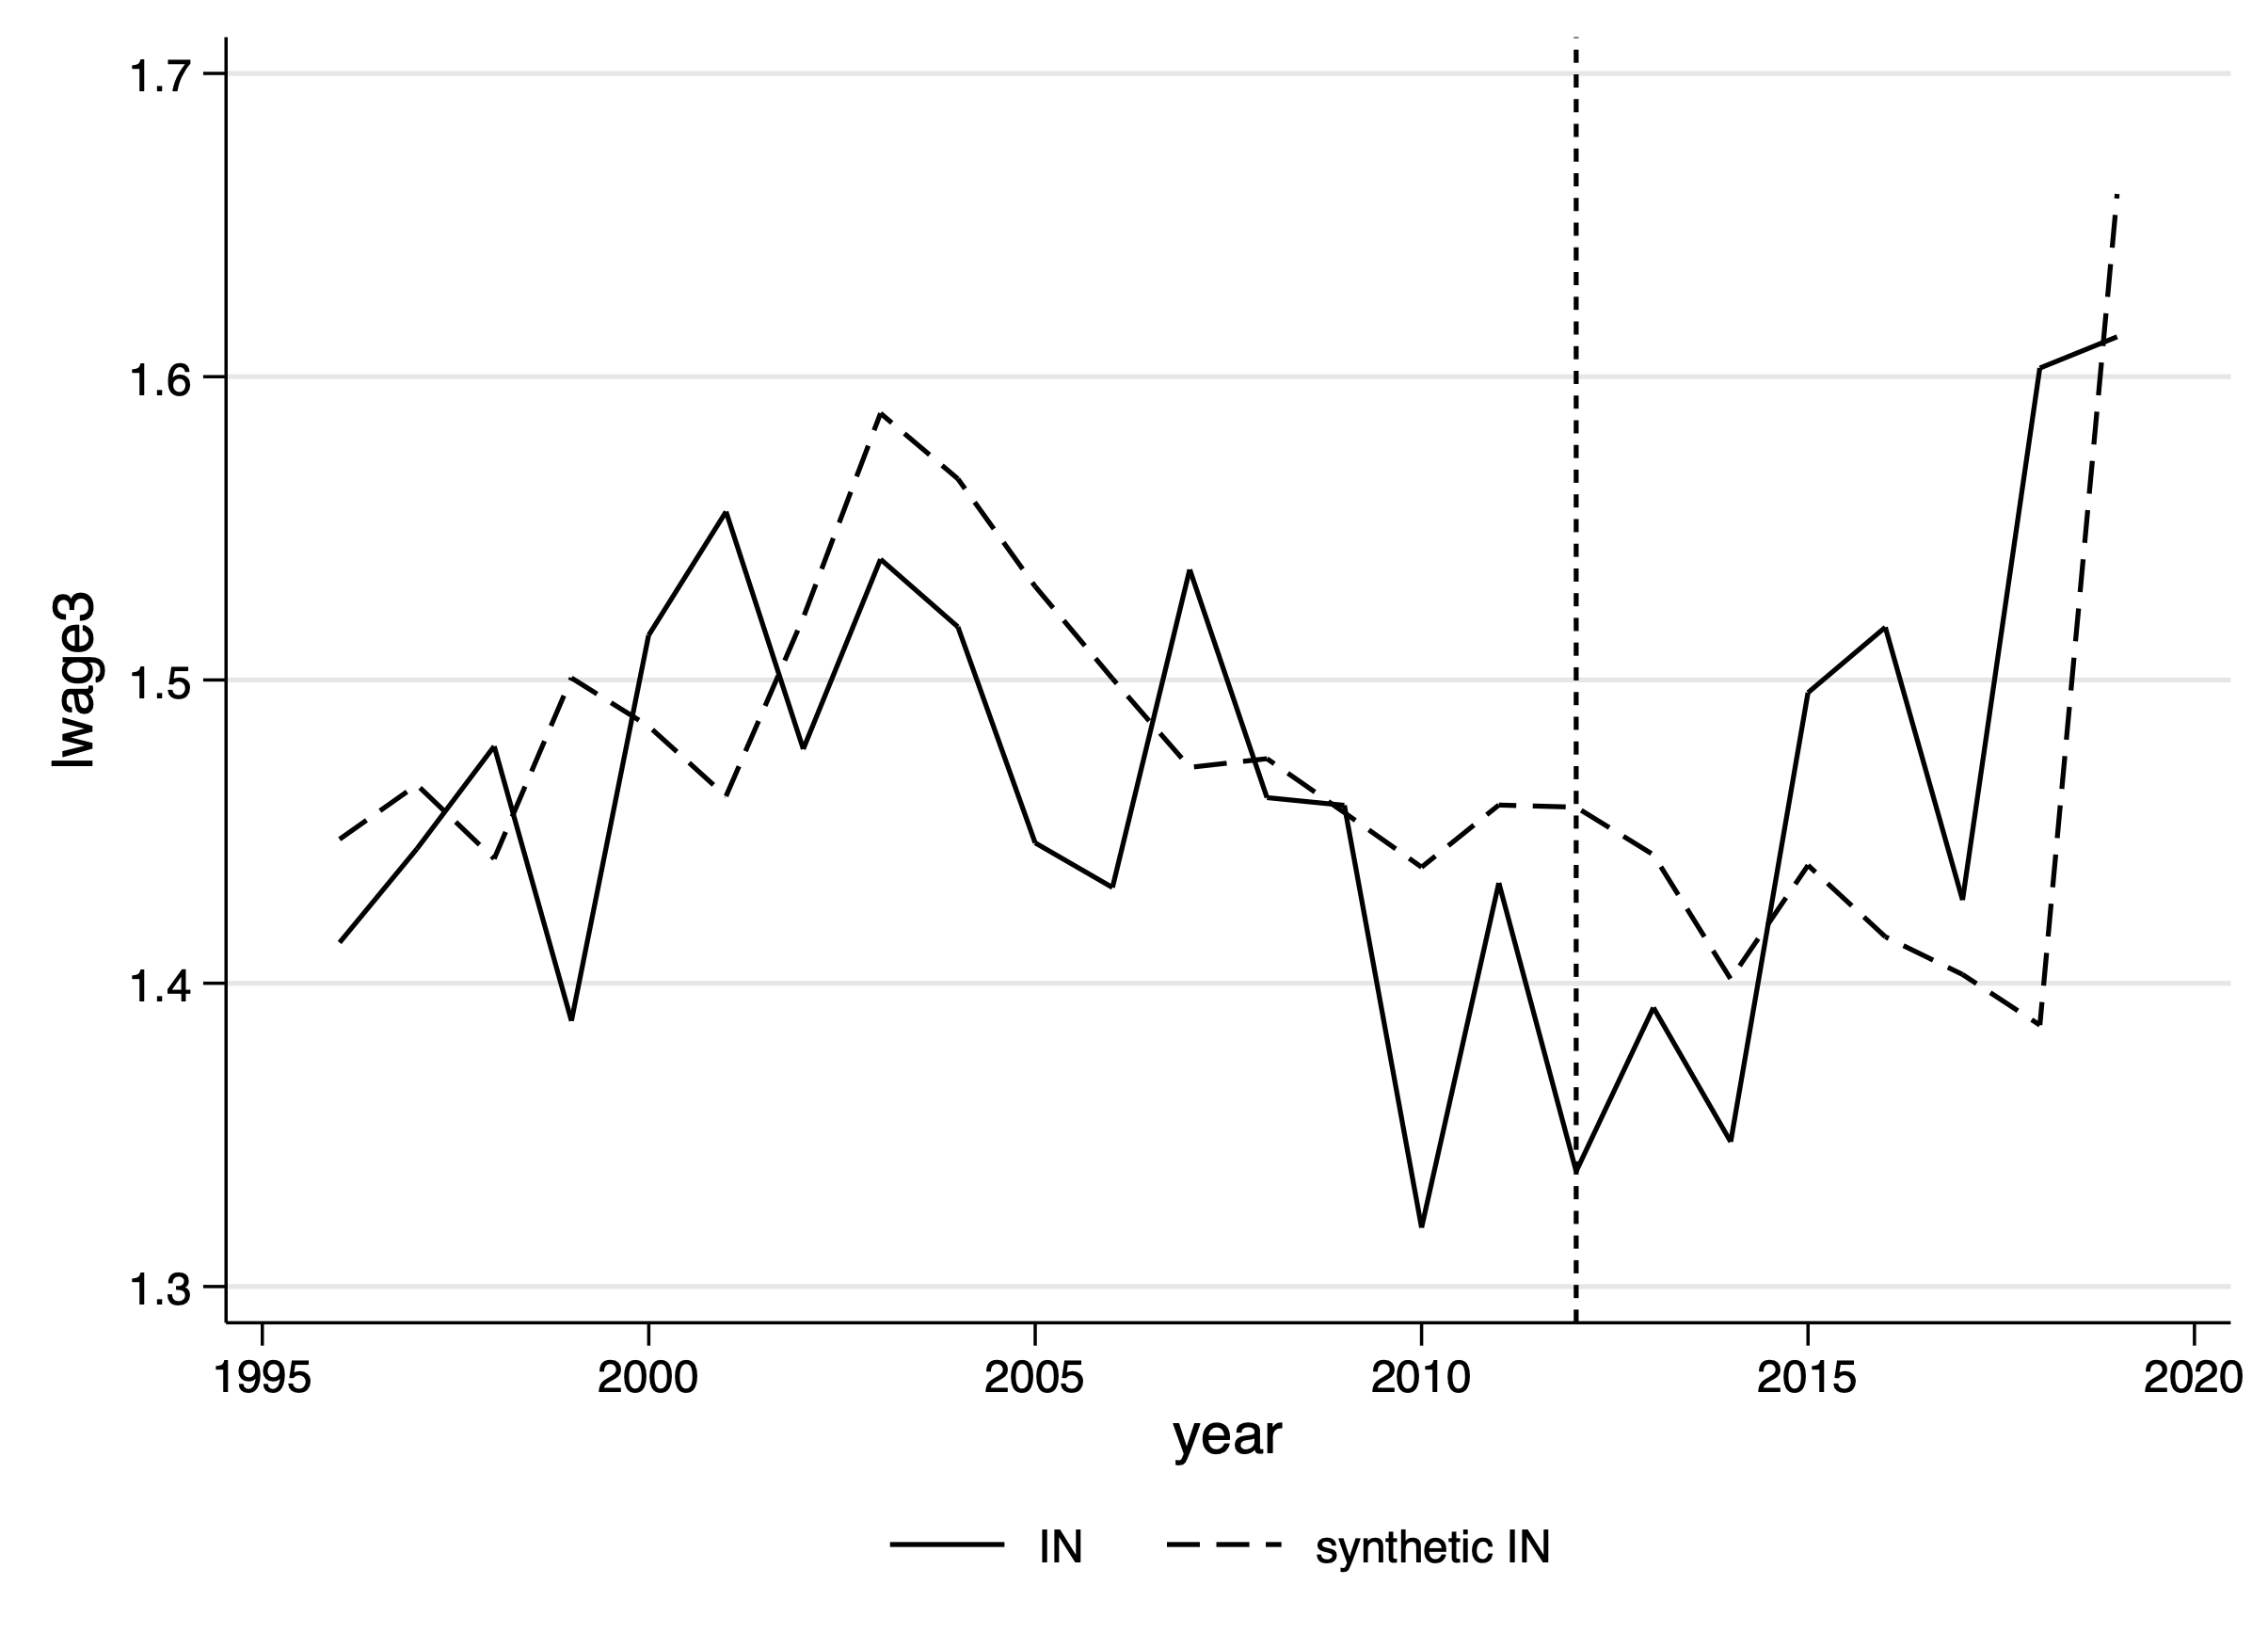
\includegraphics[width = 0.6\textwidth, keepaspectratio]{figures/fin_synth_bf_in.png}
    \end{tabular}
\end{table}
% \footnotesize{Sample include years 1983-2019 excluding 1994 and 1995.}
\end{landscape}

\pagebreak
\begin{landscape}
\begin{table}[ht!]
    \centering
    \captionof{figure}{Synthetic Control Method - Michigan (2013)}\label{fig:synth_mi}
    \begin{tabular}{c c}
          \textbf{White Men} & \textbf{Black Men} \\    
          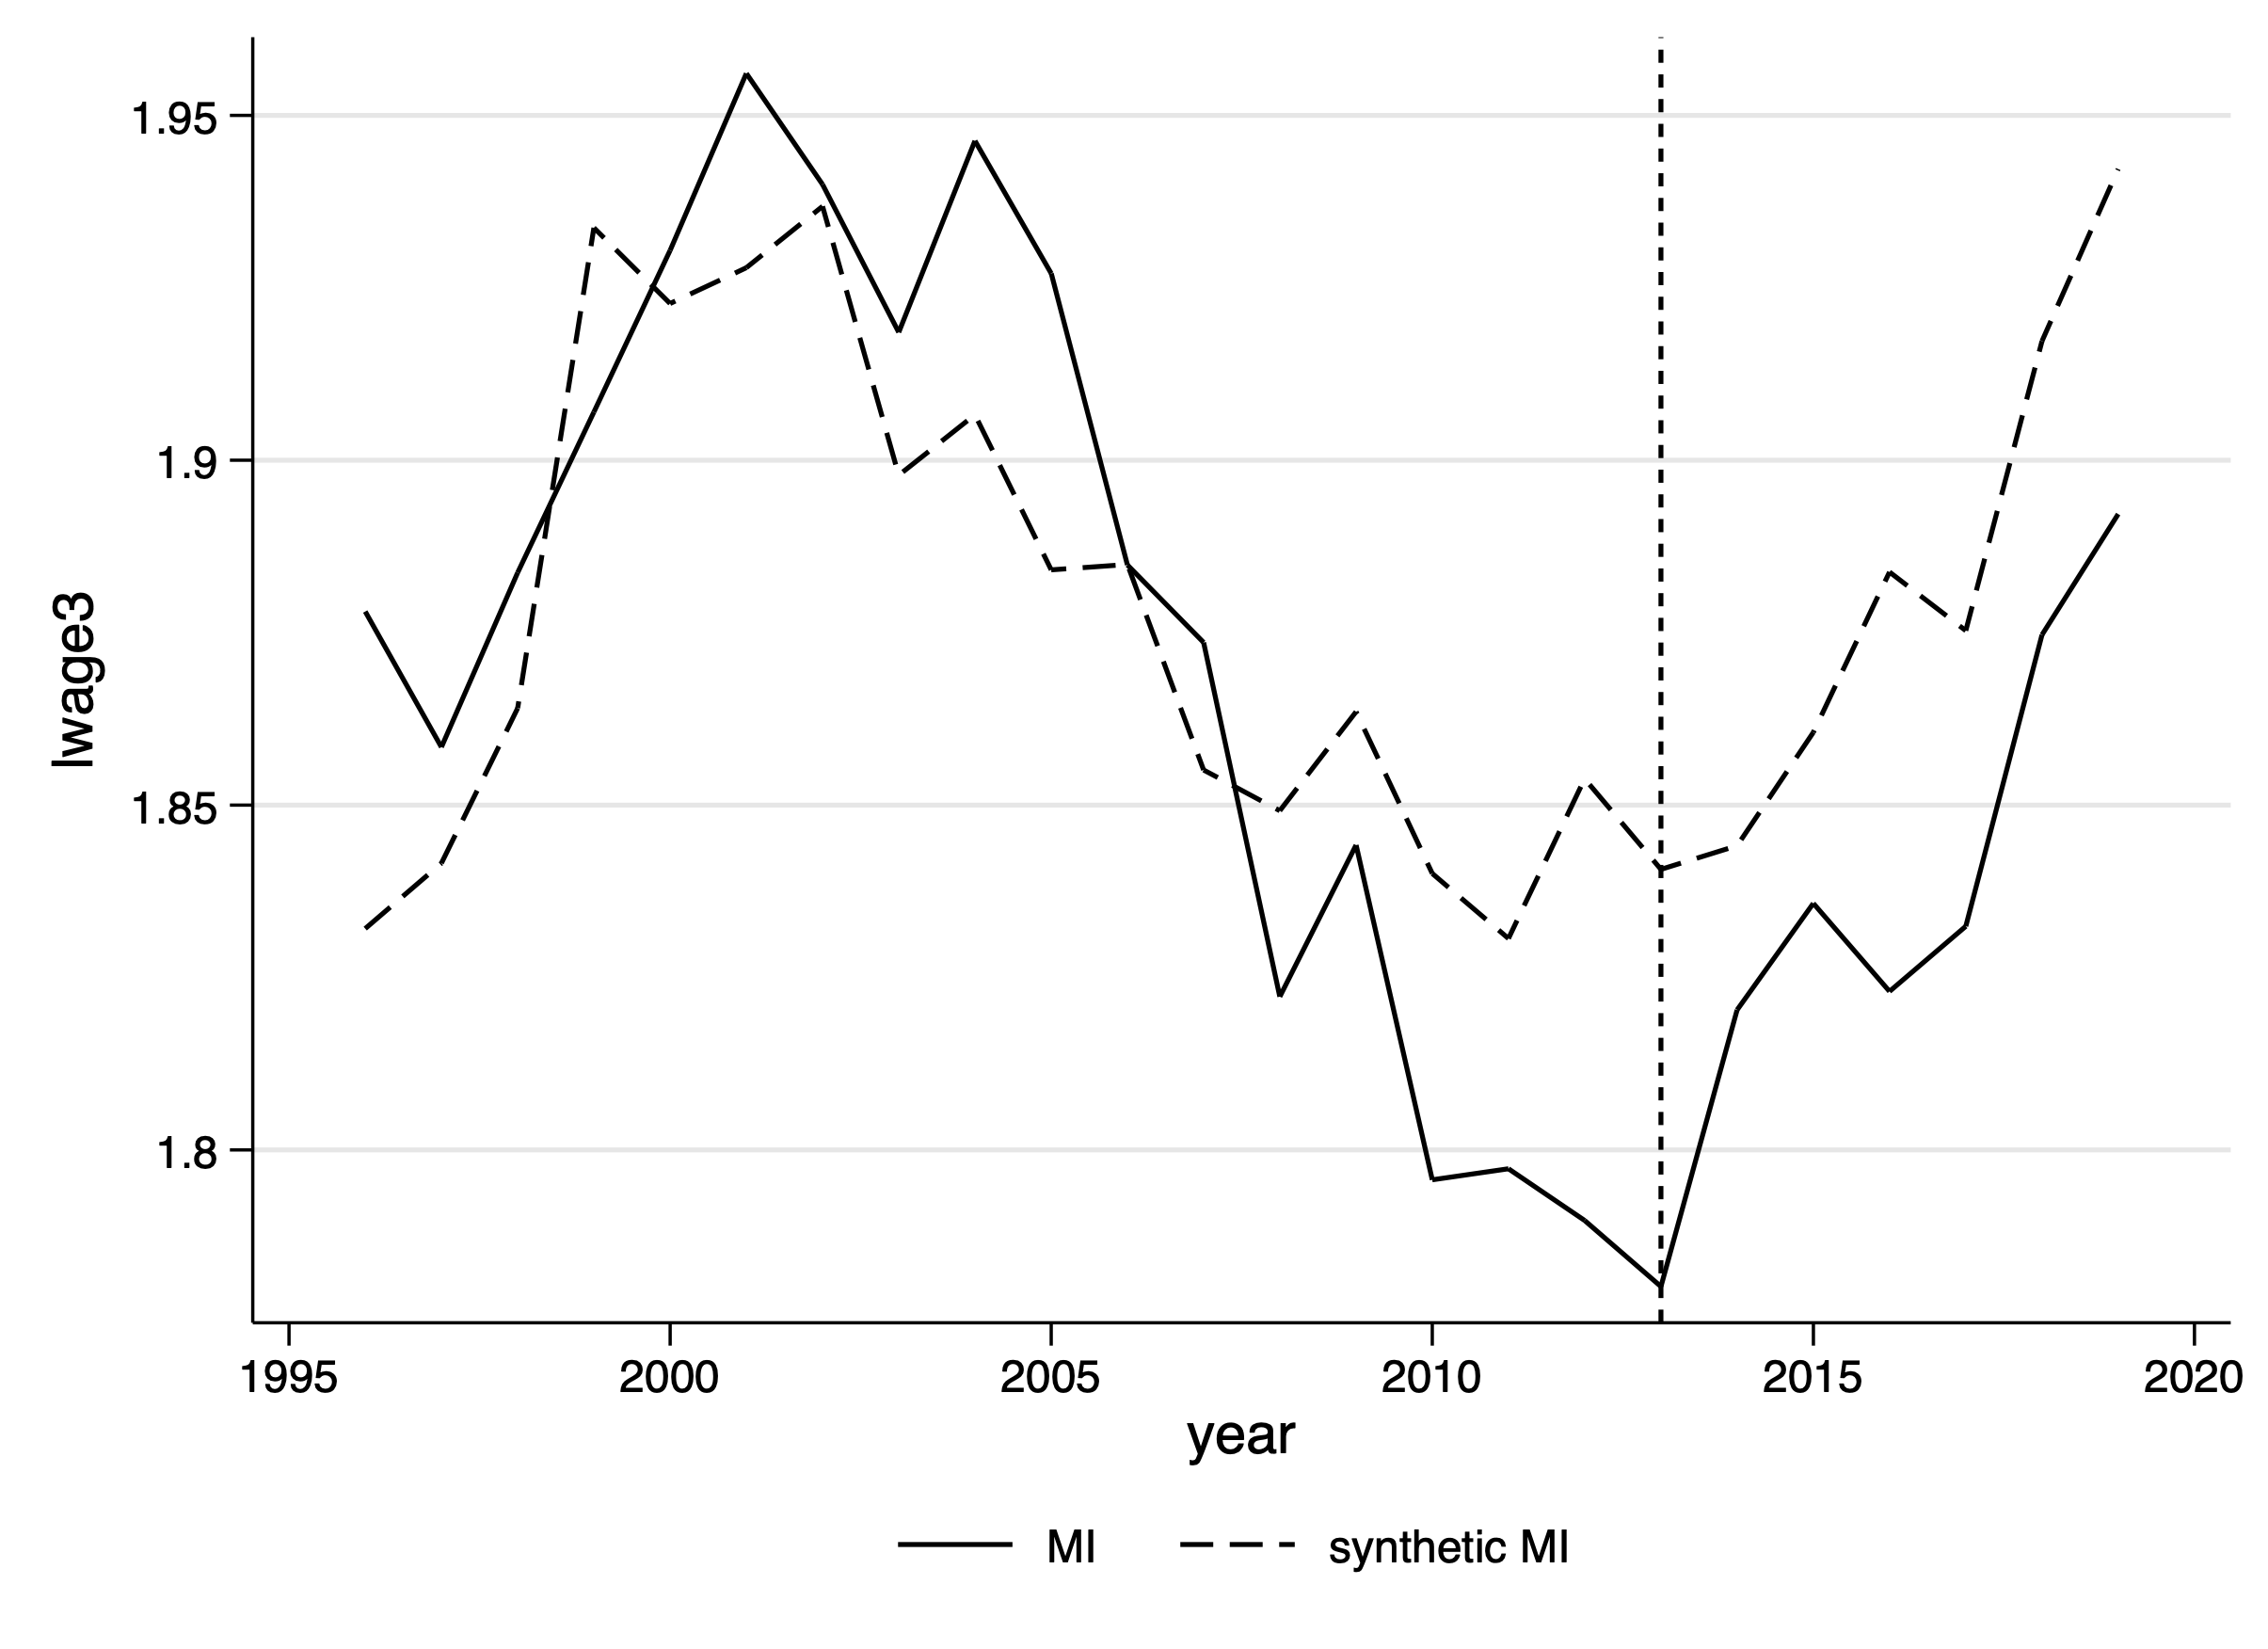
\includegraphics[width = 0.6\textwidth, keepaspectratio]{figures/fin_synth_wm_mi.png} & 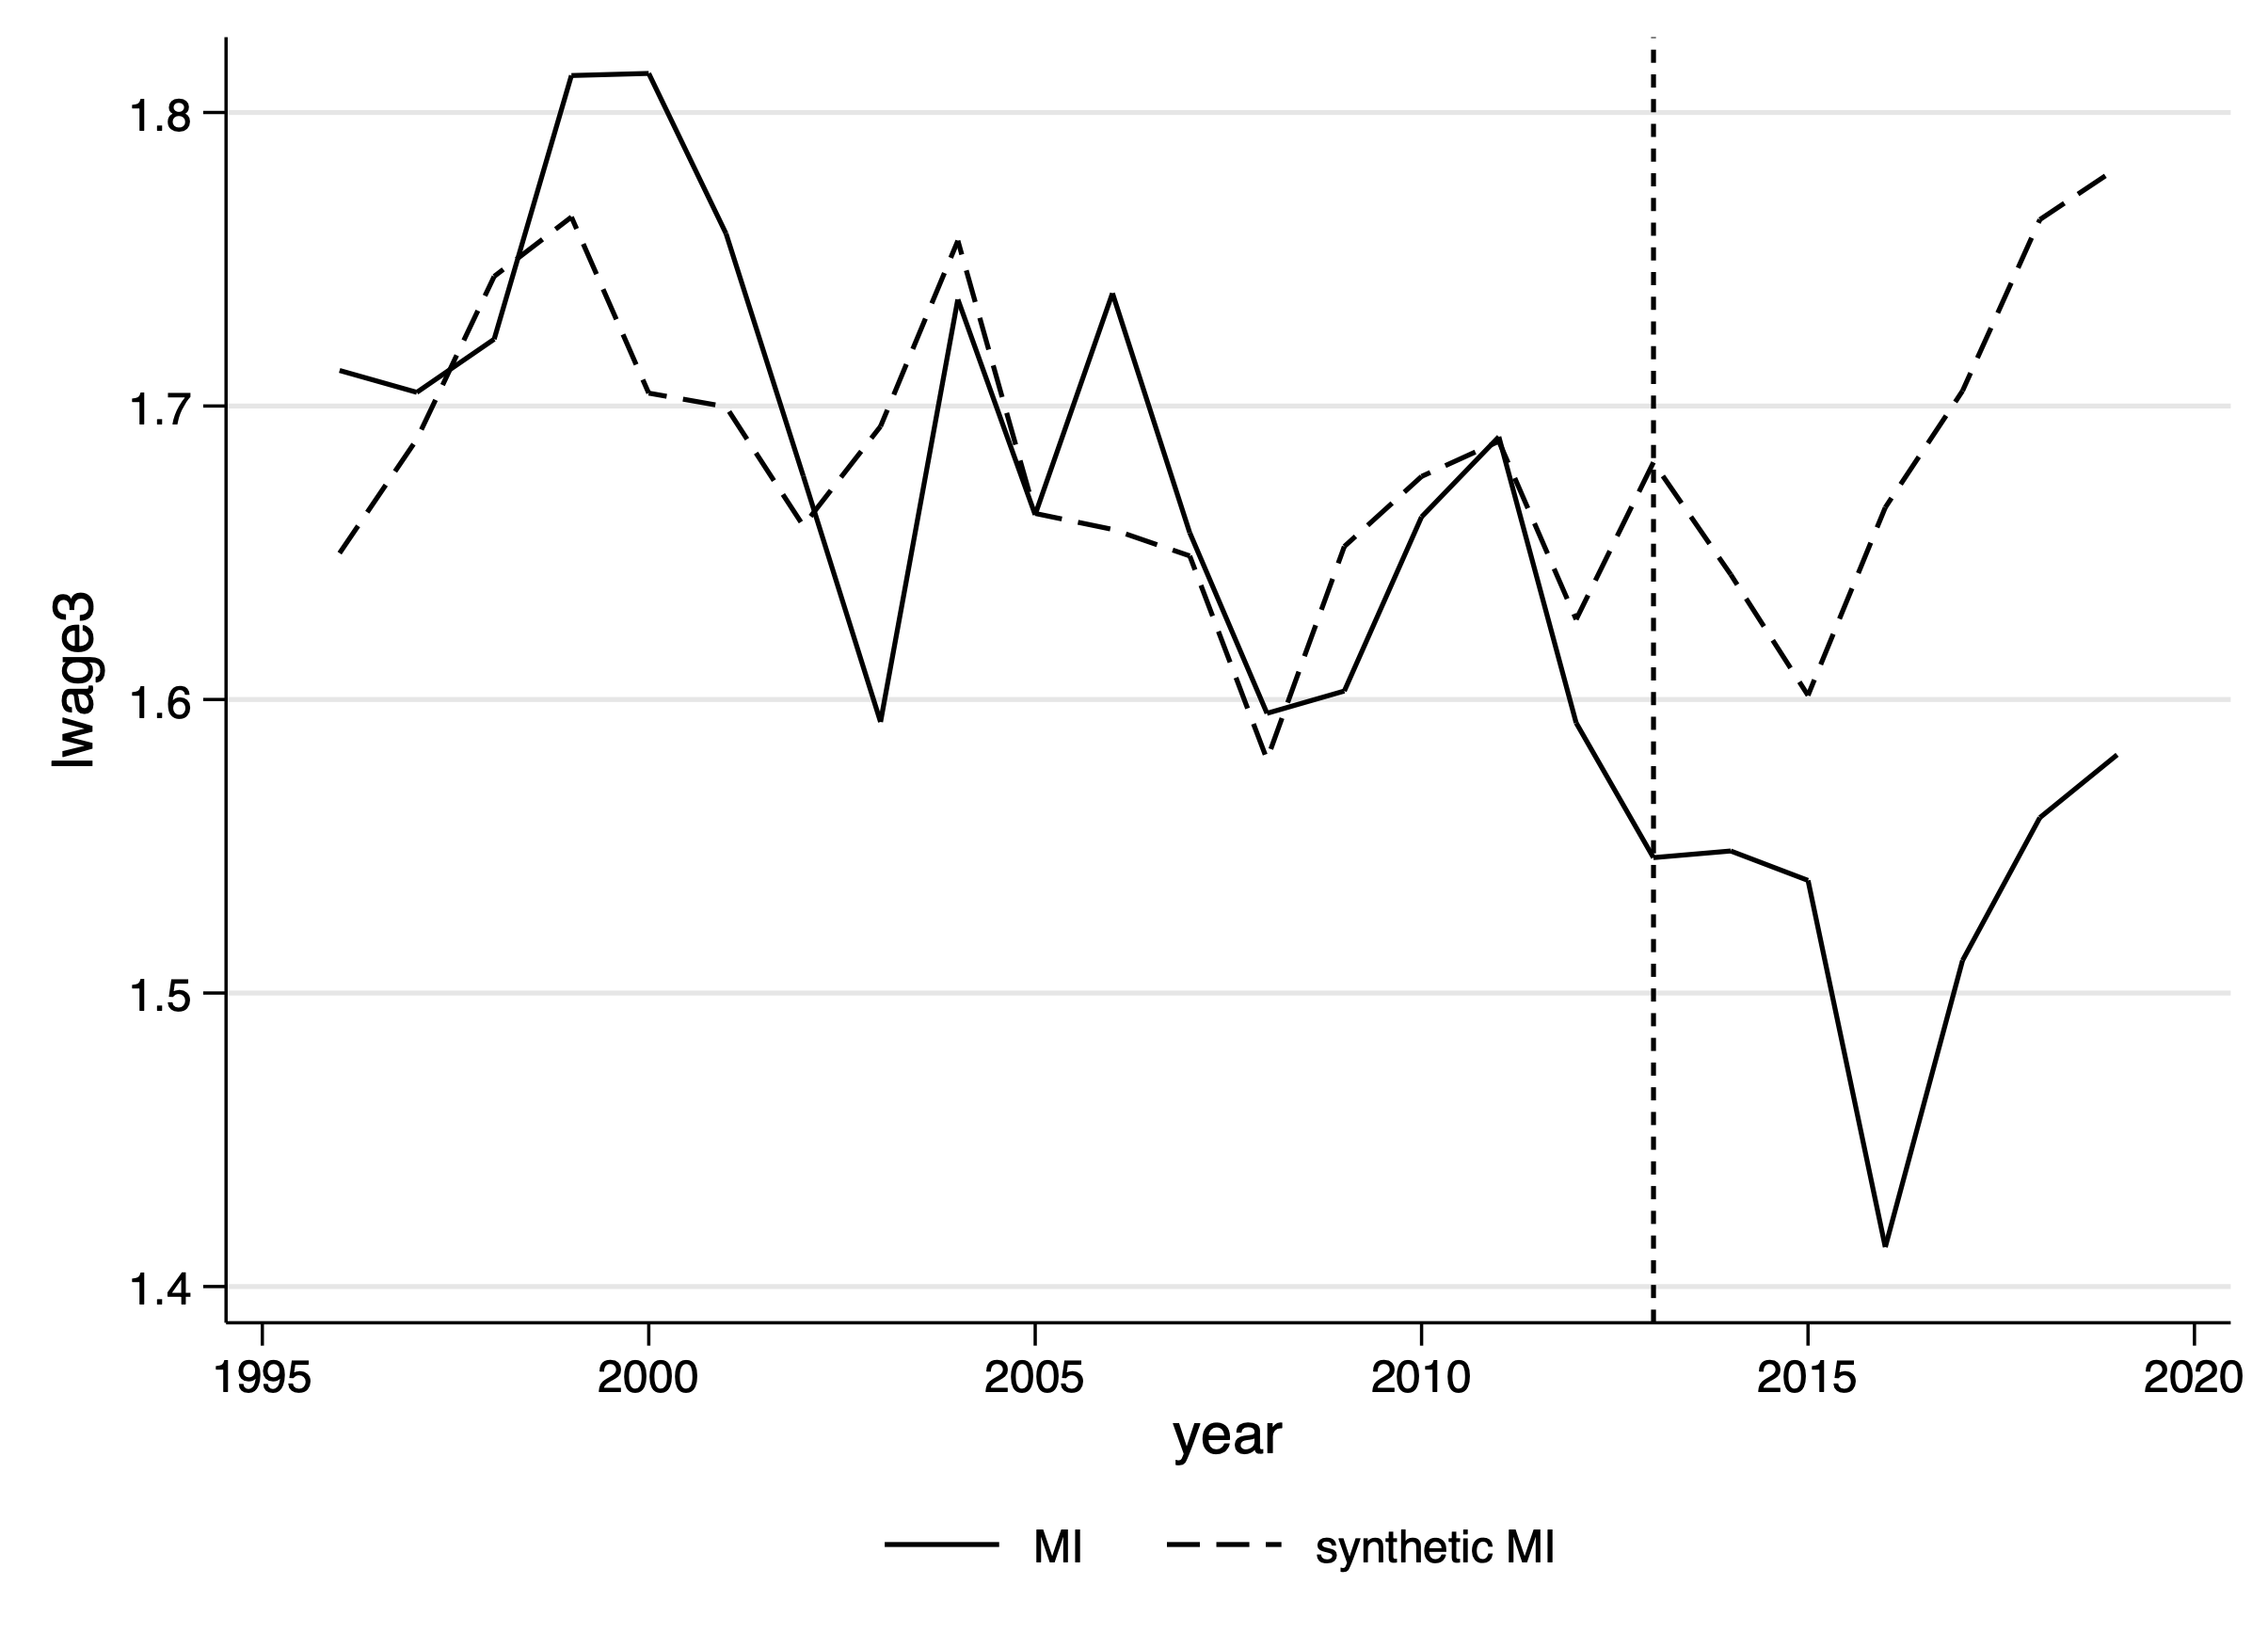
\includegraphics[width = 0.6\textwidth, keepaspectratio]{figures/fin_synth_bm_mi.png} \\
          \textbf{White Women} & \textbf{Black Women} \\
          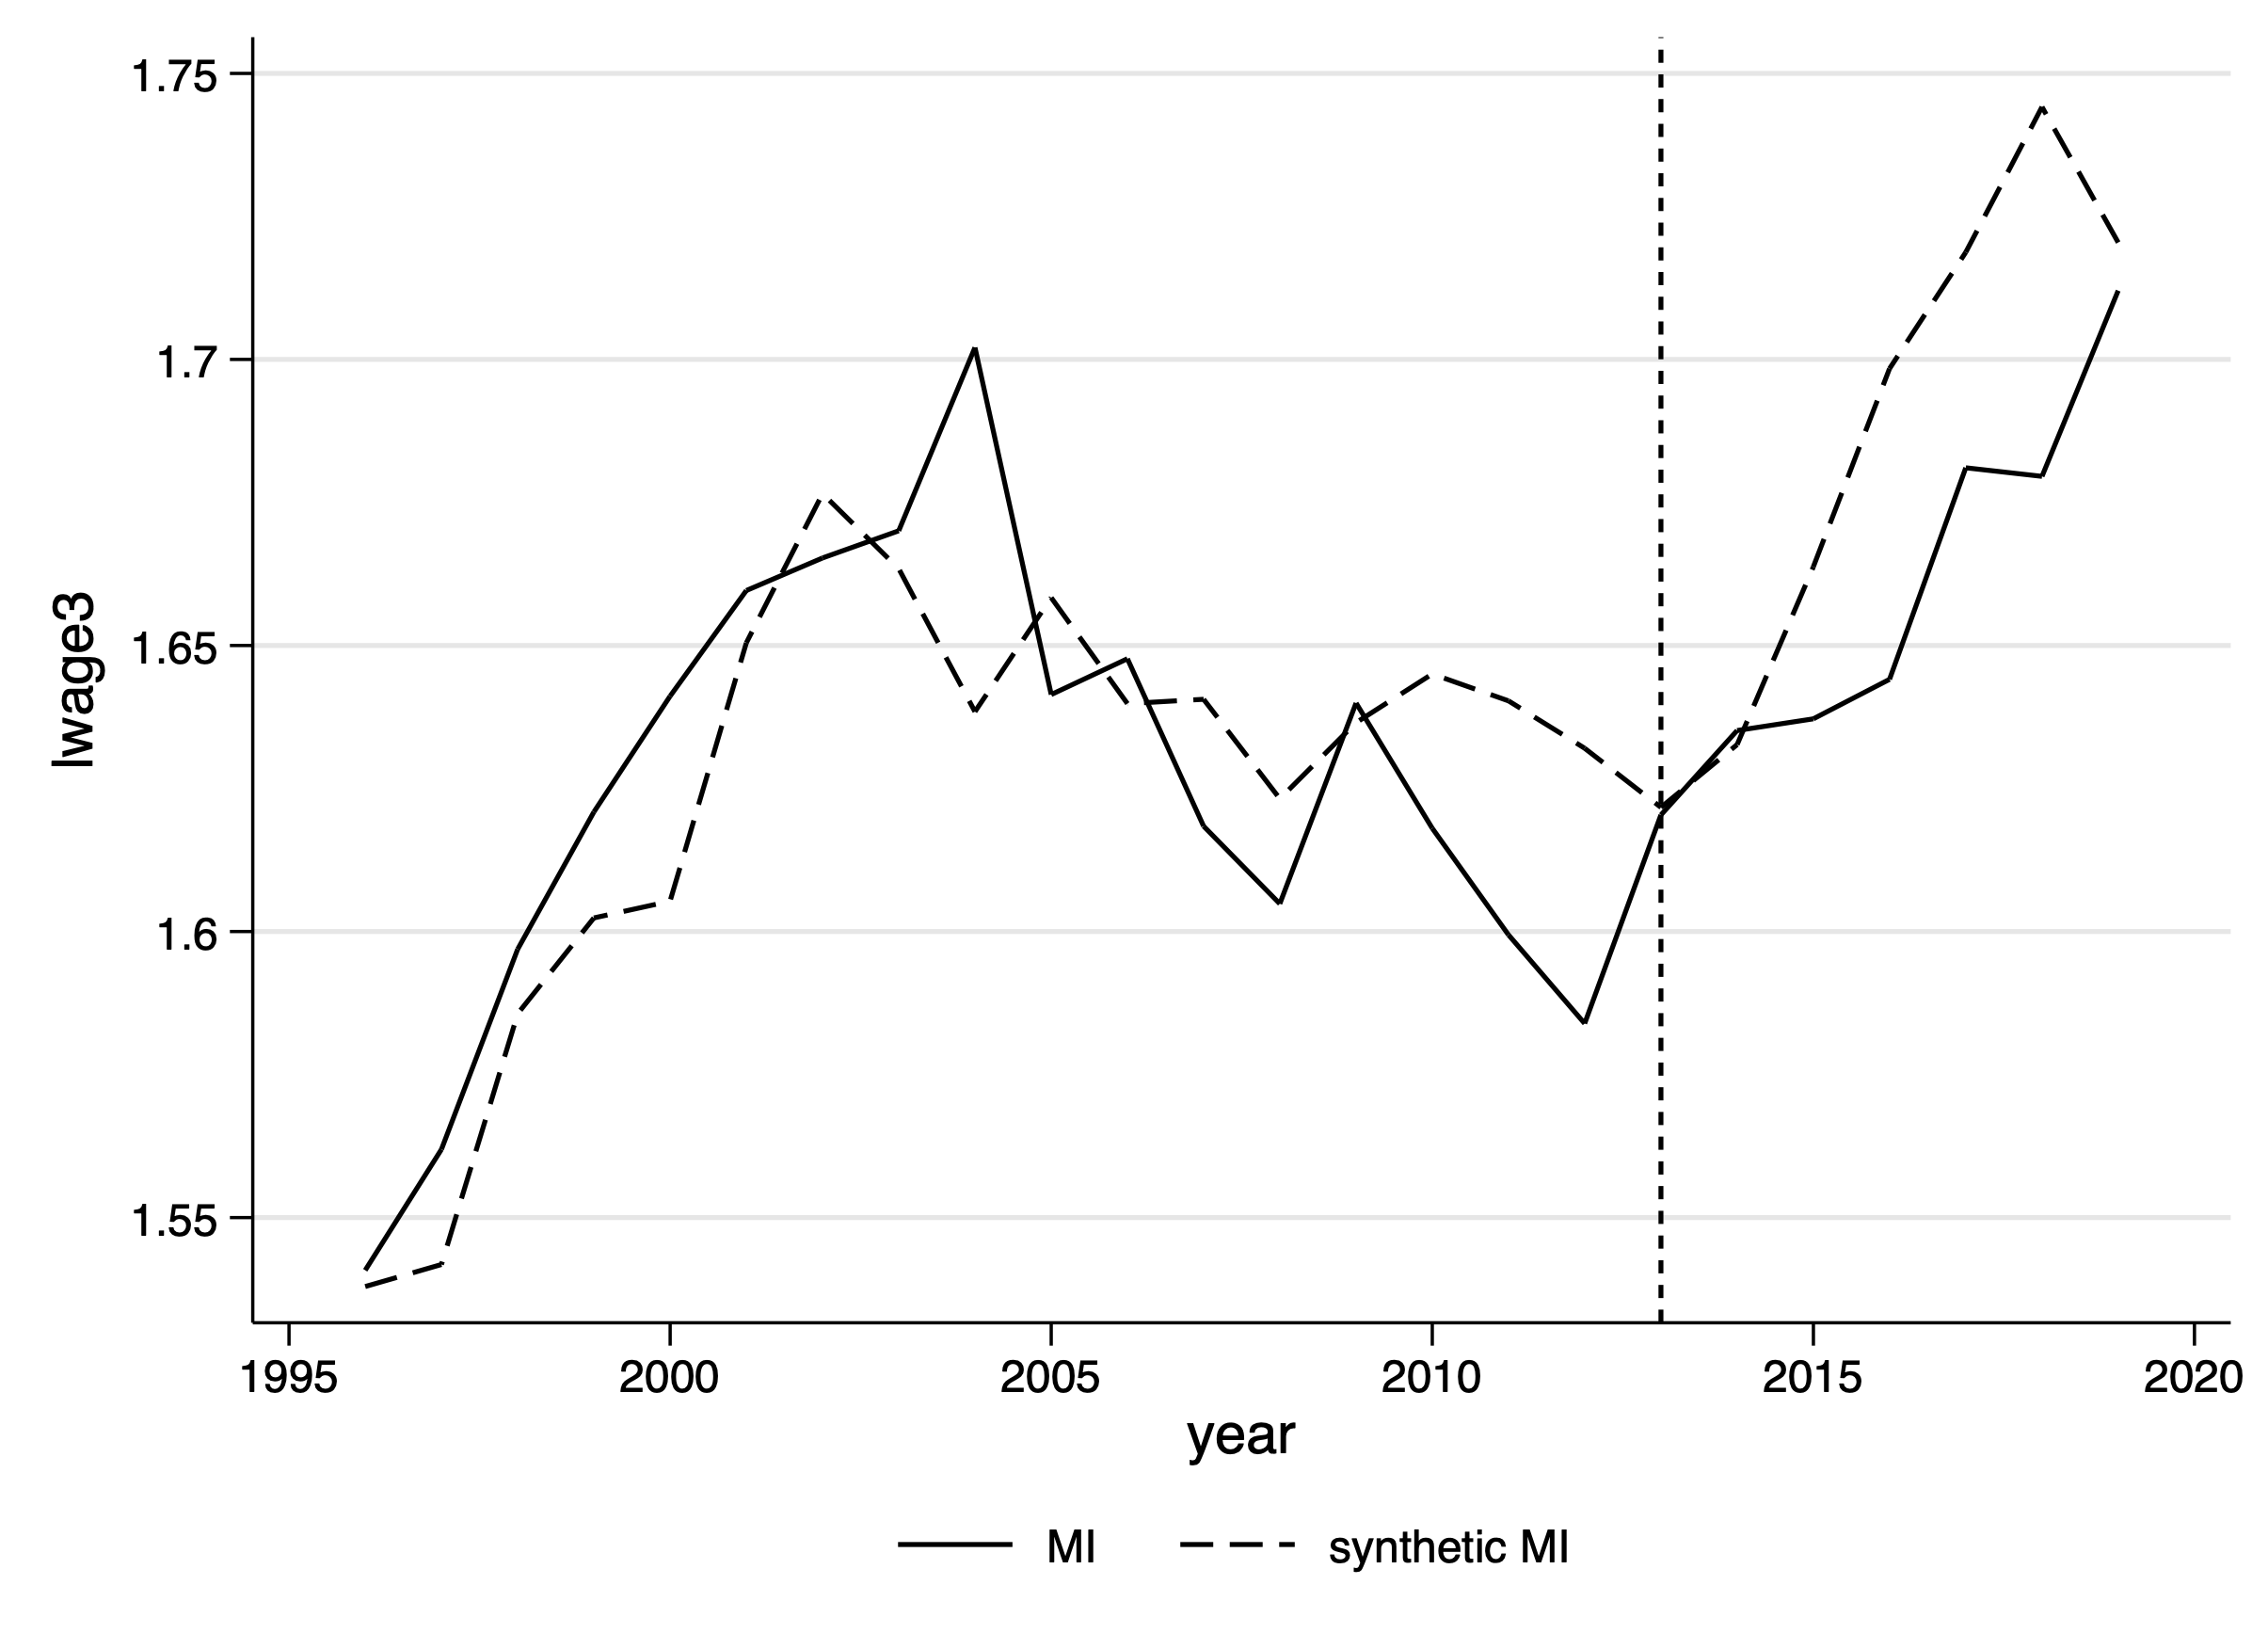
\includegraphics[width = 0.6\textwidth, keepaspectratio]{figures/fin_synth_wf_mi.png} & 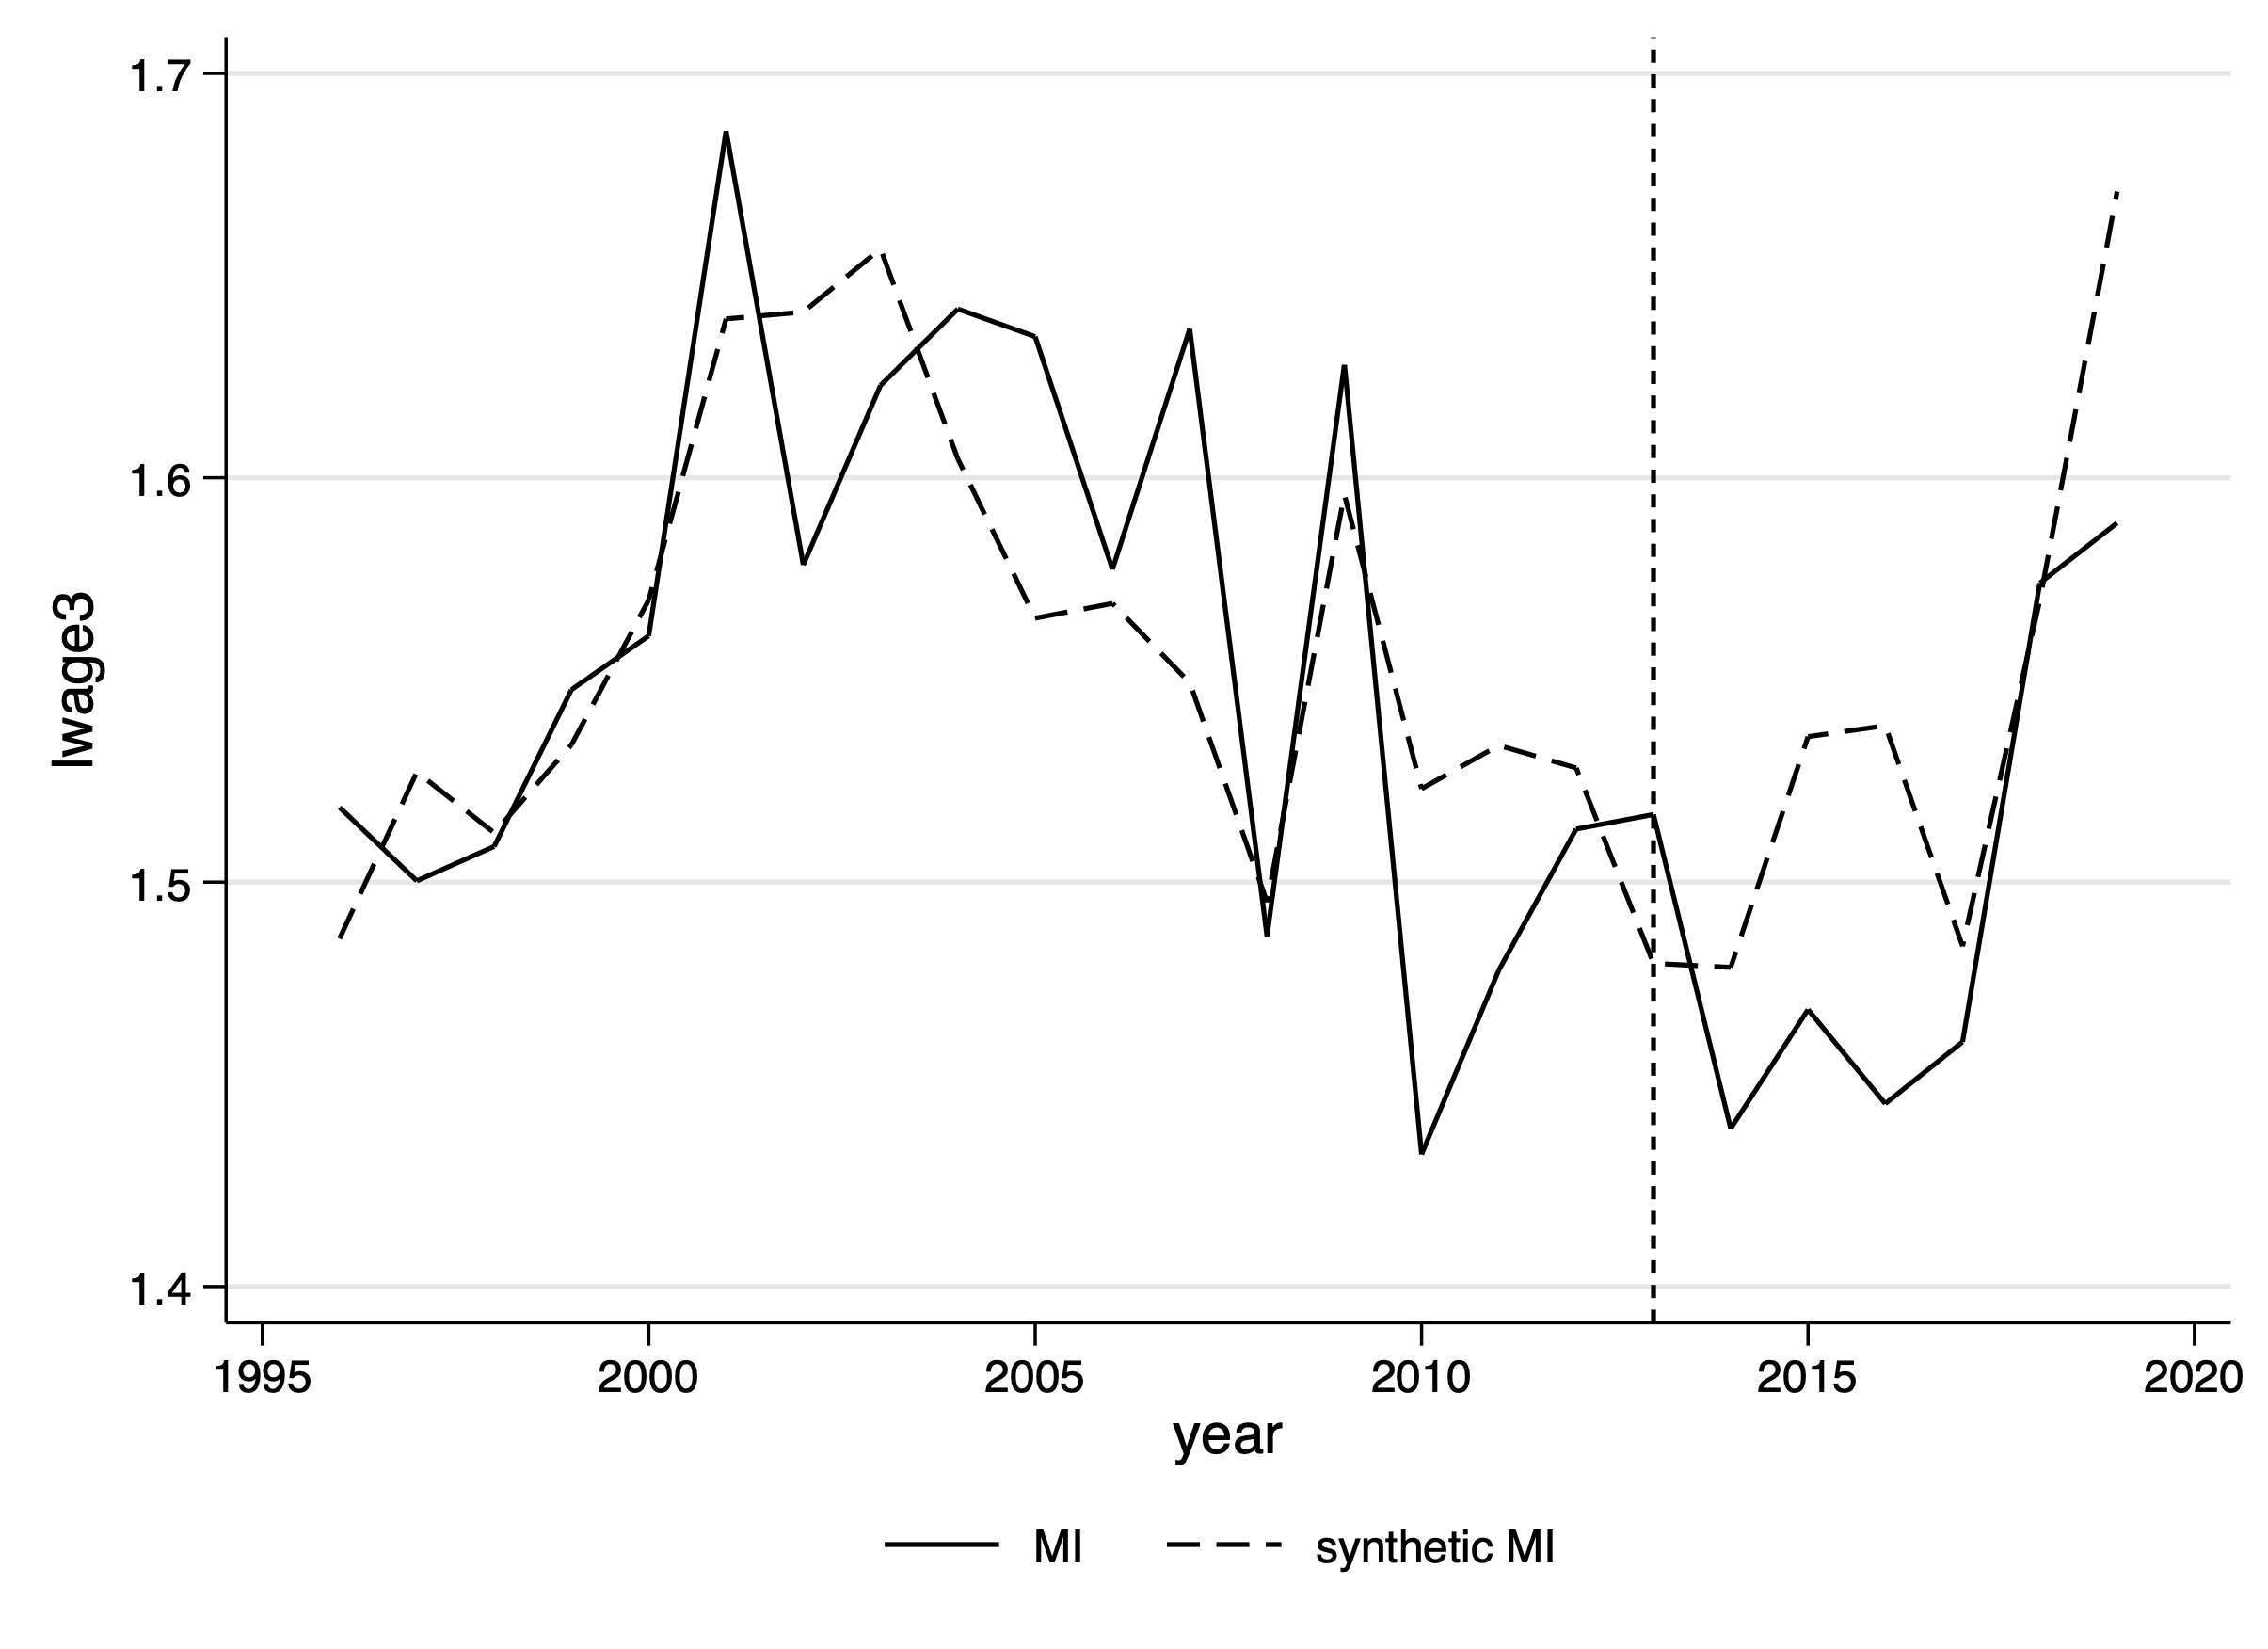
\includegraphics[width = 0.6\textwidth, keepaspectratio]{figures/fin_synth_bf_mi.png}
    \end{tabular}
\end{table}
% \footnotesize{Sample include years 1983-2019 excluding 1994 and 1995.}
\end{landscape}

\pagebreak
\begin{landscape}
\begin{table}[ht!]
    \centering
    \captionof{figure}{Synthetic Control Method - Wisconsin (2015)}\label{fig:synth_wi}
    \begin{tabular}{c c}
          \textbf{White Men} & \textbf{Black Men} \\    
          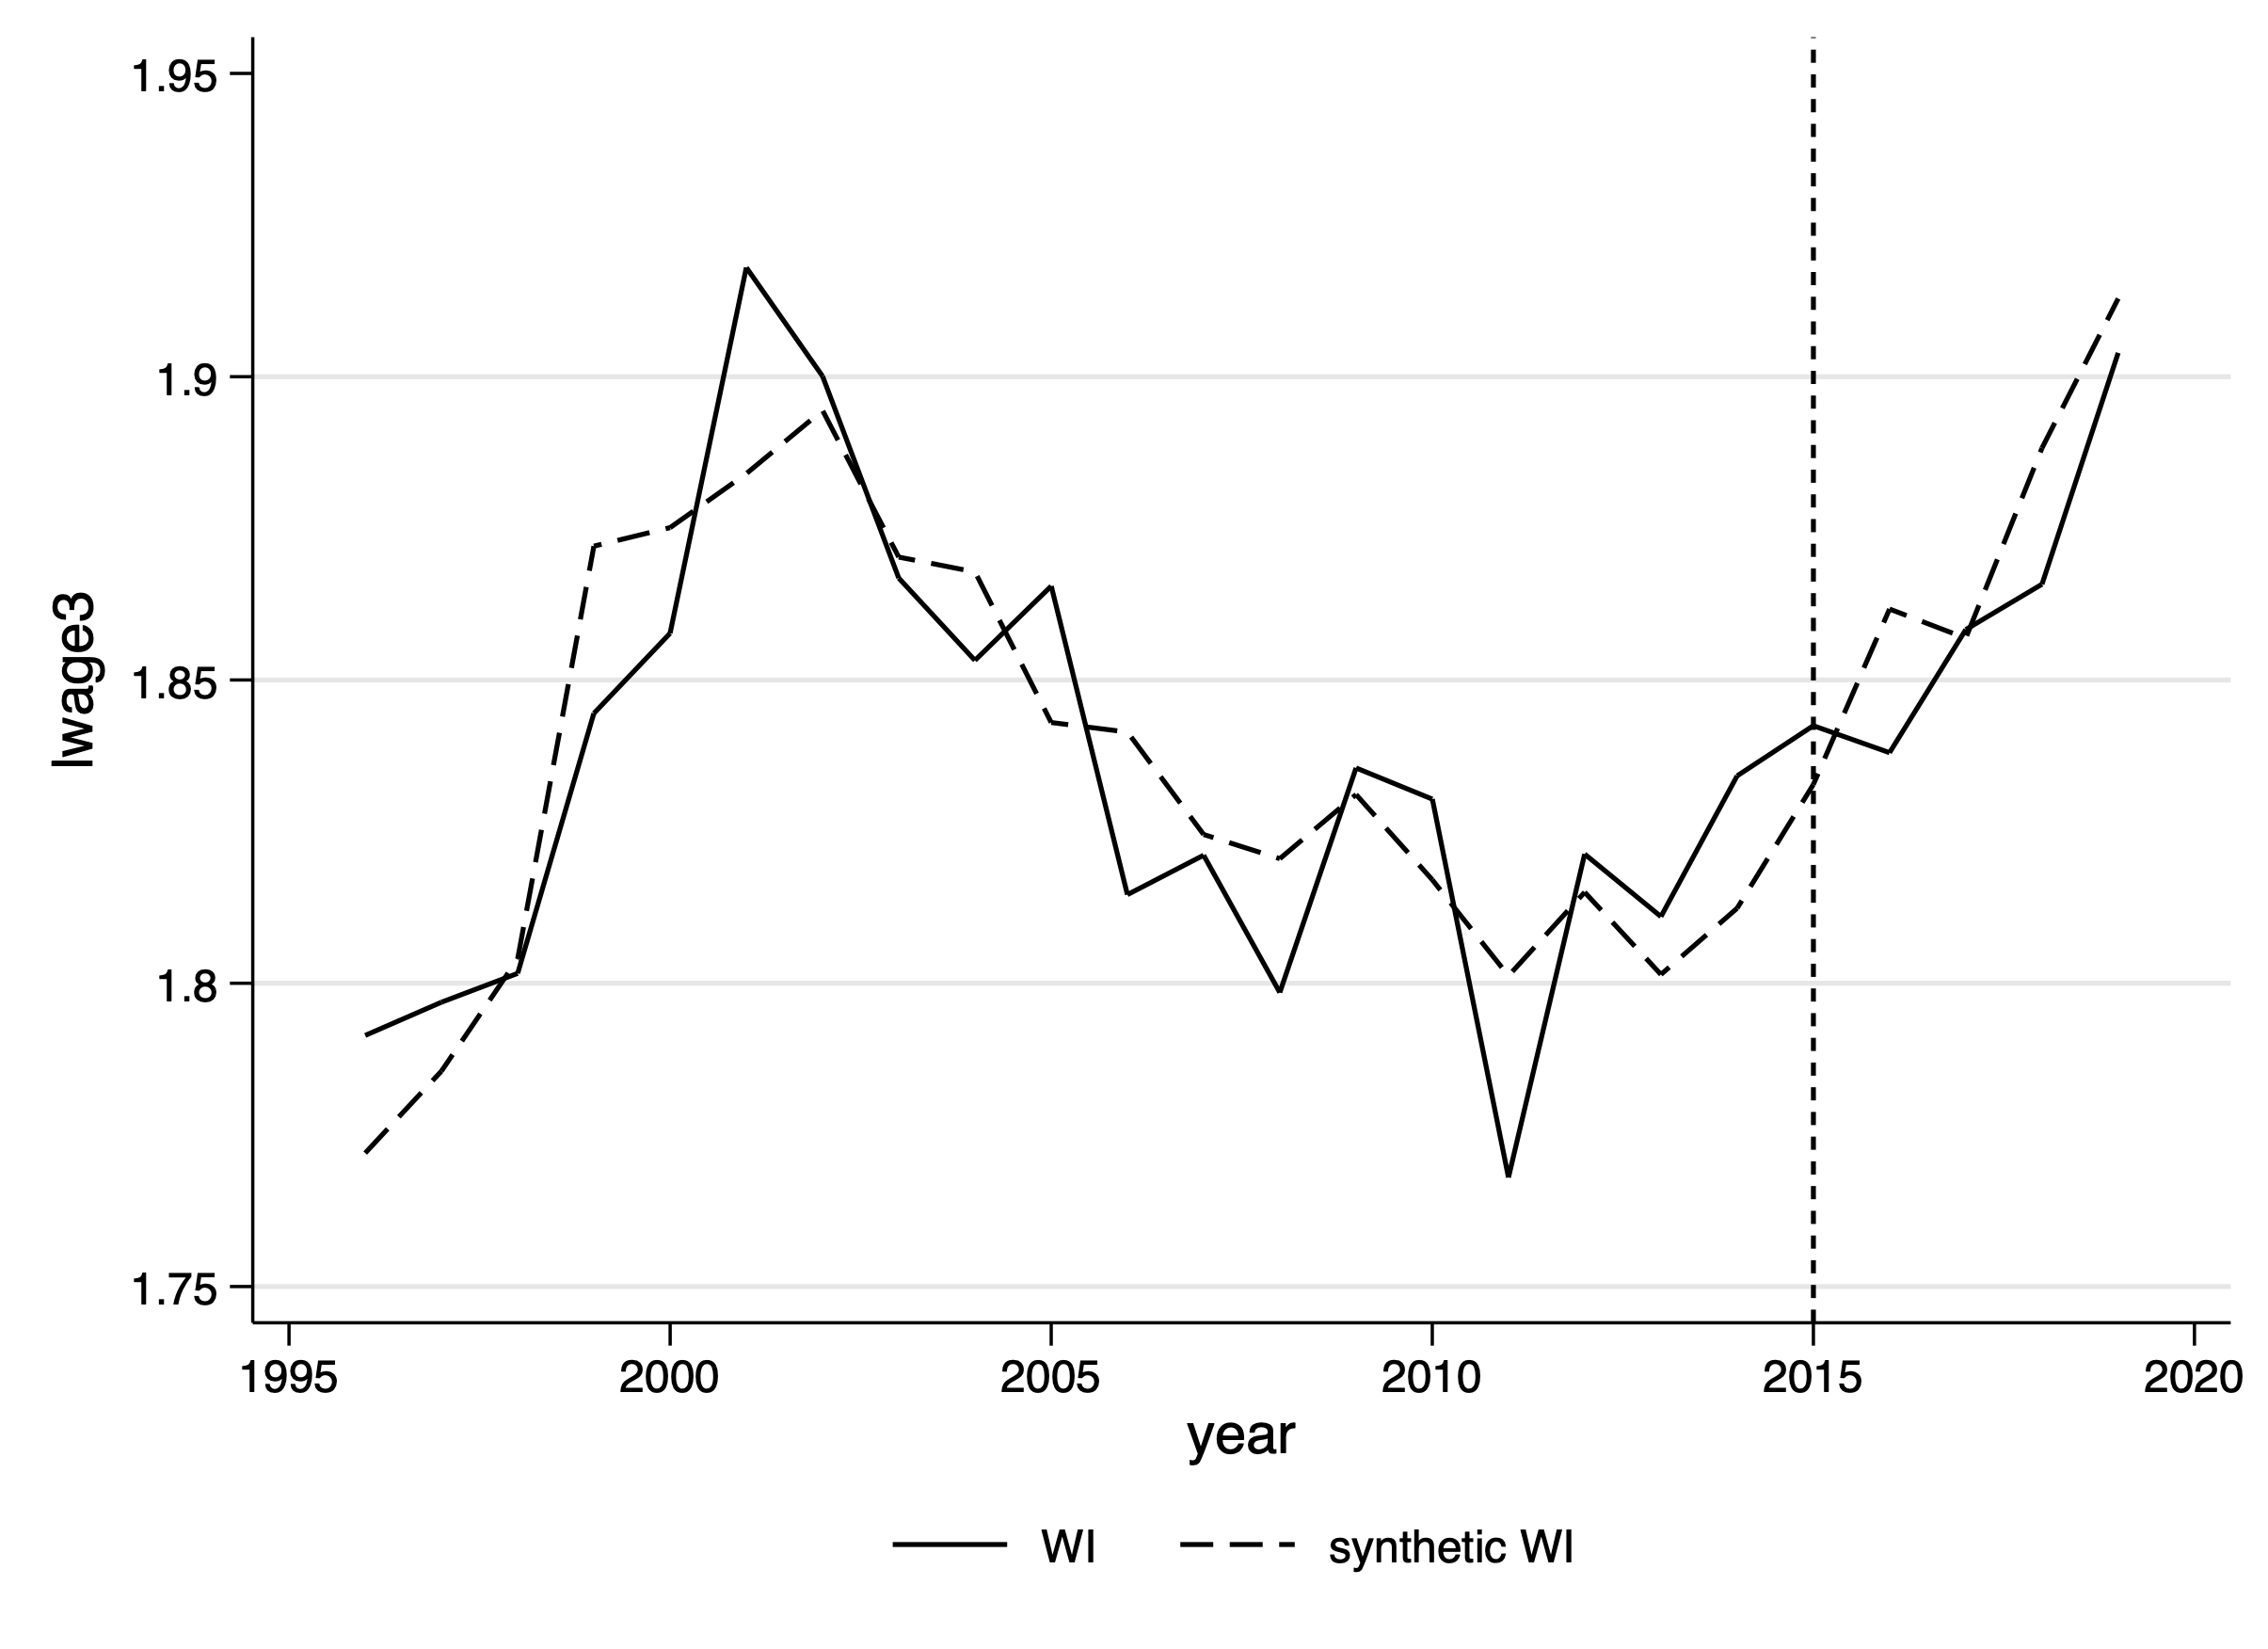
\includegraphics[width = 0.6\textwidth, keepaspectratio]{figures/fin_synth_wm_wi.png} & 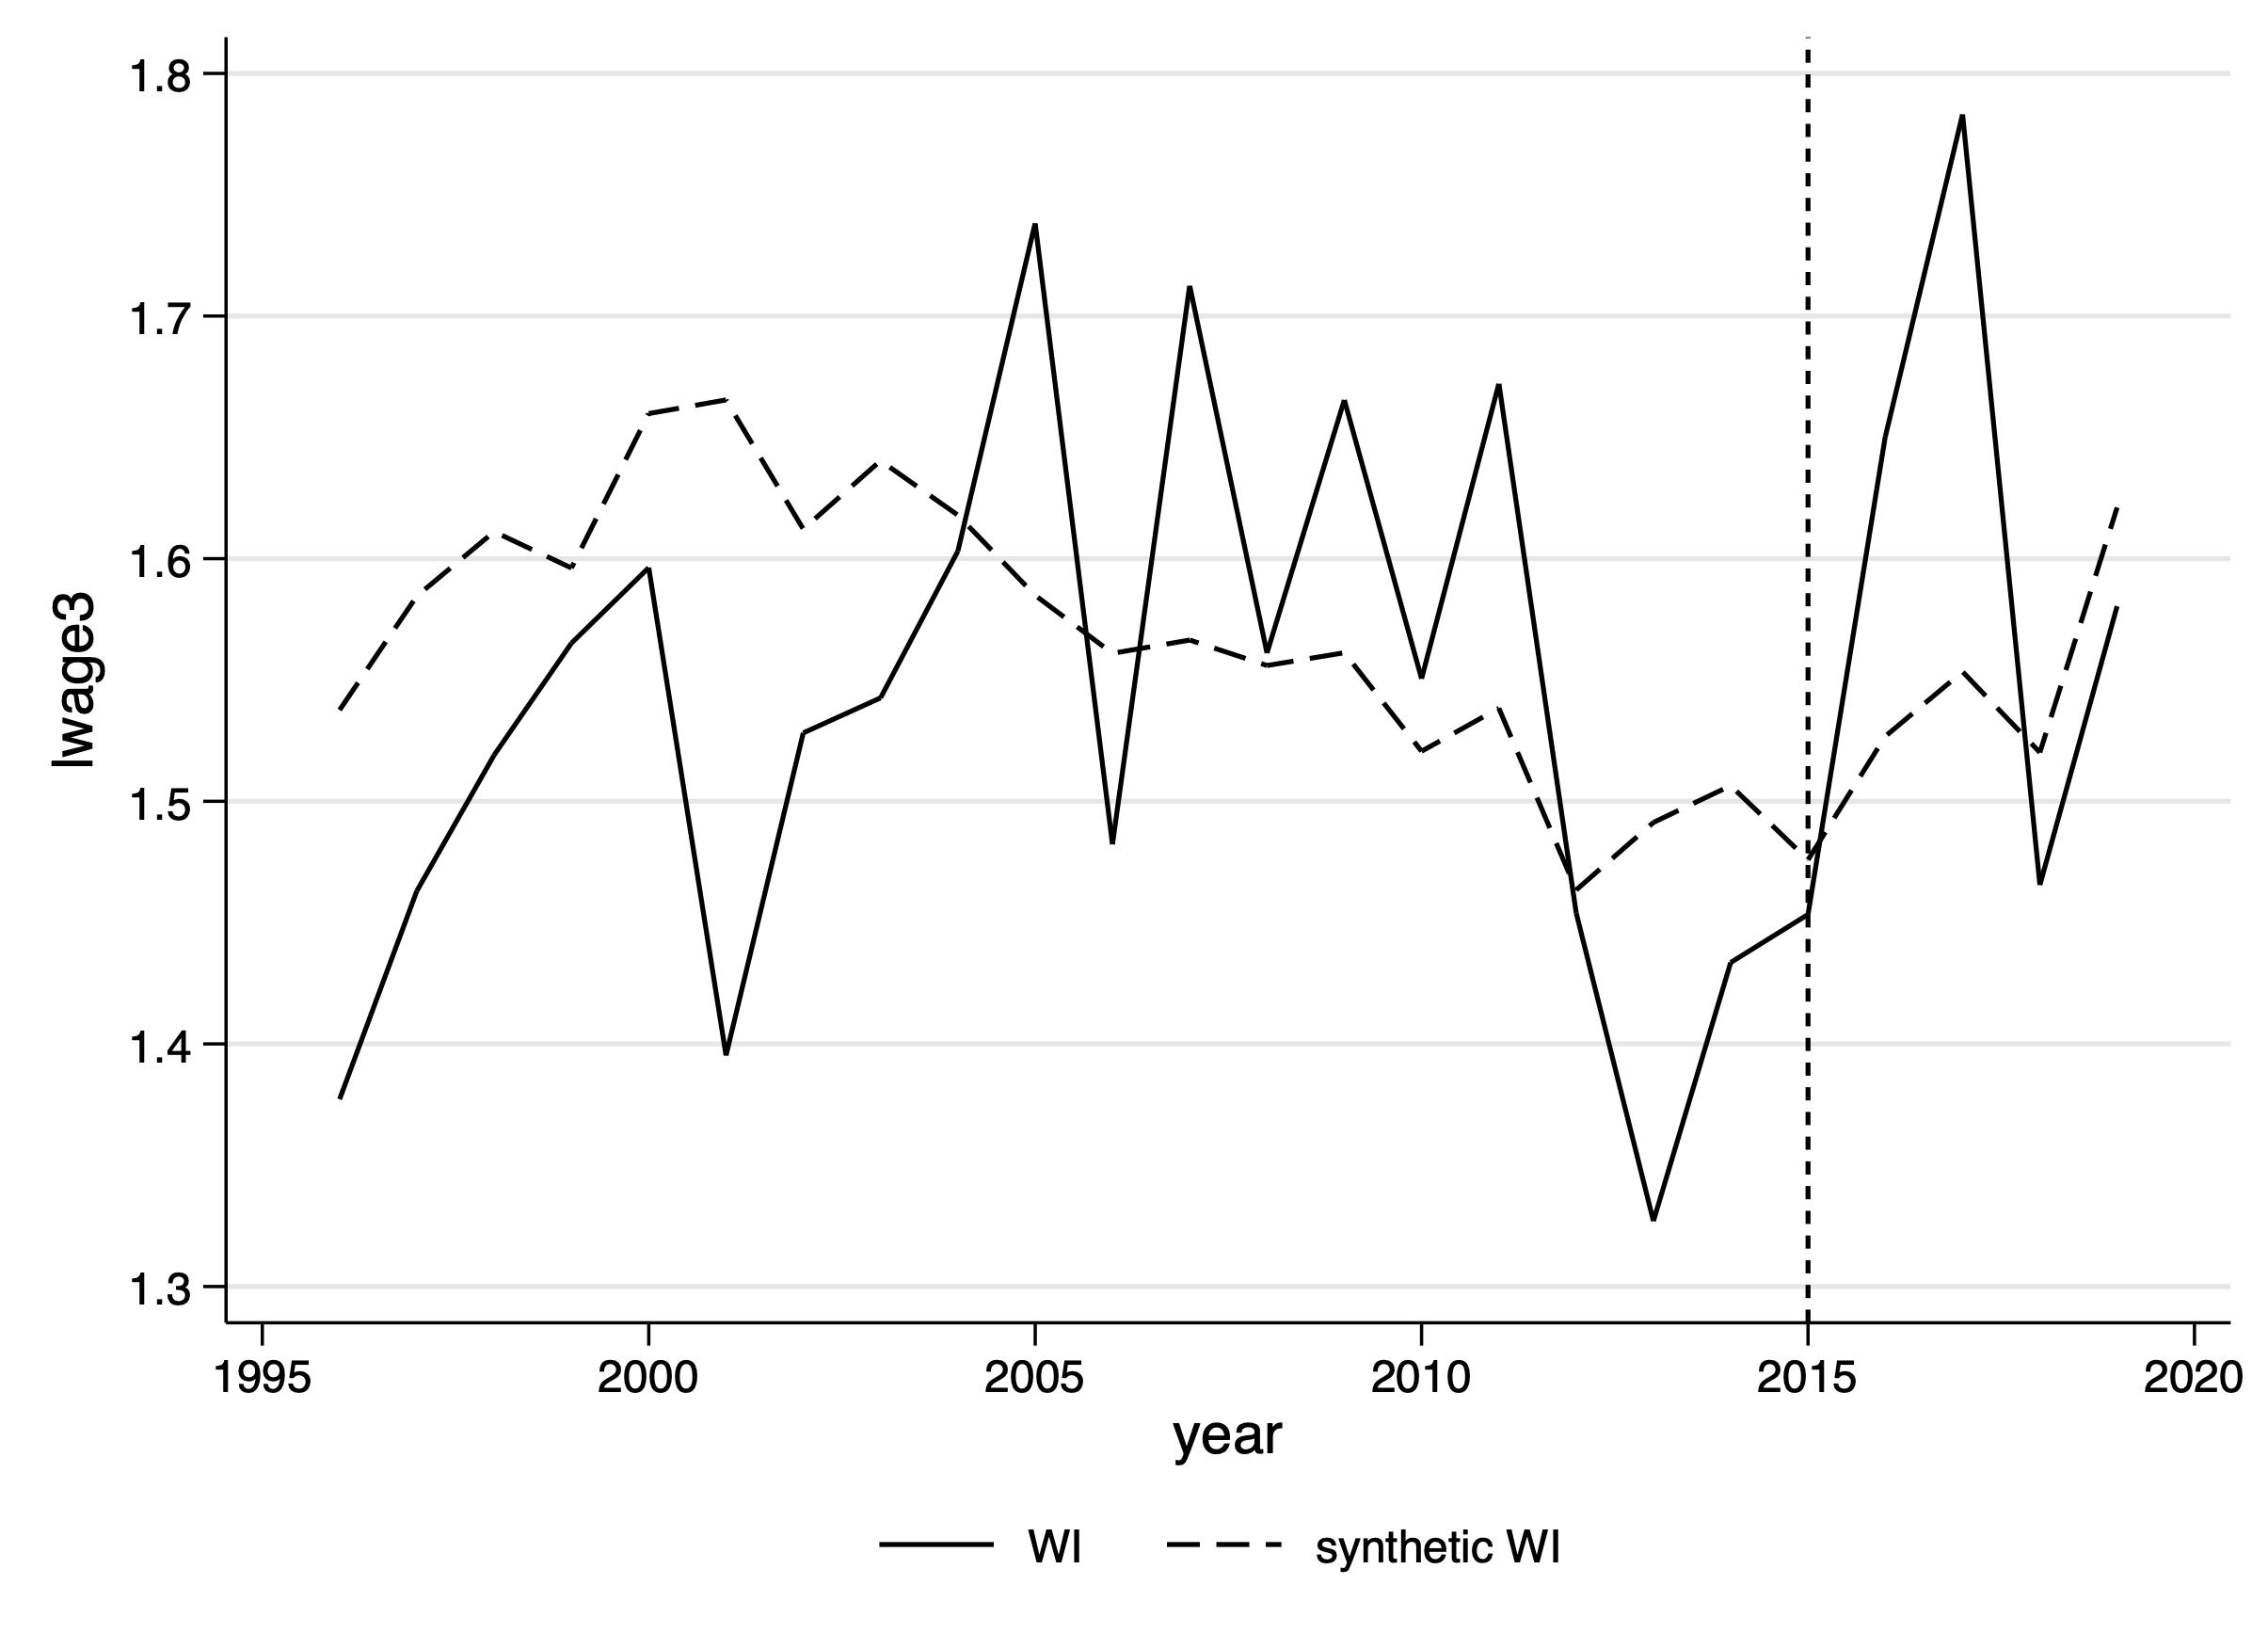
\includegraphics[width = 0.6\textwidth, keepaspectratio]{figures/fin_synth_bm_wi.png} \\
          \textbf{White Women} & \textbf{Black Women} \\
          \includegraphics[width = 0.6\textwidth, keepaspectratio]{figures/fin_synth_wf_wi.png} & \includegraphics[width = 0.6\textwidth, keepaspectratio]{figures/fin_synth_bf_wi.png}
    \end{tabular}
\end{table}
% \footnotesize{Sample include years 1983-2019 excluding 1994 and 1995.}
\end{landscape}

\pagebreak
\begin{landscape}
\begin{table}[ht!]
    \centering
    \captionof{figure}{Synthetic Control Method - Kentucky (2017)}\label{fig:synth_ky}
    \begin{tabular}{c c}
          \textbf{White Men} & \textbf{Black Men} \\    
          \includegraphics[width = 0.6\textwidth, keepaspectratio]{figures/fin_synth_wm_ky.png} & \includegraphics[width = 0.6\textwidth, keepaspectratio]{figures/fin_synth_bm_ky.png} \\
          \textbf{White Women} & \textbf{Black Women} \\
          \includegraphics[width = 0.6\textwidth, keepaspectratio]{figures/fin_synth_wf_ky.png} & \includegraphics[width = 0.6\textwidth, keepaspectratio]{figures/fin_synth_bf_ky.png}
    \end{tabular}
\end{table}
% \footnotesize{Sample include years 1983-2019 excluding 1994 and 1995.}
\end{landscape}

\pagebreak
\begin{landscape}
\section*{Tables}
\small{\begin{table}[h!]\centering
% \def\sym#1{\ifmmode^{#1}\else\(^{#1}\)\fi}
\caption{Summary Statistics by Hispanicity, Race, and Sex}\label{tab:bhw_sumstats}
\fontsize{10}{11}\selectfont
\begin{tabular}{l*{6}{c}}
\hline\hline
                    &\multicolumn{1}{c}{White Men}&\multicolumn{1}{c}{Black Men}&\multicolumn{1}{c}{Hispanic Men}&\multicolumn{1}{c}{White Women}&\multicolumn{1}{c}{Black Women}&\multicolumn{1}{c}{Hispanic Women}\\
\hline
Union Coverage      &       0.183&       0.225&       0.136&       0.137&       0.183&       0.125\\
                    &     (0.387)&     (0.418)&     (0.343)&     (0.344)&     (0.387)&     (0.331)\\
Union Membership    &       0.168&       0.203&       0.124&       0.119&       0.159&       0.109\\
                    &     (0.374)&     (0.402)&     (0.329)&     (0.324)&     (0.366)&     (0.312)\\
Real Log Wage (1979\$)&       1.874&       1.594&       1.507&       1.617&       1.480&       1.385\\
                    &     (0.595)&     (0.537)&     (0.515)&     (0.552)&     (0.519)&     (0.492)\\
Education           &      13.708&      12.933&      11.180&      13.813&      13.244&      12.050\\
                    &     (2.409)&     (2.331)&     (3.425)&     (2.282)&     (2.244)&     (3.111)\\
Experience          &      18.403&      18.118&      18.003&      18.442&      18.152&      17.683\\
                    &    (12.300)&    (12.039)&    (11.976)&    (12.638)&    (11.962)&    (12.345)\\
Public Sector       &       0.146&       0.187&       0.084&       0.195&       0.243&       0.153\\
                    &     (0.353)&     (0.390)&     (0.278)&     (0.397)&     (0.429)&     (0.360)\\
\hline
Observations        &     1609600&      150237&      209055&     1550943&      194743&      163809\\
\hline\hline
\multicolumn{7}{l}{\footnotesize Sample includes years 1983-2019 excluding 1994 and 1995.}\\
\end{tabular}
\end{table}
}
\end{landscape}

\pagebreak
\begin{landscape}
\small{\begin{table}[h!]
    \centering
    \caption{Percentage in each Industry by Hispanicity, Race, and Sex.}\label{tab:nindtab}
    \fontsize{10}{11}\selectfont
\begin{tabular}{l*{8}{c}}
 & \multicolumn{7}{c}{hispracesex} \\
nind&White Men&Black Men&Hispanic Men&White Women&Black Women&Hispanic Women&Total \\
&\%&\%&\%&\%&\%&\%&\% \\
\hline
Primary Sector&2.311&1.383&5.899&0.713&0.237&1.584&1.802 \\
Construction&9.360&5.809&15.908&1.283&0.469&0.988&5.735 \\
Manufacturing&20.337&18.044&16.926&8.978&9.120&12.031&14.631 \\
Wholesale and Retail Trade&20.625&21.416&24.557&20.878&18.279&26.258&21.261 \\
Transportation and Utilities&9.893&13.540&7.975&4.449&6.149&4.075&7.358 \\
Financial Services&5.285&4.202&3.351&8.473&7.041&6.507&6.423 \\
Business and Professional Services&12.608&11.608&12.177&10.457&8.521&9.894&11.335 \\
Health and Welfare Services&4.435&7.673&3.382&20.542&26.634&18.012&12.526 \\
Educational Services&6.488&6.087&3.357&15.446&11.807&10.305&10.045 \\
Personal Services&2.742&3.317&3.331&4.177&4.277&6.569&3.657 \\
Public Administration&5.917&6.922&3.137&4.606&7.467&3.776&5.228 \\
Total&100.000&100.000&100.000&100.000&100.000&100.000&100.000 \\

\hline\hline
\multicolumn{8}{l}{\footnotesize Sample includes years 1983-2019 excluding 1994 and 1995.}\\
\end{tabular}
\end{table}}
% \end{landscape}

% \pagebreak
% \begin{landscape}
\small{\begin{table}[h!]
    \centering
    \caption{Union Coverage Proportion in each Industry by Hispanicity, Race, and Sex.}\label{tab:unindtab}
    \fontsize{10}{11}\selectfont
\begin{tabular}{l*{8}{c}}
 & \multicolumn{7}{c}{hispracesex} \\
nind&White Men&Black Men&Hispanic Men&White Women&Black Women&Hispanic Women&Total \\
&Mean covered&Mean covered&Mean covered&Mean covered&Mean covered&Mean covered&Mean covered \\
\hline
Primary Sector&0.076&0.073&0.035&0.029&0.044&0.037&0.056 \\
Construction&0.234&0.208&0.107&0.060&0.157&0.053&0.188 \\
Manufacturing&0.184&0.252&0.145&0.101&0.183&0.105&0.162 \\
Wholesale and Retail Trade&0.060&0.077&0.066&0.046&0.057&0.053&0.056 \\
Transportation and Utilities&0.322&0.366&0.257&0.234&0.361&0.214&0.299 \\
Financial Services&0.030&0.091&0.081&0.021&0.055&0.035&0.032 \\
Business and Professional Services&0.042&0.081&0.059&0.022&0.054&0.051&0.039 \\
Health and Welfare Services&0.109&0.186&0.144&0.088&0.148&0.118&0.105 \\
Educational Services&0.379&0.356&0.348&0.429&0.383&0.367&0.405 \\
Personal Services&0.093&0.140&0.132&0.038&0.082&0.069&0.072 \\
Public Administration&0.412&0.396&0.454&0.305&0.329&0.350&0.369 \\
Total&0.169&0.206&0.125&0.134&0.171&0.121&0.152 \\

\hline\hline
\multicolumn{8}{l}{\footnotesize Sample includes years 1983-2019 excluding 1994 and 1995.}\\
\end{tabular}
\end{table}}
\end{landscape}

\pagebreak
\small{\begin{table}[h!]\centering
\def\sym#1{\ifmmode^{#1}\else\(^{#1}\)\fi}
\caption{OLS Regression of Real Log Wages on Union Coverage and Race}\label{tab:naive}
\fontsize{10}{11}\selectfont
\begin{tabular}{l*{2}{c}}
\hline
&\multicolumn{1}{c}{Men}&\multicolumn{1}{c}{Women}\\
\hline \multicolumn{3}{l}{ \linebreak \textbf{\textit{Panel A: 1983-1988}}} \\
$ Black $           &      -0.170***&     -0.0693***\\
&   (0.00549)   &   (0.00576)   \\
[1em]
$ covered $         &       0.190***&       0.173***\\
&    (0.0103)   &   (0.00845)   \\
[1em]
$ covered \times Black $&      0.0441***&      0.0160*  \\
&   (0.00979)   &   (0.00921)   \\
\hline
Observations        &      312495   &      286909   \\
\hline
\multicolumn{3}{l}{\linebreak \textbf{\textit{Panel B: 1988-2000}}} \\
$ Black $           &      -0.169***&     -0.0912***\\
&   (0.00418)   &   (0.00415)   \\
[1em]
$ covered $         &       0.179***&       0.151***\\
&   (0.00756)   &   (0.00640)   \\
[1em]
$ covered \times Black $&      0.0304***&      0.0336***\\
&   (0.00900)   &   (0.00905)   \\
\hline
Observations        &      524915   &      513808   \\
\hline
\multicolumn{3}{l}{\linebreak \textbf{\textit{Panel C: 2000-2019}}} \\
$ Black $           &      -0.163***&      -0.103***\\
&   (0.00350)   &   (0.00426)   \\
[1em]
$ covered $         &       0.171***&       0.120***\\
&   (0.00755)   &   (0.00700)   \\
[1em]
$ covered \times Black $&      0.0262***&      0.0405***\\
&   (0.00770)   &   (0.00806)   \\
\hline
Observations        &      628445   &      648645   \\
\hline\hline
\multicolumn{3}{l}{\footnotesize Standard errors in parentheses}\\
\multicolumn{3}{l}{\footnotesize * p<0.1, ** p<0.05, *** p<0.01}\\
\end{tabular}
\end{table}
}
\footnotesize{Standard errors are clustered at the state-industry level. Real log wages is the dependent variable throughout. Having the property of the coefficient in each panel is associated with a $ 100(e^\beta - 1) $ percent change in wages. Each column and panel corresponds to a regression. All regressions include covariates and fixed effects.}

\pagebreak
\small{\begin{table}[h!]\centering
\def\sym#1{\ifmmode^{#1}\else\(^{#1}\)\fi}
\caption{OLS of Real Log Wages on Unionization Rate for People Not Covered by Union}\label{tab:nlincovrate}
\begin{tabular}{l*{6}{c}}
\hline
&\multicolumn{3}{c}{Men}                        &\multicolumn{3}{c}{Women}                      \\\cmidrule(lr){2-4}\cmidrule(lr){5-7}
&\multicolumn{1}{c}{white}&\multicolumn{1}{c}{Black}&\multicolumn{1}{c}{Hispanic}&\multicolumn{1}{c}{White}&\multicolumn{1}{c}{Black}&\multicolumn{1}{c}{Hispanic}\\
\hline
\multicolumn{3}{l}{\linebreak \textbf{\textit{Panel A: 1983-1988}}} \\
$ coveragerate $    &       0.129***&      0.0713   &       0.263***&      0.0193   &      0.0460   &       0.130*  \\
&    (0.0408)   &    (0.0689)   &    (0.0659)   &    (0.0322)   &    (0.0608)   &    (0.0674)   \\
\hline
Observations        &      210643   &       20061   &       17369   &      211605   &       26249   &       13499   \\
\hline
\multicolumn{3}{l}{\linebreak \textbf{\textit{Panel B: 1988-2000}}} \\
$ coveragerate $    &       0.108***&      0.0893*  &       0.315***&      0.0227   &      0.0142   &       0.328***\\
&    (0.0280)   &    (0.0479)   &    (0.0666)   &    (0.0281)   &    (0.0465)   &    (0.0618)   \\
\hline
Observations        &      378776   &       35044   &       44952   &      386721   &       48587   &       34217   \\
\hline
\multicolumn{3}{l}{\linebreak \textbf{\textit{Panel C: 2000-2019}}} \\
$ coveragerate $    &      0.0682** &       0.109** &       0.255***&    -0.00995   &      0.0283   &       0.235***\\
&    (0.0300)   &    (0.0528)   &    (0.0554)   &    (0.0308)   &    (0.0429)   &    (0.0449)   \\
\hline
Observations        &      484955   &       47017   &       96726   &      493662   &       66038   &       77909   \\
\hline\hline
\multicolumn{7}{l}{\footnotesize Standard errors in parentheses}\\
\multicolumn{7}{l}{\footnotesize * p<0.1, ** p<0.05, *** p<0.01}\\
\end{tabular}
\end{table}
}
\footnotesize{Unionization rate is computed at the state-industry-year level. Standard errors are clustered at the state-industry level. Real log wages is the dependent variable throughout. A one percent increase in the unionization rate leads to a $100(e^{\beta} - 1)$ change in wages. Each column and panel corresponds to a regression. All regressions include covariates and fixed effects.}

\pagebreak
\begin{landscape}
\small{\begin{table}[htbp]\centering
\def\sym#1{\ifmmode^{#1}\else\(^{#1}\)\fi}
\caption{Difference in Differences of Real Log Wages on Right to Work Laws Treatment in State and Time}
\begin{tabular}{l*{6}{c}}
\hline
&\multicolumn{3}{c}{Men}                        &\multicolumn{3}{c}{Women}                      \\\cmidrule(lr){2-4}\cmidrule(lr){5-7}
&\multicolumn{1}{c}{(1)}   &\multicolumn{1}{c}{(2)}   &\multicolumn{1}{c}{(3)}   &\multicolumn{1}{c}{(4)}   &\multicolumn{1}{c}{(5)}   &\multicolumn{1}{c}{(6)}   \\
\hline
$ Black $           &      -0.144***&      -0.144***&      -0.145***&     -0.0663***&     -0.0663***&     -0.0672***\\
&   (0.00646)   &   (0.00647)   &   (0.00636)   &   (0.00657)   &   (0.00657)   &   (0.00651)   \\
[1em]
$ Treat\_{st} $      &     -0.0378** &     -0.0395** &     -0.0199*  &     -0.0317***&     -0.0325***&     -0.0572***\\
&    (0.0182)   &    (0.0190)   &    (0.0106)   &   (0.00833)   &   (0.00871)   &    (0.0117)   \\
[1em]
$ Treat\_{st} \times Black $&     -0.0221** &     -0.0221** &     -0.0220** &     -0.0397***&     -0.0397***&     -0.0389***\\
&   (0.00883)   &   (0.00886)   &   (0.00876)   &   (0.00800)   &   (0.00801)   &   (0.00807)   \\
\hline
Observations        &     1046468   &     1046468   &     1046468   &     1058304   &     1058304   &     1058304   \\
\hline
\end{table}
\multicolumn{3}{l}{\linebreak \textbf{\textit{Panel B: People Not Covered by Union - Spillover Effect}}} \\
$ Black $           &      -0.159***&      -0.159***&      -0.160***&     -0.0840***&     -0.0840***&     -0.0848***\\
&   (0.00502)   &   (0.00502)   &   (0.00497)   &   (0.00699)   &   (0.00699)   &   (0.00680)   \\
[1em]
$ Treat\_{st} $      &     -0.0266*  &     -0.0285*  &     -0.0199*  &     -0.0253***&     -0.0260***&     -0.0590***\\
&    (0.0136)   &    (0.0143)   &    (0.0114)   &   (0.00705)   &   (0.00726)   &    (0.0119)   \\
[1em]
$ Treat\_{st} \times Black $&    -0.00317   &    -0.00316   &    -0.00352   &     -0.0283***&     -0.0283***&     -0.0275***\\
&   (0.00811)   &   (0.00814)   &   (0.00820)   &   (0.00826)   &   (0.00827)   &   (0.00831)   \\
\hline
Observations        &      860332   &      860332   &      860332   &      905405   &      905405   &      905405   \\
\hline
\end{table}
\multicolumn{3}{l}{\linebreak \textbf{\textit{Panel C: People Covered by Union - Direct Effect}}} \\
$ Black $           &      -0.140***&      -0.140***&      -0.141***&     -0.0558***&     -0.0558***&     -0.0568***\\
&    (0.0123)   &    (0.0123)   &    (0.0122)   &    (0.0100)   &   (0.01000)   &   (0.00969)   \\
[1em]
$ Treat\_{st} $      &     -0.0575*  &     -0.0584*  &     -0.0471** &     -0.0608***&     -0.0616***&     -0.0539** \\
&    (0.0313)   &    (0.0322)   &    (0.0189)   &    (0.0184)   &    (0.0190)   &    (0.0213)   \\
[1em]
$ Treat\_{st} \times Black $&     -0.0146   &     -0.0146   &     -0.0135   &    0.000494   &    0.000540   &    0.000640   \\
&    (0.0147)   &    (0.0147)   &    (0.0145)   &    (0.0156)   &    (0.0156)   &    (0.0149)   \\
\hline
Observations        &      184674   &      184674   &      184674   &      151292   &      151292   &      151292   \\
State Monthly Unemployment Rate&          No   &         Yes   &         Yes   &          No   &         Yes   &         Yes   \\
Year Fixed Effect   &         Yes   &         Yes   &          No   &         Yes   &         Yes   &          No   \\
State Linear Time Trends&          No   &          No   &         Yes   &          No   &          No   &         Yes   \\
\hline\hline
\multicolumn{7}{l}{\footnotesize Standard errors in parentheses}\\
\multicolumn{7}{l}{\footnotesize * p<0.1, ** p<0.05, *** p<0.01}\\
\end{tabular}
\end{table}
}
\footnotesize{I define $RTW_{st} = 1$ if state $s$ has a RTW law at time $t$. Sample includes years 1983-2019. Policy variation: Oklahoma (2001), Indiana (2012), Michigan (2013), Wisconsin (2015), and Kentucky (2017). All states, except West Virginia, Montana, Maine, New Hampshire, and Vermont are in the sample. Standard errors are clustered at the state level. Real log wages is the dependent variable throughout. All regressions include covariates and fixed effects as outlined.}
\end{landscape}

\pagebreak
\section{Appendix - Tables and Figures}
\small{\begin{table}[h!]\centering
\def\sym#1{\ifmmode^{#1}\else\(^{#1}\)\fi}
\caption{OLS of Real Log Wages on Unionization Rate for People Covered by Union}\label{tab:ulincovrate}
\begin{tabular}{l*{6}{c}}
\hline
&\multicolumn{3}{c}{Men}                        &\multicolumn{3}{c}{Women}                      \\\cmidrule(lr){2-4}\cmidrule(lr){5-7}
&\multicolumn{1}{c}{white}&\multicolumn{1}{c}{Black}&\multicolumn{1}{c}{Hispanic}&\multicolumn{1}{c}{White}&\multicolumn{1}{c}{Black}&\multicolumn{1}{c}{Hispanic}\\
\hline
\multicolumn{3}{l}{\linebreak \textbf{\textit{Panel A: 1983-1988}}} \\
$ coveragerate $    &       0.319***&       0.413***&       0.586***&       0.343***&       0.420***&       0.418***\\
&    (0.0403)   &    (0.0829)   &     (0.136)   &    (0.0588)   &    (0.0919)   &     (0.160)   \\
\hline
Observations        &       72125   &        9666   &        5600   &       39825   &        9230   &        2950   \\
\hline
\multicolumn{3}{l}{\linebreak \textbf{\textit{Panel B: 1988-2000}}} \\
$ coveragerate $    &       0.286***&       0.335***&       0.566***&       0.224***&       0.358***&       0.515***\\
&    (0.0396)   &    (0.0495)   &    (0.0893)   &    (0.0563)   &    (0.0626)   &     (0.152)   \\
\hline
Observations        &       97722   &       13373   &        9306   &       64372   &       14128   &        5992   \\
\hline
\multicolumn{3}{l}{\linebreak \textbf{\textit{Panel C: 2000-2019}}} \\
$ coveragerate $    &       0.374***&       0.343***&       0.397***&       0.280***&       0.218***&       0.321***\\
&    (0.0419)   &    (0.0646)   &    (0.0949)   &    (0.0542)   &    (0.0668)   &     (0.121)   \\
\hline
Observations        &       85640   &       10833   &       12779   &       76061   &       12884   &       10446   \\
\hline\hline
\multicolumn{7}{l}{\footnotesize Standard errors in parentheses}\\
\multicolumn{7}{l}{\footnotesize * p<0.1, ** p<0.05, *** p<0.01}\\
\end{tabular}
\end{table}
}
\footnotesize{Unionization rate is computed at the state-industry-year level. Standard errors are clustered at the state-industry level. Real log wages is the dependent variable throughout. A one percent increase in the unionization rate leads to a $100(e^{\beta} - 1)$ change in wages. Each column and panel corresponds to a regression. All regressions include covariates and fixed effects.}

\pagebreak
\begin{landscape}
\small{\begin{table}[ht!]\centering
\def\sym#1{\ifmmode^{#1}\else\(^{#1}\)\fi}
\caption{Difference in Differences of Real Log Wages on Right to Work Laws in State and Time - W/O Always RTW States}
% \label{tab:wagstagdid-wo-ar2w}
\fontsize{10}{11}\selectfont
\begin{tabular}{l*{6}{c}}
\hline
&\multicolumn{3}{c}{Men}                        &\multicolumn{3}{c}{Women}                      \\\cmidrule(lr){2-4}\cmidrule(lr){5-7}
&\multicolumn{1}{c}{(1)}   &\multicolumn{1}{c}{(2)}   &\multicolumn{1}{c}{(3)}   &\multicolumn{1}{c}{(4)}   &\multicolumn{1}{c}{(5)}   &\multicolumn{1}{c}{(6)}   \\
\hline
\multicolumn{3}{l}{\linebreak \textbf{\textit{Panel A: All (Black and White) People}}} \\
$ Black $           &      -0.144***&      -0.144***&      -0.145***&     -0.0671***&     -0.0671***&     -0.0679***\\
&   (0.00671)   &   (0.00672)   &   (0.00660)   &   (0.00661)   &   (0.00661)   &   (0.00653)   \\
[1em]
$ RTW_{st} $      &     -0.0348*  &     -0.0360*  &     -0.0215*  &     -0.0372***&     -0.0374***&     -0.0590***\\
&    (0.0187)   &    (0.0194)   &    (0.0111)   &   (0.00864)   &   (0.00898)   &    (0.0121)   \\
[1em]
$ RTW_{st} \times Black $&     -0.0110   &     -0.0112   &    -0.00686   &     -0.0165** &     -0.0165** &     -0.0141** \\
&   (0.00760)   &   (0.00774)   &   (0.00702)   &   (0.00751)   &   (0.00754)   &   (0.00681)   \\
\hline
Observations        &      613198   &      613198   &      613198   &      618164   &      618164   &      618164   \\
\hline
\multicolumn{3}{l}{\linebreak \textbf{\textit{Panel B: People Not Covered by Union - Spillover Effect}}} \\
$ Black $           &      -0.156***&      -0.156***&      -0.157***&     -0.0849***&     -0.0849***&     -0.0854***\\
&   (0.00507)   &   (0.00506)   &   (0.00501)   &   (0.00709)   &   (0.00709)   &   (0.00688)   \\
[1em]
$ RTW_{st} $      &     -0.0255*  &     -0.0267*  &     -0.0214*  &     -0.0326***&     -0.0327***&     -0.0600***\\
&    (0.0144)   &    (0.0151)   &    (0.0119)   &   (0.00732)   &   (0.00763)   &    (0.0121)   \\
[1em]
$ RTW_{st} \times Black $&     0.00298   &     0.00274   &     0.00542   &     -0.0166*  &     -0.0166*  &     -0.0160*  \\
&   (0.00693)   &   (0.00697)   &   (0.00729)   &   (0.00872)   &   (0.00876)   &   (0.00804)   \\
\hline
Observations        &      475638   &      475638   &      475638   &      505518   &      505518   &      505518   \\
\hline
\multicolumn{3}{l}{\linebreak \textbf{\textit{Panel C: People Covered by Union - Direct Effect}}} \\
$ Black $           &      -0.137***&      -0.137***&      -0.138***&     -0.0494***&     -0.0494***&     -0.0505***\\
&    (0.0124)   &    (0.0124)   &    (0.0123)   &    (0.0100)   &    (0.0100)   &   (0.00969)   \\
[1em]
$ RTW_{st} $      &     -0.0551*  &     -0.0559*  &     -0.0451** &     -0.0708***&     -0.0714***&     -0.0600** \\
&    (0.0312)   &    (0.0321)   &    (0.0197)   &    (0.0170)   &    (0.0176)   &    (0.0218)   \\
[1em]
$ RTW_{st} \times Black $&     -0.0235   &     -0.0235   &     -0.0153   &      0.0417   &      0.0416   &      0.0478   \\
&    (0.0188)   &    (0.0188)   &    (0.0173)   &    (0.0279)   &    (0.0279)   &    (0.0290)   \\
\hline
Observations        &      136489   &      136489   &      136489   &      111486   &      111486   &      111486   \\
State Monthly Unemployment Rate&          No   &         Yes   &         Yes   &          No   &         Yes   &         Yes   \\
Year Fixed Effect   &         Yes   &         Yes   &          No   &         Yes   &         Yes   &          No   \\
State Linear Time Trends&          No   &          No   &         Yes   &          No   &          No   &         Yes   \\
\hline\hline
\multicolumn{7}{l}{\footnotesize Standard errors in parentheses}\\
\multicolumn{7}{l}{\footnotesize * p<0.1, ** p<0.05, *** p<0.01}\\
\end{tabular}
\end{table}
}
\footnotesize{I define $RTW_{st} = 1$ if state $s$ has a RTW law at time $t$. Sample includes years 1983-2019. Policy variation: Oklahoma (2001), Indiana (2012), Michigan (2013), Wisconsin (2015), and Kentucky (2017). All states, except West Virginia, Montana, Maine, New Hampshire, and Vermont are in the sample. Standard errors are clustered at the state level. Real log wages is the dependent variable throughout. All regressions include covariates and fixed effects as outlined.}
\end{landscape}

\pagebreak
\begin{landscape}
\begin{figure}[ht!]
\centering
    \caption{RIF-DID Regression of Real Log Wages on Right to Work Laws Treatment in State and Time - People Covered by Union - Direct Effect}\label{fig:rifdid-sltt-C}
    \includegraphics[width=1.25\textwidth, height = \textheight, keepaspectratio]{figures/fin_rifdid-sltt-C.png}
\end{figure}
\footnotesize{I define $RTW_{st} = 1$ if state $s$ has a RTW law at time $t$. Sample includes years 1983-2019. Policy variation: Oklahoma (2001), Indiana (2012), Michigan (2013), Wisconsin (2015), and Kentucky (2017). All states, except West Virginia, Montana, Maine, New Hampshire, and Vermont are in the sample. Standard errors for the DID regression are clustered at the state level. Standard errors for the RIF-DID regression are bootstrapped with 100 replicates. Real log wages is the dependent variable throughout. Each column corresponds to a regression and associated set of RIF-DID regressions. 95\% confidence intervals presented. All regressions include covariates and fixed effects as outlined. State monthly unemployment rate and state linear time trends included. Year fixed effects not included.}
\end{landscape}

\pagebreak
\begin{landscape}
\begin{figure}[ht!]
\centering
    \caption{RIF-DID Regression of Real Log Wages on Right to Work Laws Treatment in State and Time - All (Black and White) People - W/O Always RTW States}\label{fig:rifdid-sltt-wo-ar2w-A}
    \includegraphics[width=1.25\textwidth, height = \textheight, keepaspectratio]{figures/fin_rifdid-sltt-wo-ar2w-A.png}
\end{figure}
\footnotesize{I define $RTW_{st} = 1$ if state $s$ has a RTW law at time $t$. Sample includes years 1983-2019. Policy variation: Oklahoma (2001), Indiana (2012), Michigan (2013), Wisconsin (2015), and Kentucky (2017). All states, except West Virginia, Montana, Maine, New Hampshire, and Vermont are in the sample. Standard errors for the DID regression are clustered at the state level. Standard errors for the RIF-DID regression are bootstrapped with 100 replicates. Real log wages is the dependent variable throughout. Each column corresponds to a regression and associated set of RIF-DID regressions. 95\% confidence intervals presented. All regressions include covariates and fixed effects as outlined. State monthly unemployment rate and state linear time trends included. Year fixed effects not included.}
\end{landscape}

\pagebreak
\begin{landscape}
\begin{figure}[ht!]
\centering
    \caption{RIF-DID Regression of Real Log Wages on Right to Work Laws Treatment in State and Time - People Not Covered by Union - Spillover Effect - W/O Always RTW States}\label{fig:rifdid-sltt-wo-ar2w-B}
    \includegraphics[width=1.25\textwidth, height = \textheight, keepaspectratio]{figures/fin_rifdid-sltt-wo-ar2w-B.png}
\end{figure}
\footnotesize{I define $RTW_{st} = 1$ if state $s$ has a RTW law at time $t$. Sample includes years 1983-2019. Policy variation: Oklahoma (2001), Indiana (2012), Michigan (2013), Wisconsin (2015), and Kentucky (2017). All states, except West Virginia, Montana, Maine, New Hampshire, and Vermont are in the sample. Standard errors for the DID regression are clustered at the state level. Standard errors for the RIF-DID regression are bootstrapped with 100 replicates. Real log wages is the dependent variable throughout. Each column corresponds to a regression and associated set of RIF-DID regressions. 95\% confidence intervals presented. All regressions include covariates and fixed effects as outlined. State monthly unemployment rate and state linear time trends included. Year fixed effects not included.}
\end{landscape}

\pagebreak
\begin{landscape}
\begin{figure}[ht!]
\centering
    \caption{RIF-DID Regression of Real Log Wages on Right to Work Laws Treatment in State and Time - People Covered by Union - Direct Effect - W/O Always RTW States}\label{fig:rifdid-sltt-wo-ar2w-C}
    \includegraphics[width=1.25\textwidth, height = \textheight, keepaspectratio]{figures/fin_rifdid-sltt-wo-ar2w-C.png}
\end{figure}
\footnotesize{I define $RTW_{st} = 1$ if state $s$ has a RTW law at time $t$. Sample includes years 1983-2019. Policy variation: Oklahoma (2001), Indiana (2012), Michigan (2013), Wisconsin (2015), and Kentucky (2017). All states, except West Virginia, Montana, Maine, New Hampshire, and Vermont are in the sample. Standard errors for the DID regression are clustered at the state level. Standard errors for the RIF-DID regression are bootstrapped with 100 replicates. Real log wages is the dependent variable throughout. Each column corresponds to a regression and associated set of RIF-DID regressions. 95\% confidence intervals presented. All regressions include covariates and fixed effects as outlined. State monthly unemployment rate and state linear time trends included. Year fixed effects not included.}
\end{landscape}

\pagebreak
\begin{landscape}
\begin{table}[h!]
    \centering
    \captionof{figure}{Predicted Real Log Wage Trends - West Virginia (2016)}\label{fig:pta_wv}
    \begin{tabular}{c c}
          \includegraphics[width = 0.6\textwidth, keepaspectratio]{figures/pta/fin_wm_wv.png} & \includegraphics[width = 0.6\textwidth, keepaspectratio]{figures/pta/fin_bm_wv.png} \\
          \includegraphics[width = 0.6\textwidth, keepaspectratio]{figures/pta/fin_wf_wv.png} & \includegraphics[width = 0.6\textwidth, keepaspectratio]{figures/pta/fin_bf_wv.png}
    \end{tabular}
\end{table}
% \footnotesize{Sample include years 1983-2019 excluding 1994 and 1995.}
\end{landscape}

\pagebreak
\small{\begin{table}[ht!]\centering
\caption{Synthetic Control Method - Weights Assigned to Donor States - White Men}\label{tab:donor_weights_wm}
\fontsize{10}{11}\selectfont
\begin{tabular}{llllll}
            &                 &                &                 &                  &                 \\
            \hline
            \hline
            & Oklahoma (2001) & Indiana (2012) & Michigan (2013) & Wisconsin (2015) & Kentucky (2017) \\
            \hline
Donor State & Unit Weight     & Unit Weight    & Unit Weight     & Unit Weight      & Unit Weight     \\
            \hline
ME          & 0.3             & 0              & 0               & 0.179            & 0               \\
NH          & 0               & 0              & 0               & 0                & 0               \\
VT          & 0.262           & 0              & 0               & 0                & 0               \\
MA          & 0               & 0              & 0               & 0                & 0               \\
RI          & 0               & 0              & 0               & 0                & 0               \\
CT          & 0               & 0              & 0               & 0                & 0               \\
NY          & 0               & 0              & 0               & 0                & 0               \\
NJ          & 0               & 0              & 0               & 0                & 0               \\
PA          & 0               & 0.24           & 0               & 0                & 0               \\
OH          & 0               & 0.559          & 0.887           & 0.6              & 0.24            \\
IL          & 0               & 0              & 0               & 0                & 0               \\
MN          & 0               & 0              & 0               & 0.197            & 0               \\
MO          & 0.117           & 0.107          & 0               & 0                & 0.223           \\
DE          & 0               & 0              & 0               & 0                & 0               \\
MD          & 0               & 0              & 0               & 0                & 0               \\
DC          & 0               & 0              & 0.113           & 0.024            & 0               \\
MT          & 0.14            & 0.093          & 0               & 0                & 0.536           \\
CO          & 0               & 0              & 0               & 0                & 0               \\
NM          & 0.181           & 0              & 0               & 0                & 0               \\
WA          & 0               & 0              & 0               & 0                & 0               \\
OR          & 0               & 0              & 0               & 0                & 0               \\
CA          & 0               & 0              & 0               & 0                & 0               \\
AK          & 0               & 0              & 0               & 0                & 0               \\
HI          & 0               & 0              & 0               & 0                & 0\\
\hline
\end{tabular}
\end{table}}

\pagebreak
\small{\begin{table}[ht!]\centering
\caption{Synthetic Control Method - Weights Assigned to Donor States - Black Men}\label{tab:donor_weights_bm}
\fontsize{10}{11}\selectfont
\begin{tabular}{llllll}
            &                 &                &                 &                  &                 \\
            \hline
            \hline
            & Oklahoma (2001) & Indiana (2012) & Michigan (2013) & Wisconsin (2015) & Kentucky (2017) \\
            \hline
Donor State & Unit Weight     & Unit Weight    & Unit Weight     & Unit Weight      & Unit Weight     \\
            \hline
ME          & -               & -              & -               & -                & -               \\
NH          & -               & -              & -               & -                & -               \\
VT          & -               & -              & -               & -                & -               \\
MA          & 0               & 0.043          & 0.034           & 0                & 0               \\
RI          & 0               & 0.109          & 0.354           & 0.167            & 0               \\
CT          & 0               & 0              & 0               & 0                & 0               \\
NY          & 0               & 0              & 0               & 0                & 0               \\
NJ          & 0               & 0              & 0.04            & 0                & 0               \\
PA          & 0               & 0              & 0               & 0.065            & 0.151           \\
OH          & 0.709           & 0.43           & 0.002           & 0.768            & 0.774           \\
IL          & 0               & 0              & 0               & 0                & 0               \\
MN          & 0               & 0              & 0               & 0                & 0               \\
MO          & 0               & 0              & 0.147           & 0                & 0               \\
DE          & 0               & 0              & 0               & 0                & 0               \\
MD          & 0               & 0              & 0               & 0                & 0               \\
DC          & 0               & 0              & 0.15            & 0                & 0               \\
MT          & -               & -              & -               & -                & -               \\
CO          & 0               & 0.224          & 0.082           & 0                & 0               \\
NM          & 0.291           & 0              & 0               & 0                & 0.075           \\
WA          & 0               & 0              & 0               & 0                & 0               \\
OR          & 0               & 0.194          & 0.126           & 0                & 0               \\
CA          & 0               & 0              & 0.064           & 0                & 0               \\
AK          & 0               & 0              & 0               & 0                & 0               \\
HI          & 0               & 0              & 0               & 0                & 0 \\
\hline
\end{tabular}
\end{table}}

\pagebreak
\small{\begin{table}[ht!]\centering
\caption{Synthetic Control Method - Weights Assigned to Donor States - White Women}\label{tab:donor_weights_wf}
\fontsize{10}{11}\selectfont
\begin{tabular}{llllll}
            &                 &                &                 &                  &                 \\
            \hline\hline
            & Oklahoma (2001) & Indiana (2012) & Michigan (2013) & Wisconsin (2015) & Kentucky (2017) \\
            \hline
Donor State & Unit Weight     & Unit Weight    & Unit Weight     & Unit Weight      & Unit Weight     \\
\hline
ME          & 0.244           & 0              & 0               & 0                & 0               \\
NH          & 0               & 0.177          & 0               & 0                & 0               \\
VT          & 0               & 0              & 0               & 0                & 0               \\
MA          & 0               & 0              & 0               & 0                & 0               \\
RI          & 0               & 0              & 0               & 0                & 0               \\
CT          & 0               & 0              & 0               & 0                & 0               \\
NY          & 0               & 0              & 0               & 0                & 0               \\
NJ          & 0               & 0              & 0               & 0                & 0               \\
PA          & 0.069           & 0              & 0               & 0.565            & 0               \\
OH          & 0               & 0.823          & 0.811           & 0.231            & 0.453           \\
IL          & 0               & 0              & 0               & 0                & 0               \\
MN          & 0               & 0              & 0               & 0                & 0               \\
MO          & 0.06            & 0              & 0               & 0                & 0.012           \\
DE          & 0               & 0              & 0               & 0                & 0               \\
MD          & 0               & 0              & 0               & 0                & 0               \\
DC          & 0               & 0              & 0               & 0                & 0               \\
MT          & 0.627           & 0              & 0               & 0                & 0.528           \\
CO          & 0               & 0              & 0               & 0                & 0               \\
NM          & 0               & 0              & 0               & 0                & 0               \\
WA          & 0               & 0              & 0               & 0                & 0               \\
OR          & 0               & 0              & 0               & 0.204            & 0               \\
CA          & 0               & 0              & 0               & 0                & 0               \\
AK          & 0               & 0              & 0.189           & 0                & 0.007           \\
HI          & 0               & 0              & 0               & 0                & 0   \\
\hline
\end{tabular}
\end{table}}

\pagebreak
\small{\begin{table}[ht!]\centering
\caption{Synthetic Control Method - Weights Assigned to Donor States - Black Women}\label{tab:donor_weights_bf}
\fontsize{10}{11}\selectfont
\begin{tabular}{llllll}
            &                 &                &                 &                  &                 \\
            \hline\hline
            & Oklahoma (2001) & Indiana (2012) & Michigan (2013) & Wisconsin (2015) & Kentucky (2017) \\
            \hline
Donor State & Unit Weight     & Unit Weight    & Unit Weight     & Unit Weight      & Unit Weight     \\
\hline
ME          & -               & -              & -               & -                & -               \\
NH          & -               & -              & -               & -                & -               \\
VT          & -               & -              & -               & -                & -               \\
MA          & 0               & 0              & 0               & 0                & 0               \\
RI          & 0               & 0              & 0               & 0.348            & 0.103           \\
CT          & 0               & 0              & 0               & 0                & 0               \\
NY          & 0               & 0              & 0               & 0                & 0               \\
NJ          & 0               & 0              & 0.198           & 0                & 0               \\
PA          & 0               & 0              & 0               & 0                & 0               \\
OH          & 0.87            & 0.906          & 0.276           & 0.51             & 0.711           \\
IL          & 0               & 0              & 0               & 0                & 0               \\
MN          & 0               & 0              & 0.402           & 0                & 0               \\
MO          & 0               & 0              & 0               & 0                & 0               \\
DE          & 0               & 0              & 0               & 0                & 0               \\
MD          & 0               & 0              & 0               & 0                & 0               \\
DC          & 0               & 0              & 0               & 0                & 0               \\
MT          & -               & -              & -               & -                & -               \\
CO          & 0               & 0              & 0               & 0                & 0               \\
NM          & 0               & 0.094          & 0.091           & 0.143            & 0.185           \\
WA          & 0               & 0              & 0.033           & 0                & 0               \\
OR          & 0               & 0              & 0               & 0                & 0               \\
CA          & 0               & 0              & 0               & 0                & 0               \\
AK          & 0               & 0              & 0               & 0                & 0               \\
HI          & 0.13            & 0              & 0               & 0                & 0 \\
\hline
\end{tabular}
\end{table}}

% \section{Figures}
% \subsection{Figure 1 - Black-white Earnings Gap at Mean - \citet{derenoncourtmontialoux2020}}\label{fig1}
% \begin{figure}[h!]
% \centering
%     \includegraphics[width=\textwidth, height = 0.8\textheight, keepaspectratio]{unadj_rg_all_1949_2017.png}
% \end{figure}
% \pagebreak
% \subsection{Figure 2 (panel 2) - Real Federal Minimum Wage over Time in 2000 \$ - \citet{barany2016}}\label{fig2}
% \begin{figure}[h!]
% \centering
%     \includegraphics[width=\textwidth, height = 0.8\textheight, keepaspectratio]{barany.jpeg}
% \end{figure}
% \pagebreak
% \subsection{Figure 3 - Black-white Earnings Gap Distribution - \citet{heywoodparent2012}}\label{fig3}
% \begin{figure}[h!]
% \centering
%     \includegraphics[width=\textwidth, height = 0.8\textheight, keepaspectratio]{fg1.jpg}
% \end{figure}
% \pagebreak
% \subsection{Figure 4 - Union Membership by Race - \citet{rosenfeldkleykamp2012}}\label{fig4}
% \begin{figure}[h!]
% \centering
%     \includegraphics[width=\textwidth, height = 0.8\textheight, keepaspectratio]{rk_fig2.png}
% \end{figure}
}
\end{document}


